%% need file ksudiss.sty and report.sty
%% remove leqno to get equation numbers on the right side!
%%\documentstyle[leqno,12pt]{ksudiss}
\documentclass[12pt,leqno]{ksudiss}
\usepackage{verbatim,epsfig,amstext,amsmath,amssymb,float,afterpage,graphicx,graphics, epstopdf, gensymb,tabulary,nicefrac}

\title{Super Awesome MARATHON Thesis}
\author{Tyler Hague}
\namedegreedate{Tyler Hague}
\pages{}
\advisor{MK MP}

\degrees{B.S., Abilene Christian University, 2012\\
     M.S/ Ph.D.,  Kent State University, TBD}
%\figurespagefalse  % need to put % in front of \ to get figure index
%\tablespagefalse   % need to put % in front of \ to get table index
\newcommand{\cdate}{November, 2016}  %month, year need to be changed
\makeindex   % - uncomment if index needed
%% these are some local definition - use only if needed

\newcommand{\Notequiv}{/\kern-.6em\hbox{$\equiv$}}
\newcommand{\Ceals}{\rm I\kern-.5emC}
\newcommand{\nsubset}{/\kern-.6em\hbox{$\subset$}}
\newcommand{\dis}{\displaystyle}
\newcommand{\nin}{\backslash \kern-.5em\in}
\newcommand{\Index}[1]{#1\index{#1}}
%\newcommand{\dedx}{\mbox{$\langle dE/dx \rangle$}\index{dedx@$dE/dx$}}
\newcommand{\pt}{p_{\rm T}}
\newcommand{\mt}{m_{\rm T}}
\renewcommand{\thefigure}{\thechapter.\arabic{figure}}
\renewcommand{\thetable}{\thechapter.\arabic{table}}
\renewcommand{\theequation}{\thechapter.\arabic{equation}}

\newcommand{\beqn}{\begin{equation}}
\newcommand{\eeqn}{\end{equation}}
%% end of local definitions


%----------------------------------------------------------------------------


\begin{document}

\restylefloat{table}
\restylefloat{figure}

%\abstract
%\input{abstract_colloq.tex}


%---------------------------------------------------------------------------
\abstract

This is the abstract file abstract.tex\\

My research field is experimental nuclear physics.  My work was  ------


We present the details of the  analysis, the obtained distributions, and their discussion.

MARATHON is a Deep Inelastic Scattering experiment in Jefferson Lab's Hall A. The experiment utilized Deuterium, Helium-3, and Tritium targets to extract the $F_2^n/F_2^p$ structure function ratio and R. \textbf{Need to give an explanation of R. Talk about EMC and why we're looking at these things. Mention uniqueness of having Tritium target}

\frontmatter 
\submitdate{March 2015}


%----------------------------------------------------------------------------


\prefacesection{Acknowledgments}
This is the acknowledgements text.

%----------------------------------------------------------------------------


\startthesis
%\psdraft

\chapter{\bf{Introduction}}
\setcounter{figure}{0}
\setcounter{table}{0}
\setcounter{equation}{0}
%Prior to \textbf{EMC EFFECT STUFF} it was taken for granted that quark distributions were independent of the surrounding nucleus. The European Muon Collaboration (EMC) found this not to be the case. They found that quark distributions are different in a nucleus than in a nucleon. The ratio of the Iron to Deuterium $F_2$ structure functions was found to greatly deviate from unity.
%
%EMC EMC EMC. $A=3$ nuclear structure data is critical to understanding the nature of the EMC effect.
%
%The MARATHON experiment studied the cross section ratios of the He3/H2, H3/H2, H3/He3. This data aims to provide a more complete understanding of the EMC effect and nuclear structure. In this thesis, I will describe the analysis of the He3 EMC effect. The next two chapters will provide an overview of electron-nucleon Deep Inelastic Scattering and the EMC effect. Chapter 4 will describe the experimental setup used in Hall A of Thomas Jefferson National Accelerator Facility (JLab). Chapter 5 will go over the analysis of the cross section ratio. Finally, Chapter 6 will present the results of my analysis.

%%%%%%

A pioneering experiment at Stanford Linear Accelerator Center (SLAC) \cite{SLAC_DIS} showed that, at sufficiently high momentum transfer, lepton scattering is sensitive to the partonic structure of the nucleon. This led to a renaissance of scattering experiments, all vying to better our understanding of nuclear structure and the constituent parts that make up the nucleus. High momentum transfer scattering, dubbed Deep Inelastic Scattering (DIS), has proven to be an invaluable tool for the study of nuclear physics.

One puzzle still unsolved, born out of the use of DIS to study the nuclear structure functions, is that of the EMC effect. The European Muon Collaboration, the namesake of the EMC effect, studied the ratio of the per nucleon cross-sections of Iron (corrected for neutron excess) to Deuterium in an effort to understand their experimental systematics \cite{emc_FE}. What was found was clear evidence for nucleon modification within the nucleus. Where they expected a measurement of unity, the ratio exhibited a downward slope in the region of the data. This is the EMC effect.

Since then, many experiments have contributed data sets to the study of the EMC effect. These data have shown correlations between the strength of the EMC effect and various nuclear quantities, such as mass number $A$, nuclear density, and short range correlations within the nucleus. The available measurements have primarily focused on heavy nuclei, with the exception of the JLab E03-103 experiment which focused on light nuclei.

The MARATHON experiment ran in Hall A of Thomas Jefferson National Accelerator Facility (JLab) using a $10.59\ \text{GeV}$ electron beam from the CEBAF accelerator. One of the primary goals for MARATHON was to measure the EMC effect in the $A=3$ mirror nuclei, $^3$He and $^3$H \cite{proposal}. The measurement of the $A=3$ EMC effects are considered critical to a more complete understanding of the EMC effect. This thesis will present the study of the $^3$He EMC effect from the MARATHON data. Chapter \ref{chap:scattering} will give an overview of electron scattering with a focus on Deep Inelastic Scattering. Chapter \ref{chap:emc} will discuss the history of the EMC effect, as well as a selection of models that aim to describe it. Chapter \ref{chap:setup} describes the experimental setup of the MARATHON experiment at JLab. Chapter \ref{chap:analysis} shows the methods used to analyze the data acquired from the experiment. Finally, Chapter \ref{chap:results} presents the results of this study, as well as a look into how the measured strength of the $^3$He EMC effect fits in with correlations that are useful for understanding the source of this effect.

\chapter{\bf{Electron Scattering and Nuclear Structure}}             % Chapter  1
\setcounter{figure}{0}
\setcounter{table}{0}
\setcounter{equation}{0}
\section{Yield Calculation}

The MARATHON experiment measured cross section ratios. This method allows us to cancel many systematics that would otherwise plague a full cross section analysis. By taking data for each target at the same kinematics, acceptance effects are identical. This data taking technique means that with reasonable acceptance cuts, a ratio of target yields is wholly equivalent to the ratio of cross sections.

To calculate the yield we use a simple equation:

\begin{equation}
	\text{Yield} = \frac{\text{Counts}}{\text{Scattering Centers} \cdot \text{Livetime}} \cdot \text{Corrections}
\end{equation}

The yield is binned in Bjorken $x$. This chapter will explain the cuts and corrections that go into this calculation.

\section{Calibration}
\subsection{Raster Calibration}
The raster is calibrated by defining a line that maps the raster current to positions at each BPM and the target. To do this, the slope and intercept of this line had to be determined. The slope corresponds to the conversion of raster current to position displacement. The intercept is then determined from the central position that the beam is displaced from. This section will be a general presentation of the techniques used to calibrate the raster. For a more in-depth discussion of how the raster was calibrated, see Appendix \ref{raster_appendix}.

For the horizontal raster, this was done by optimizing the reconstructed z-vertex on the target. When properly calibrated, there should be no correlation between the horizontal raster and the z-vertex. Linear interpolation between two ``bad'' calibrations is a simple way to determine the correct calibration slope.

The veritcal raster could be calibrated in a similar way by minimizing the correlation between the vertical raster and a known momentum phenomena (i.e. a $W^2$ peak). Unfortunately, such a feature does not exist within the kinematics of MARATHON data. The vertical calibration was determined using the carbon hole target. The hole is known to be $2mm$ diameter. By using the raster data, the hole can be fit in order to determine the vertical calibration slope.

The intercepts are determined by looking at the mean BPM position readings and projecting these to the target. This position will correspond to the mean value of the rasters as well. Using the beam position, raster current, and calibration slope the calibration intercept can easily be determined.


\section{Analysis}
\section{Corrections}

When analyzing the data, there are several corrections that need to be made. These are due to various physical or systematic effects that took place during the experiment. These effects have been studied in order to determine a ``correction factor'' that can be applied to the data.

\subsection{Target Boiling}
\label{sec:boiling}

When the beam is incident on the target, it deposits heat into the gas. This causes a density fluctuation of the gas referred to as ``target boiling''. The target does not actually boil, however that is the standard nomenclature for a density fluctuation in a gas target. When the density of the target changes, it changes the effective target thickness as seen by the beam. When the target thickness changes, there is a changed number of scattering centers which will lead to a change in the number of electrons recorded. Specifically, heating will decrease the target density which will decrease the number of scattered electrons.

The density changes are a function of the current on the target. Each run is taken at a single current so that the correction can be applied run by run. The correction is approximately linear for small deviations in current. A study of the effect during beam ramping found that the density settles very quickly. This means that so long as we cut events that occur with the beam off, it is unnecessary to take into account the beam ramping when correcting for this effect.

To determine the correction, a dedicated set of runs was taken with the Left HRS spectrometer at $16.8\degree$ and 3.1 GeV. At this kinematic, several data runs were recorded with varying current between them. Each of these runs were analyzed with the standard data cuts to determine the yield. This allows for the yield to be determined as a function of beam current.

Now that the yields have been determined as a function of beam current, they can be plotted and fit. The data is fit with a quadratic polynomial. This fit is constrained to require no correction (a correction factor of 1) at zero current. This is because the density must be the nominal fill density when there is no beam heating. During analysis the average current is calculated for a run (ignoring beam trips). The average current is then used to calculate the target density correction with the fit function. The correction is then applied on a run-by-run basis by multiplying the number of scattering centers by this correction factor (or equivalently dividing the yield by the correction factor). Figure \ref{fig:boilcor} shows the correction factors for each target.\cite{boiling}

\begin{figure}
	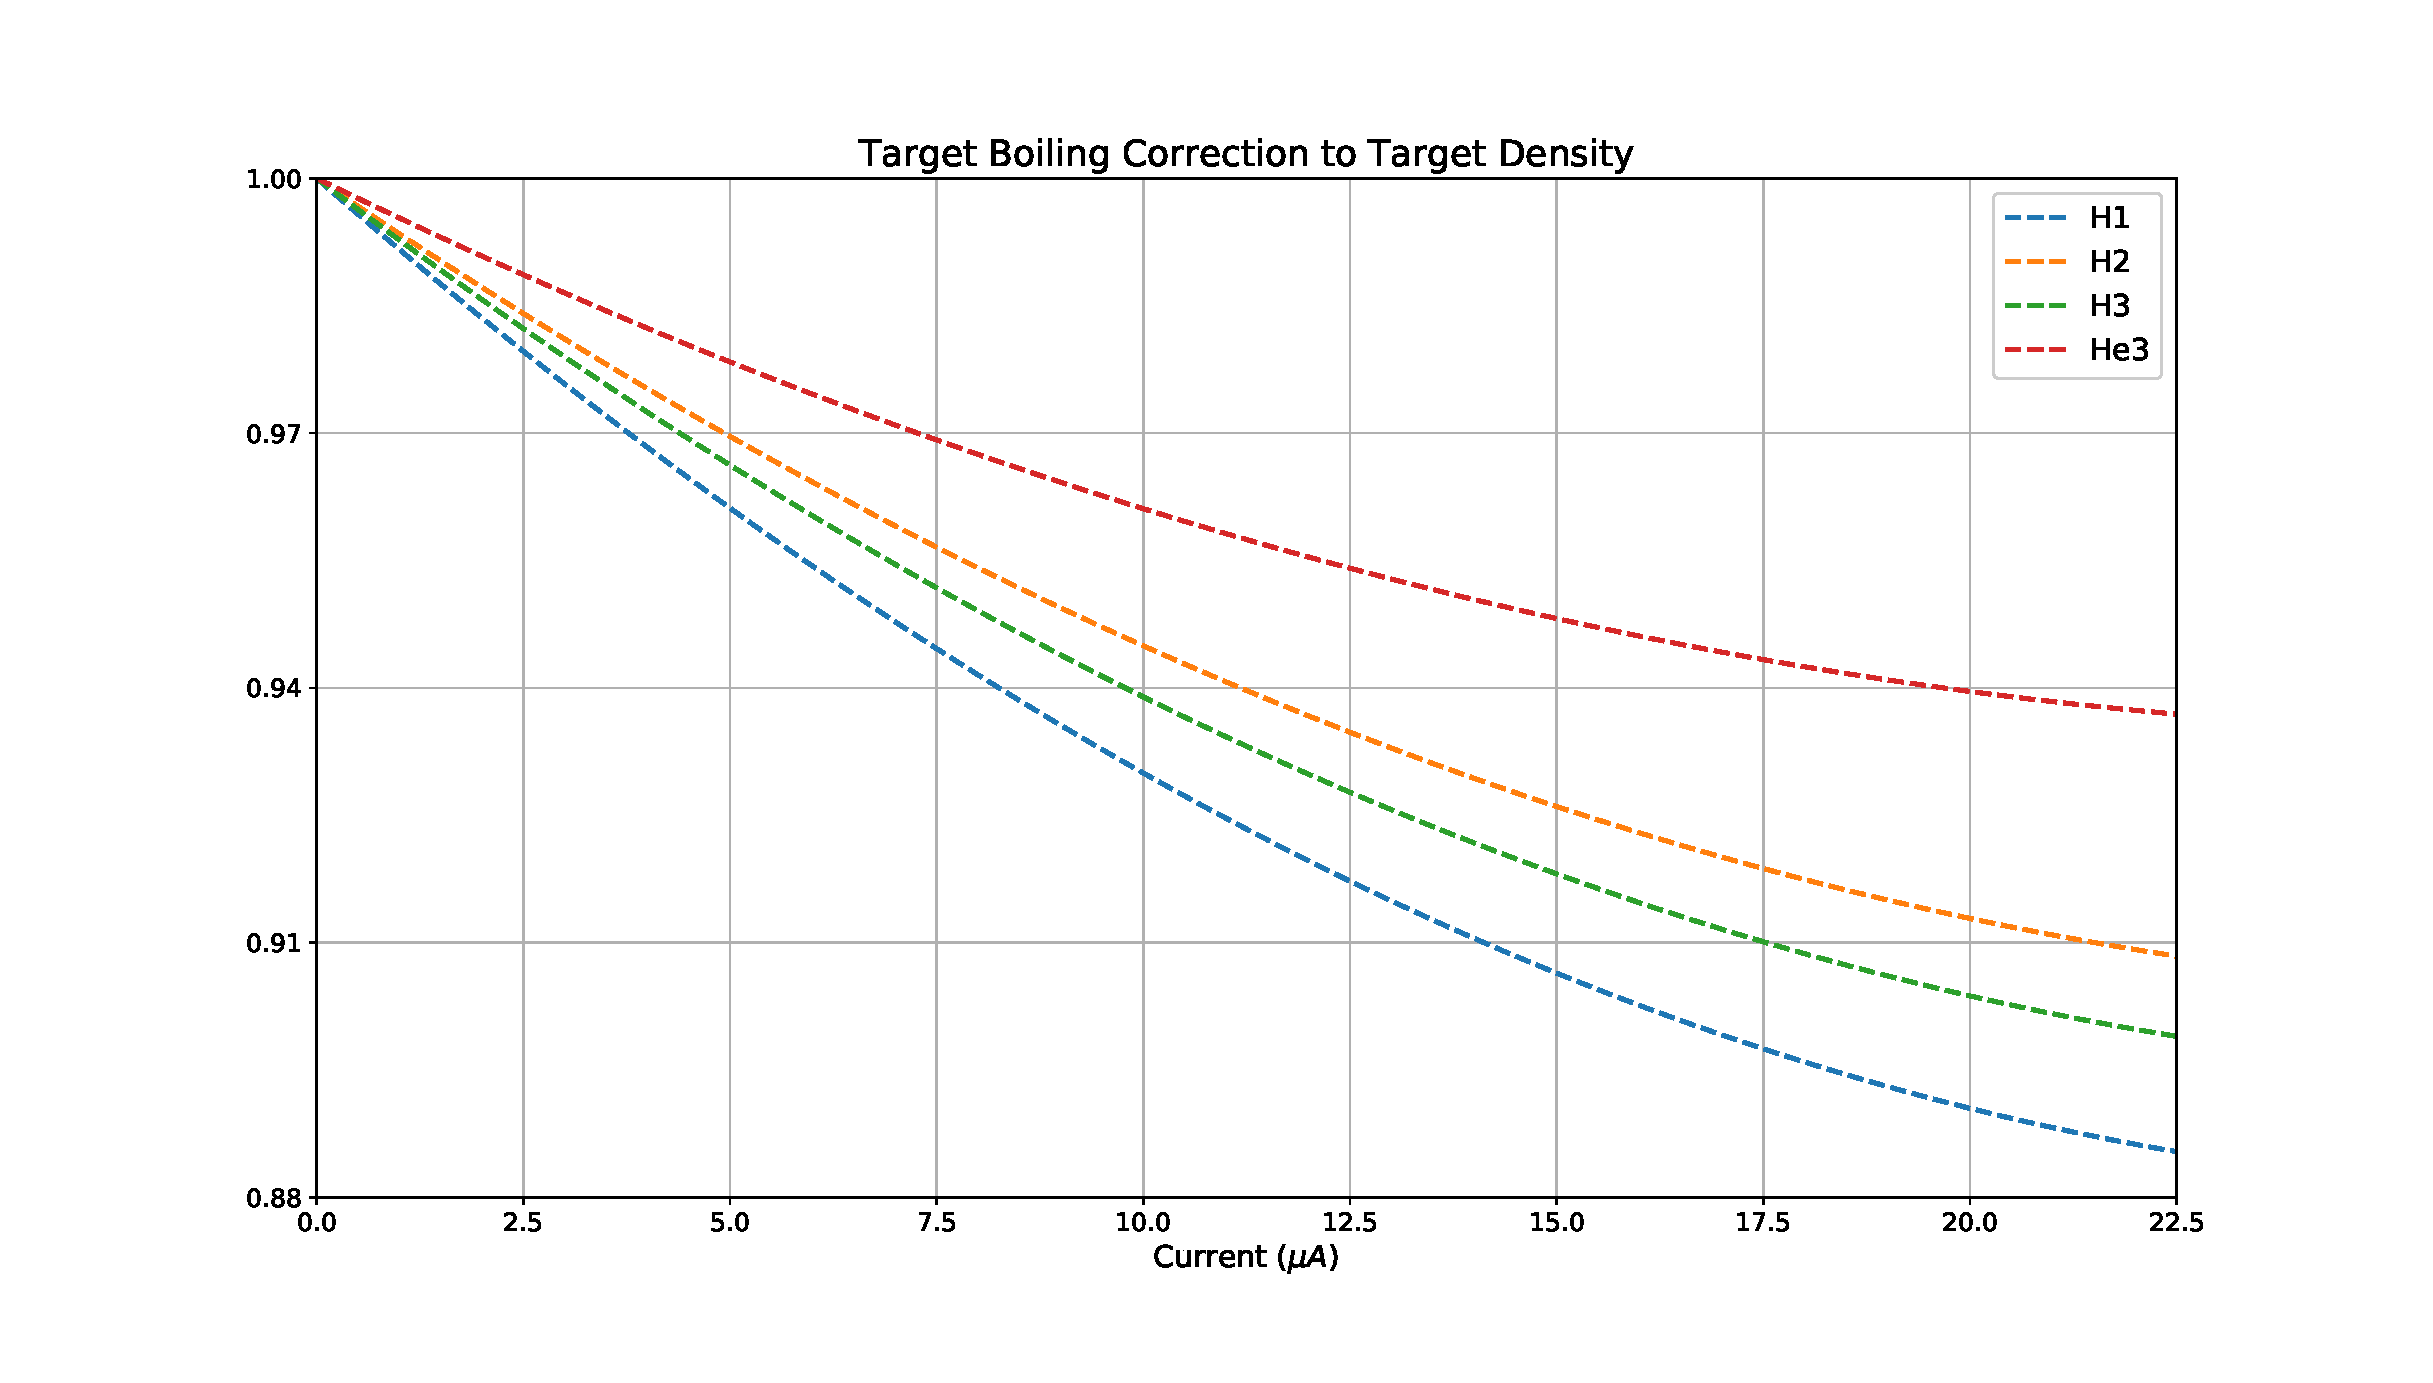
\includegraphics[width=\textwidth]{./analysis/fig/boil_cor.eps}
	\caption{Beam heating effects are manifested as a multiplicative correction to the target density}
	\label{fig:boilcor}
\end{figure}

%\begin{figure}
%	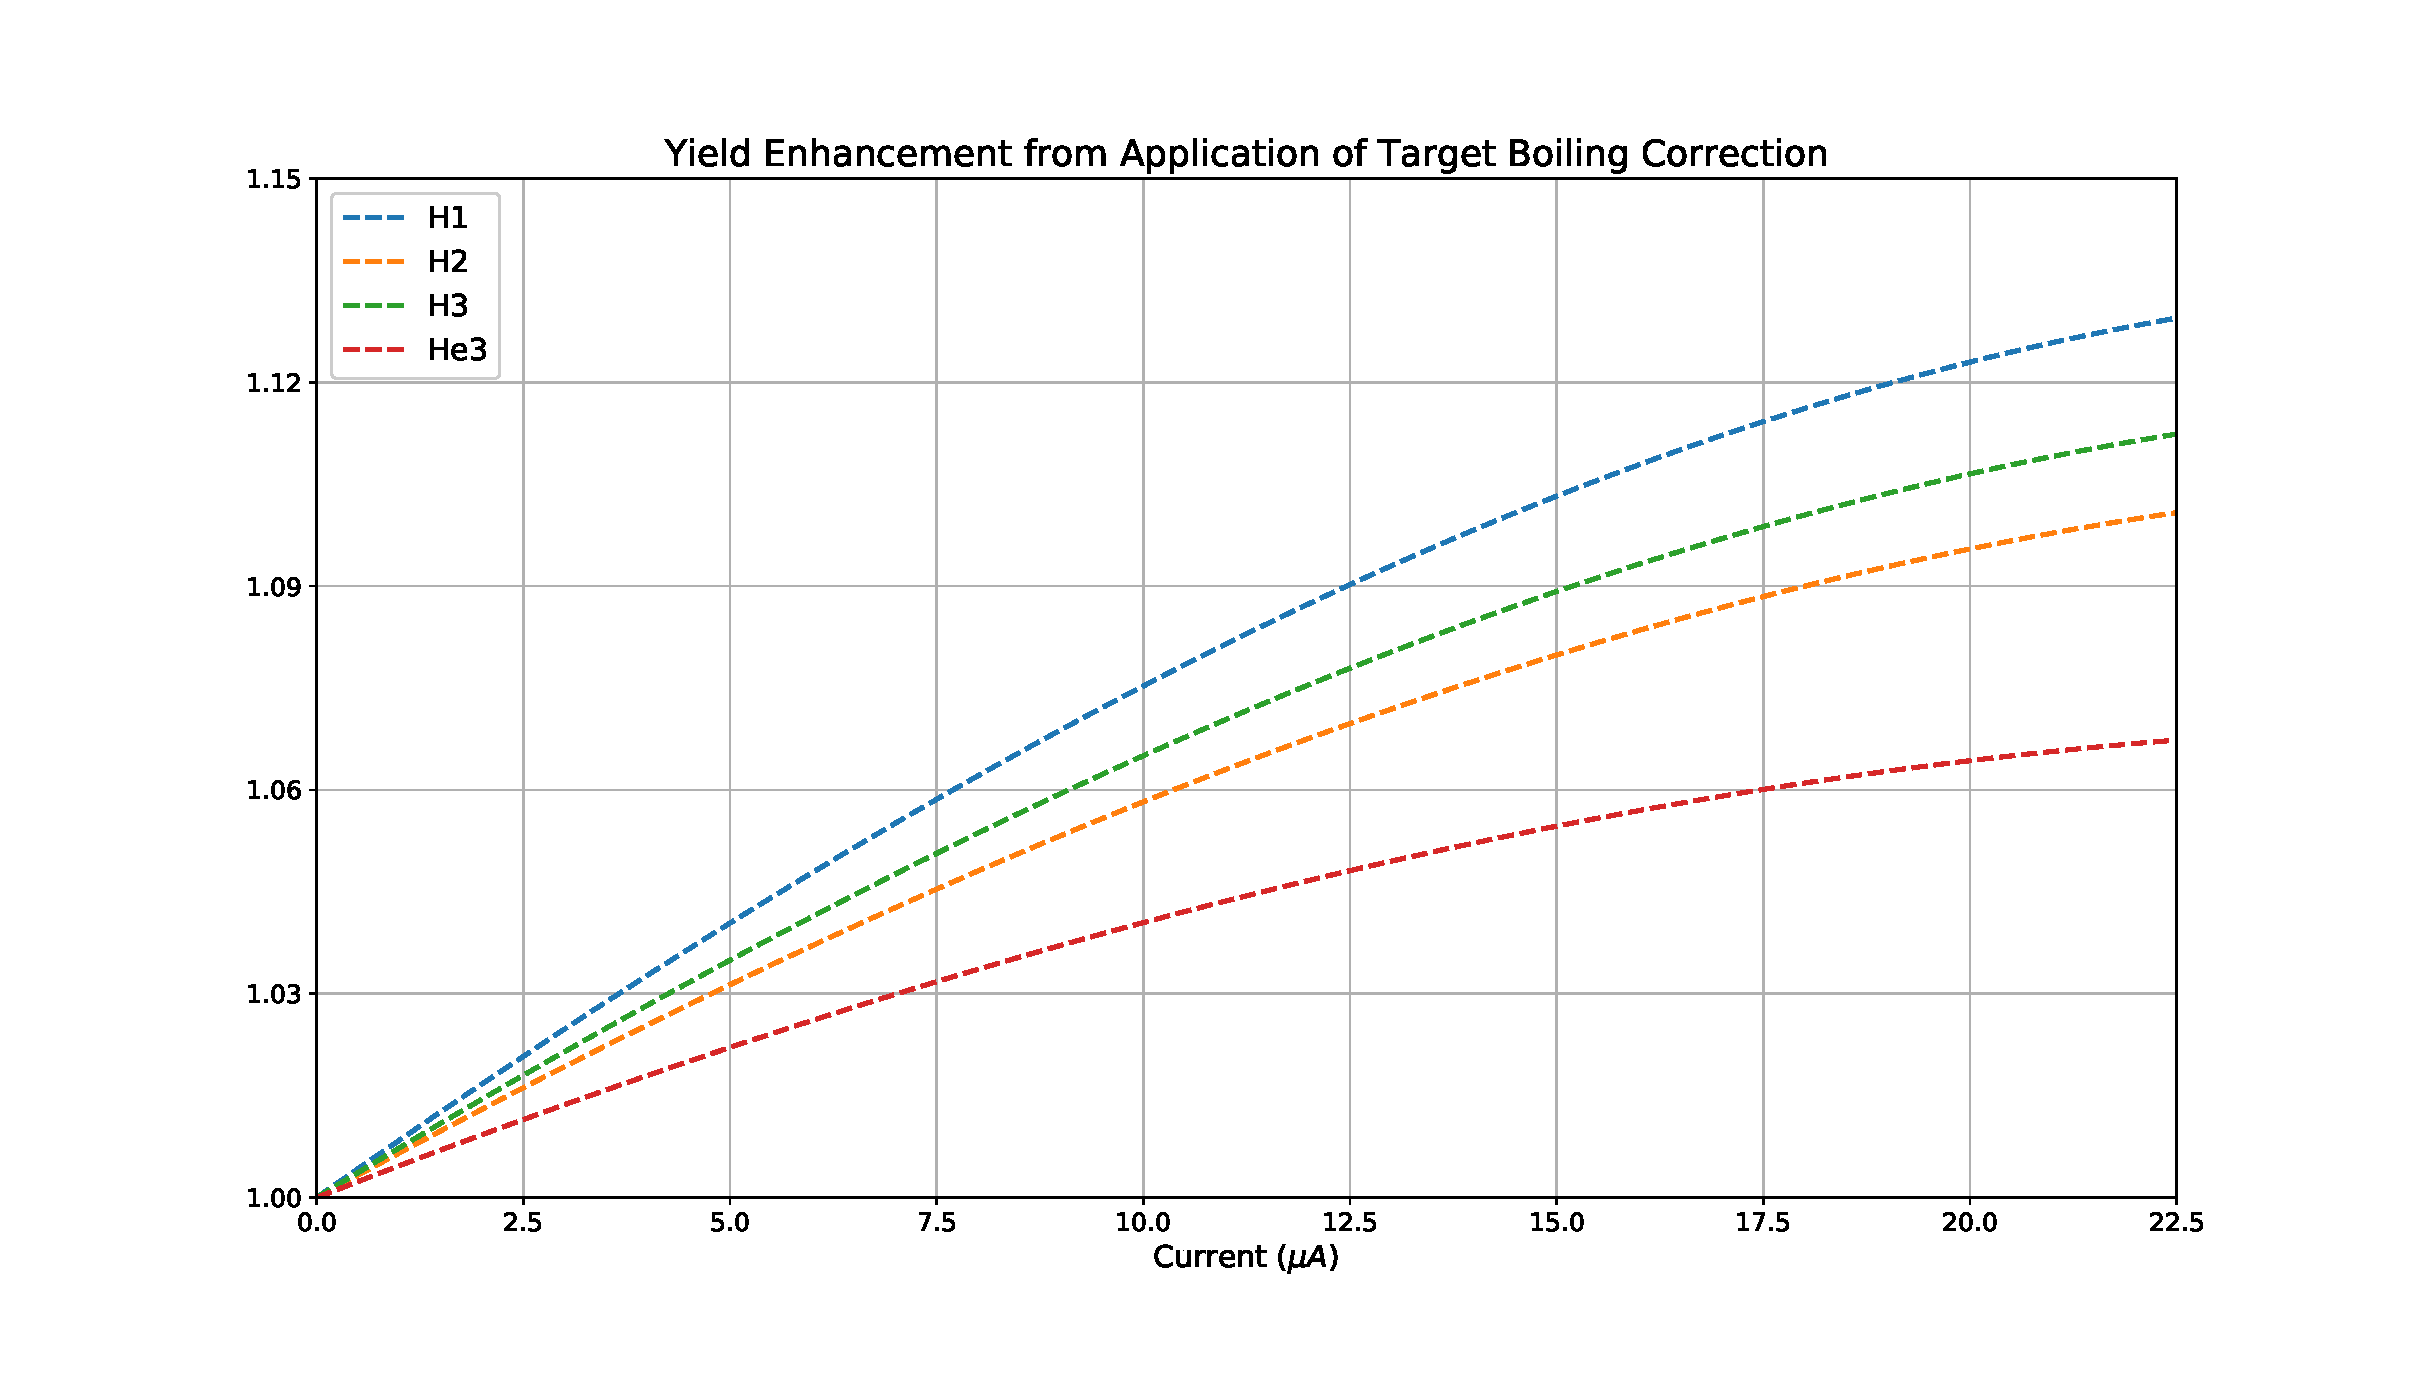
\includegraphics[width=\textwidth]{./analysis/fig/boil_yield_cor.eps}
%	\caption{Target density corrections cause a multiplicative enhancement to the yield}
%	\label{fig:boilyieldcor}
%\end{figure}

\subsection{Target Endcap Contamination}
\label{sec:ecc}

The gas targets used in this experiment are housed in aluminum cells as described in Section \ref{sec:gas_cell}. The thickness of the aluminum greatly exceeds the thickness of the gas and will contribute background that can survive the cuts placed on the data. By quantifying this contribution, the events that originate from the cell endcaps can be subtracted from the final results.

To determine this contribution, the empty cell is used. The empty cell, being an exact replica of the gas target cells with a vacuum inside, allows us to approximately isolate the contribution of the cell walls to the data. The empty cell and the target being studied are compared by calculating the yields on a kinematic-by-kinematic basis and normalizing them by charge and endcap thickness.

The normalization to the endcaps for each target must be done in two parts. This is because each endcap is not the same thickness. When calculating the yield for a target, it is assumed that any contamination upstream (downstream) of the center of the target must originate from the upstream (downstream) endcap. The two halves are then combined to arrive at the endcap thickness normalized yield. This yield calculation only has livetime corrections applied. All cuts are applied except for target length, which is adjusted to only include events upstream (downstream) of the center of the target.

The data for the target being studied and the normalized empty target are then binned in Bjorken $x$. Dividing the empty cell data by the gas target data then gives an approximation of the fractional contribution of the cell walls to the electron data. As this correction is applied to the final results, the contamination corrections for the targets are divided by each other to create the correction to the target ratios. These results are then fit with the functional form $1\pm e^{Ax+B}$. The choice of adding or subtracting the exponential is done by determining if the correction is greater or smaller than 1. The fit function and the covariance matrix of the fit are used to apply the correction to the final results as well as determine the uncertainty contribution of this correction.

\subsection{Charge Symmetric Background Subtraction}

As an inclusive scattering experiment, we are particularly susceptible to background from charge symmetric processes from the target. That is events which involved the production of both an electron and a positron, rather than the electron simply scattering. To study this, the polarity of the LHRS was reversed so that positively charge particles are directed into the detectors rather than negatively charged particles. With this setting, a number of runs were taken in kinematics 0 through 5. These runs were taken with all targets, just as the electron data was taken. This allows for a measurement of the positron yield which corresponds to a measure of the charge symmetric background.

This measurement allows us to determine the proportion of electrons that originated from pair production. Applying the same cuts and as the electron data allows us to determine the charge normalized positron yield. Unlike in the electron analysis, it was noted that there was significant pion contamination in the positron data. This pion contamination had to be subtracted in order to get an accurate calculation of the positron yield. This is achieved by fitting the main pion peak and the subtracting the tail of the fit which survives the cuts applied from the positron data.

The charge normalized positron yields over these kinematics are then combined (using the same methods as the electron yield) and binned in Bjorken $x$. This was then divided by the charge normalized electron yield. This is a fractional measure of the charge normalized background contamination. The ratio is then fit with an exponential of the form $e^{Ax + B}$, where $A$ and $B$ are the fit parameters. These fits are shown in in Figure \ref{fig:positrons}.

This correction is applied to the final yield ratio results. Both the numerator and denominator must have the charge symmetric background subtracted. Each target yield in the ratio is scaled by $1 - \left(\textrm{Charge Symmetric Background Fit}\right)$. For each bin, the fit is calculated at the bin center.

\begin{figure}
	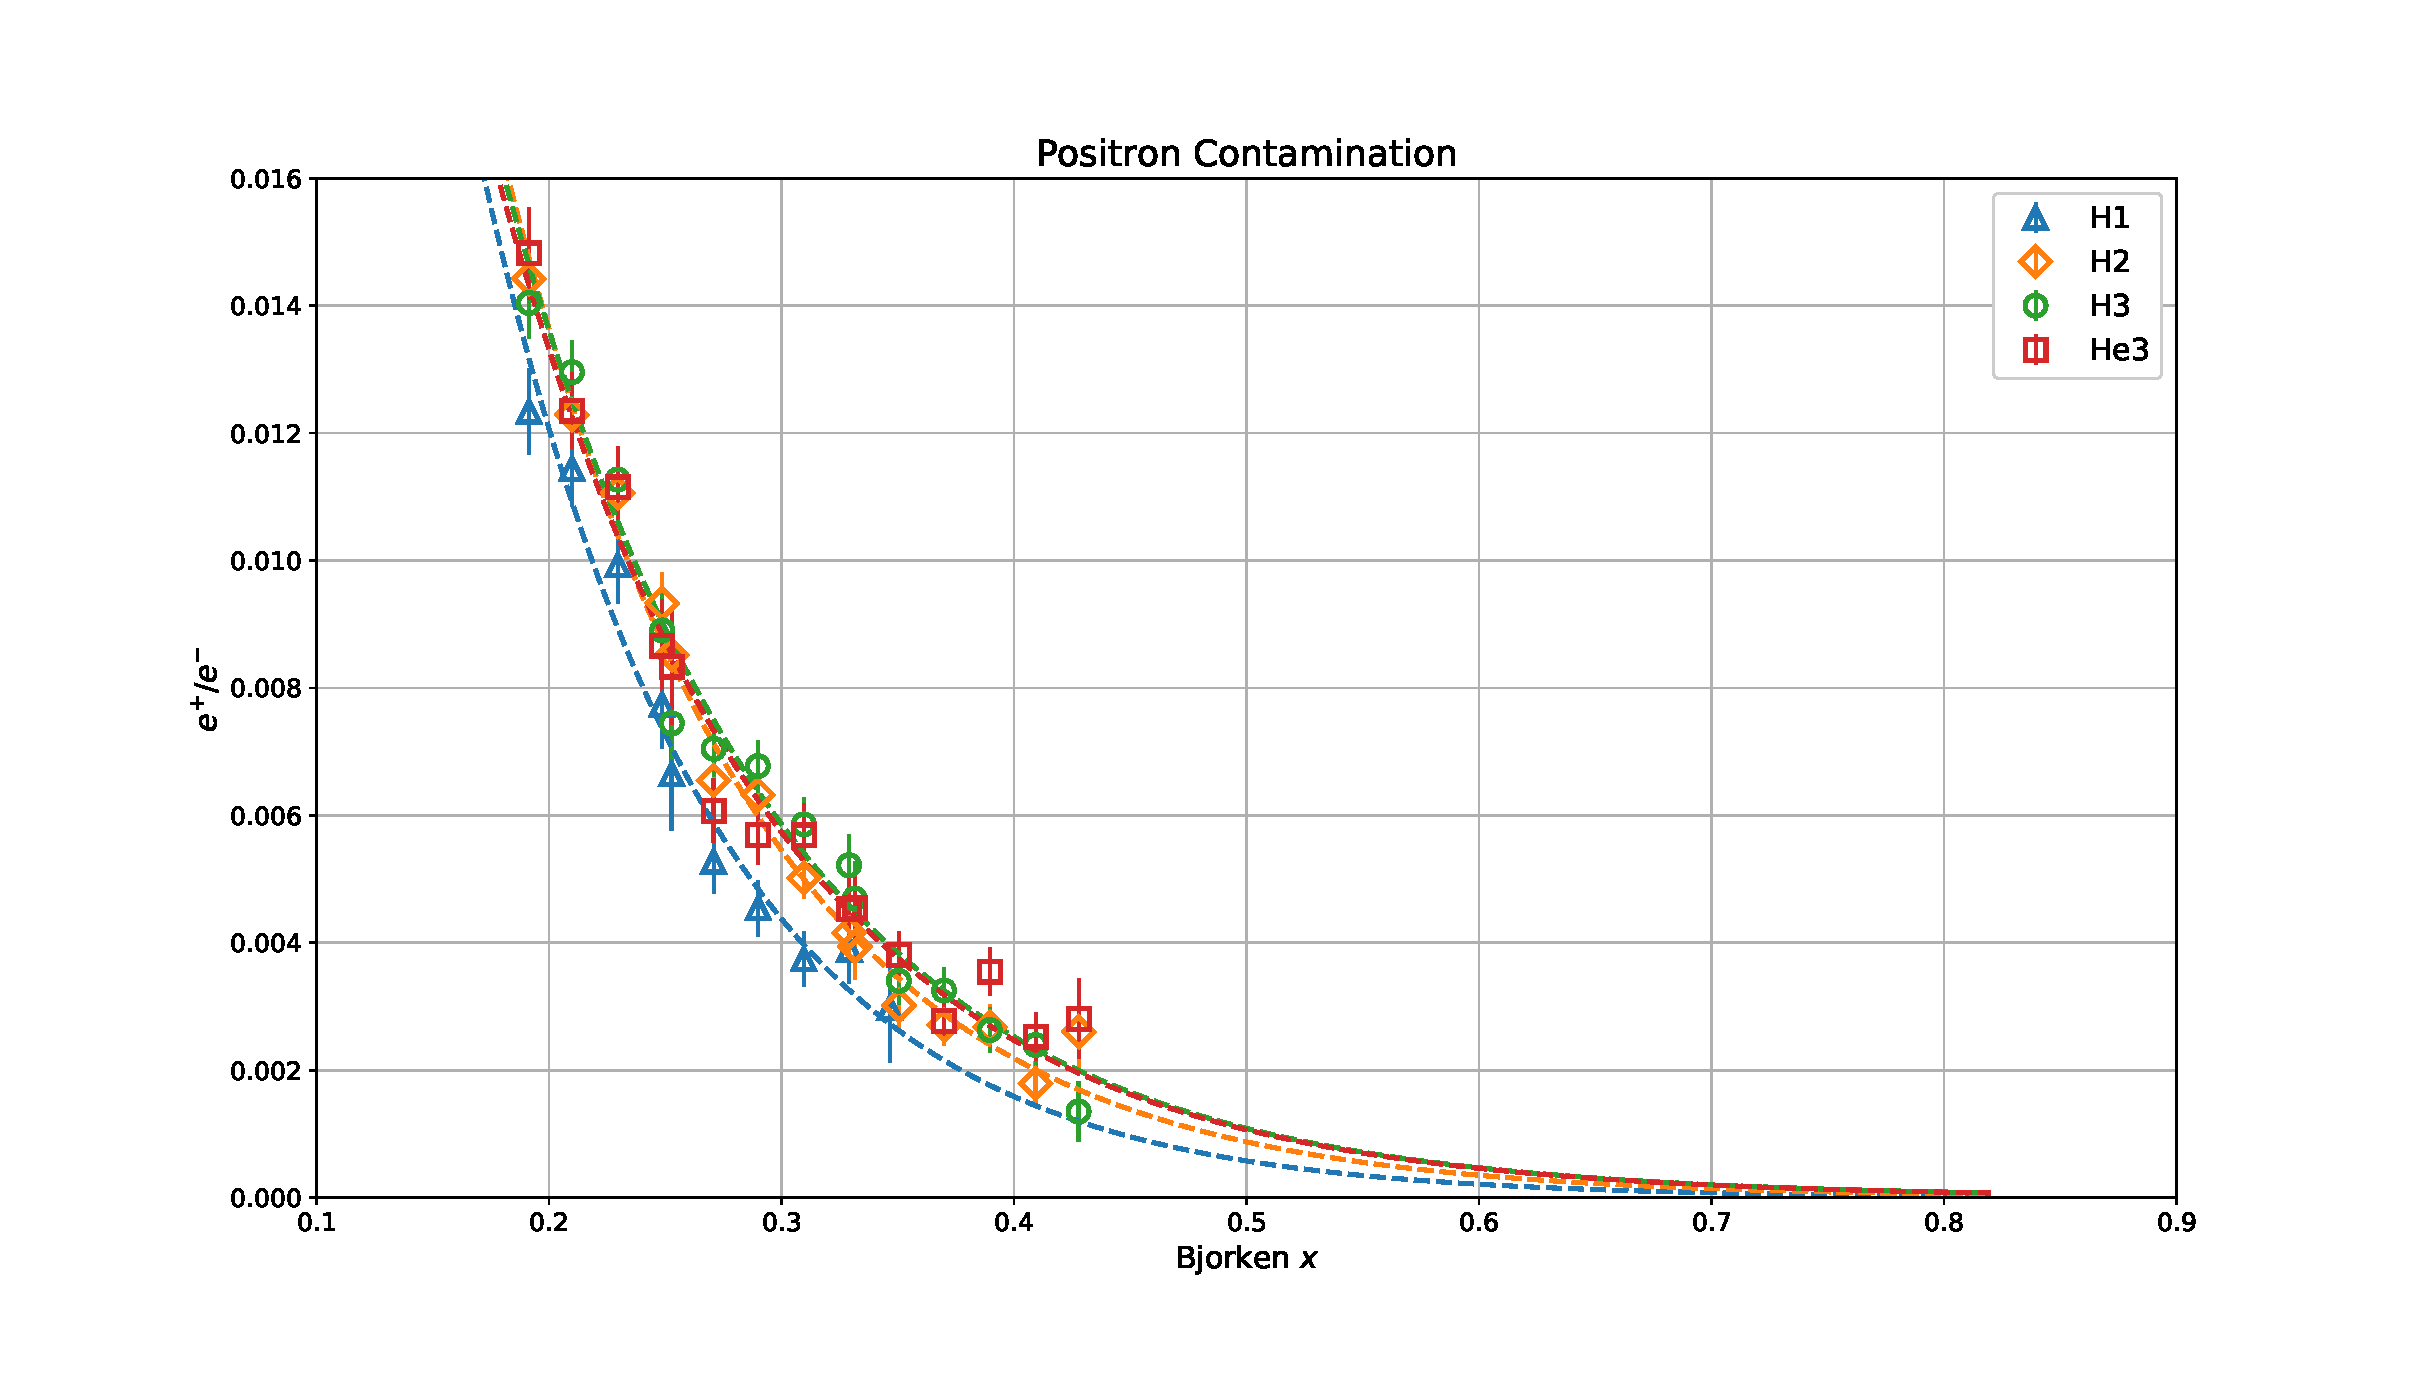
\includegraphics[width=\textwidth]{./analysis/fig/positrons.eps}
	\caption{Charge symmetric background correction}
	\label{fig:positrons}
\end{figure}

\subsection{Computer Deadtime Correction}

Our DAQ unable to continuously record data. While we can probabilistically determine the mean time spacing between events, in the real world events can deviate greatly from these means. Sometimes events will occur that are too close in time for our DAQ to record as the computer has not completed recording the previous event. Deadtime is a function of event rate; when events happen more rapidly, there is a higher chance that events will occur too closely in time to be recorded.

When deadtime is low and the number of recorded events is high, it is a reasonable assumption that the events recorded will accurately reflect the distribution of events in the ``zero-deadtime limit''. In this case correcting for the deadtime is simply done by scaling the number of events by the ``livetime'' of the experiment.

The computer livetime was measured using the Trigger Supervisor and scalers in each HRS. The trigger signals generated from detector signals are copied and sent to both the Trigger Supervisor and a scaler unit. The Trigger Supervisor is subject to the computer deadtime event loss discussed here. The scaler unit, on the other hand, simply increments a register when a trigger signal is received. The ratio of these the number of events recorded by these two systems gives a measure of the livetime of the measurement. The livetime is defined on a run-by-run basis as:

\begin{equation}
DT = \frac{\Sigma \mathrm{Triggers_{TS}}}{\Sigma \mathrm{Triggers_{Scaler}}}
\end{equation}

In an ideal world, the deadtime will be identical for all runs within a kinematic. However, the deadtime is measured on a run-by-run basis and is applied as such in order to account for any deviations from this assumption. The average deadtime for each target in each kinematic is plotted in Figure \ref{fig:deadtime}.

\begin{figure}
	\includegraphics[width=\textwidth]{./analysis/fig/deadtime.eps}
	\caption{Deadtime per kinematic}
	\label{fig:deadtime}
\end{figure}

\subsection{Radiative Corrections}

The Deep Inelastic Cross Sections being studied are the Born approximation of a single-photon exchange. The measurement however, contains contributions from higher order processes that will increase the measured cross section. Using a model, the contributions can be corrected for and removed from the measurement.

The experiment used a software package called $\texttt{T2\_EXTERNALS}$ that calculates both the Born cross section and the radiated cross section for a given target at a kinematic set $(E,E^{\prime} ,\theta )$.

\subsection{Isoscalar Corrections}

\subsection{Bin Centering Corrections}

The cross-section over the width of a bin is not constant. This means that the measurement does not correspond with the true cross section at the center of the bin. Using a model that matches the shape of our data well, the location of the measurement within the bin can be calculated. This is done by calculating the expectation value of the model within that bin and determining the $x$ value corresponding to this value. The expectation value is given by
\begin{equation}
	\langle f_{\rm measured}\rangle = \frac{1}{\Delta x}\int_{x_{\rm low}}^{x_{\rm high}} f\left( x \right) dx,
\end{equation}
where $f$ is a function representing the chosen model. In practice, the $x$ value does not need to be calculated if the data will be reported at the bin center. Rather, the correction is simply the ratio of the model at the bin center. This is written as
\begin{equation}
	\sigma_{\textrm{Bin Centered}} = \frac{f\left(x_{\textrm{Bin Center}}\right)}{\langle f_{\rm measured}\rangle} \sigma_{\rm measured}.
\end{equation}

This correction must be applied to both targets in the ratios. That is, the ratio must be multiplied by the correction to the numerator and divided by the correction to the denominator.\cite{wtsydp}

\subsection{Coulomb Corrections}

Corrections must be made for the effect of the charge of the target on the scattered electron. This interaction causes the $Q^2$ of the event to shift to an effective $Q^2$ value, $Q^2_{\rm eff}$. This conversion is done with the equation
\begin{equation}
	Q^2_{\rm eff} = Q^2 \left(1 + \frac{3Z\alpha\hbar c}{2RE}\right)^{2}.
\end{equation}
In this equation $R$ is the hard-sphere equivalent radius of the nucleus which is defined as $R=\left[\left(\nicefrac{5}{3}\right) \langle r^{2}\rangle\right]^{\nicefrac{1}{2}}$ where $\langle r^2\rangle$ is the root-mean-squared radius of the nucleus.\cite{coulomb}

Using $x=\frac{Q^2}{2M\nu}$, it is clear that a shift in $Q^2$ will result in a proportional shift in $x$. Using a model cross-section, the cross section is calculated at both the nominal $x$ and at $x_{\rm eff}$. As the results have been bin centered, this calculation uses a nominal $x$ at the center of the bin. This will lead to the correction
\begin{equation}
	\sigma_{\textrm{Coulomb Corrected}} = \sigma_{\rm data} \frac{\sigma_{\rm model}\left(x_{\rm eff}\right)}{\sigma_{\rm model}\left(x\right)}.
\end{equation}

This correction must be applied to both targets in the ratios that are calculated.
\subsection{Particle Identification}


\chapter{\bf{The EMC Effect}}             % Chapter  1
\setcounter{figure}{0}
\setcounter{table}{0}
\setcounter{equation}{0}
\section{Yield Calculation}

The MARATHON experiment measured cross section ratios. This method allows us to cancel many systematics that would otherwise plague a full cross section analysis. By taking data for each target at the same kinematics, acceptance effects are identical. This data taking technique means that with reasonable acceptance cuts, a ratio of target yields is wholly equivalent to the ratio of cross sections.

To calculate the yield we use a simple equation:

\begin{equation}
	\text{Yield} = \frac{\text{Counts}}{\text{Scattering Centers} \cdot \text{Livetime}} \cdot \text{Corrections}
\end{equation}

The yield is binned in Bjorken $x$. This chapter will explain the cuts and corrections that go into this calculation.

\section{Calibration}
\subsection{Raster Calibration}
The raster is calibrated by defining a line that maps the raster current to positions at each BPM and the target. To do this, the slope and intercept of this line had to be determined. The slope corresponds to the conversion of raster current to position displacement. The intercept is then determined from the central position that the beam is displaced from. This section will be a general presentation of the techniques used to calibrate the raster. For a more in-depth discussion of how the raster was calibrated, see Appendix \ref{raster_appendix}.

For the horizontal raster, this was done by optimizing the reconstructed z-vertex on the target. When properly calibrated, there should be no correlation between the horizontal raster and the z-vertex. Linear interpolation between two ``bad'' calibrations is a simple way to determine the correct calibration slope.

The veritcal raster could be calibrated in a similar way by minimizing the correlation between the vertical raster and a known momentum phenomena (i.e. a $W^2$ peak). Unfortunately, such a feature does not exist within the kinematics of MARATHON data. The vertical calibration was determined using the carbon hole target. The hole is known to be $2mm$ diameter. By using the raster data, the hole can be fit in order to determine the vertical calibration slope.

The intercepts are determined by looking at the mean BPM position readings and projecting these to the target. This position will correspond to the mean value of the rasters as well. Using the beam position, raster current, and calibration slope the calibration intercept can easily be determined.


\section{Analysis}
\section{Corrections}

When analyzing the data, there are several corrections that need to be made. These are due to various physical or systematic effects that took place during the experiment. These effects have been studied in order to determine a ``correction factor'' that can be applied to the data.

\subsection{Target Boiling}
\label{sec:boiling}

When the beam is incident on the target, it deposits heat into the gas. This causes a density fluctuation of the gas referred to as ``target boiling''. The target does not actually boil, however that is the standard nomenclature for a density fluctuation in a gas target. When the density of the target changes, it changes the effective target thickness as seen by the beam. When the target thickness changes, there is a changed number of scattering centers which will lead to a change in the number of electrons recorded. Specifically, heating will decrease the target density which will decrease the number of scattered electrons.

The density changes are a function of the current on the target. Each run is taken at a single current so that the correction can be applied run by run. The correction is approximately linear for small deviations in current. A study of the effect during beam ramping found that the density settles very quickly. This means that so long as we cut events that occur with the beam off, it is unnecessary to take into account the beam ramping when correcting for this effect.

To determine the correction, a dedicated set of runs was taken with the Left HRS spectrometer at $16.8\degree$ and 3.1 GeV. At this kinematic, several data runs were recorded with varying current between them. Each of these runs were analyzed with the standard data cuts to determine the yield. This allows for the yield to be determined as a function of beam current.

Now that the yields have been determined as a function of beam current, they can be plotted and fit. The data is fit with a quadratic polynomial. This fit is constrained to require no correction (a correction factor of 1) at zero current. This is because the density must be the nominal fill density when there is no beam heating. During analysis the average current is calculated for a run (ignoring beam trips). The average current is then used to calculate the target density correction with the fit function. The correction is then applied on a run-by-run basis by multiplying the number of scattering centers by this correction factor (or equivalently dividing the yield by the correction factor). Figure \ref{fig:boilcor} shows the correction factors for each target.\cite{boiling}

\begin{figure}
	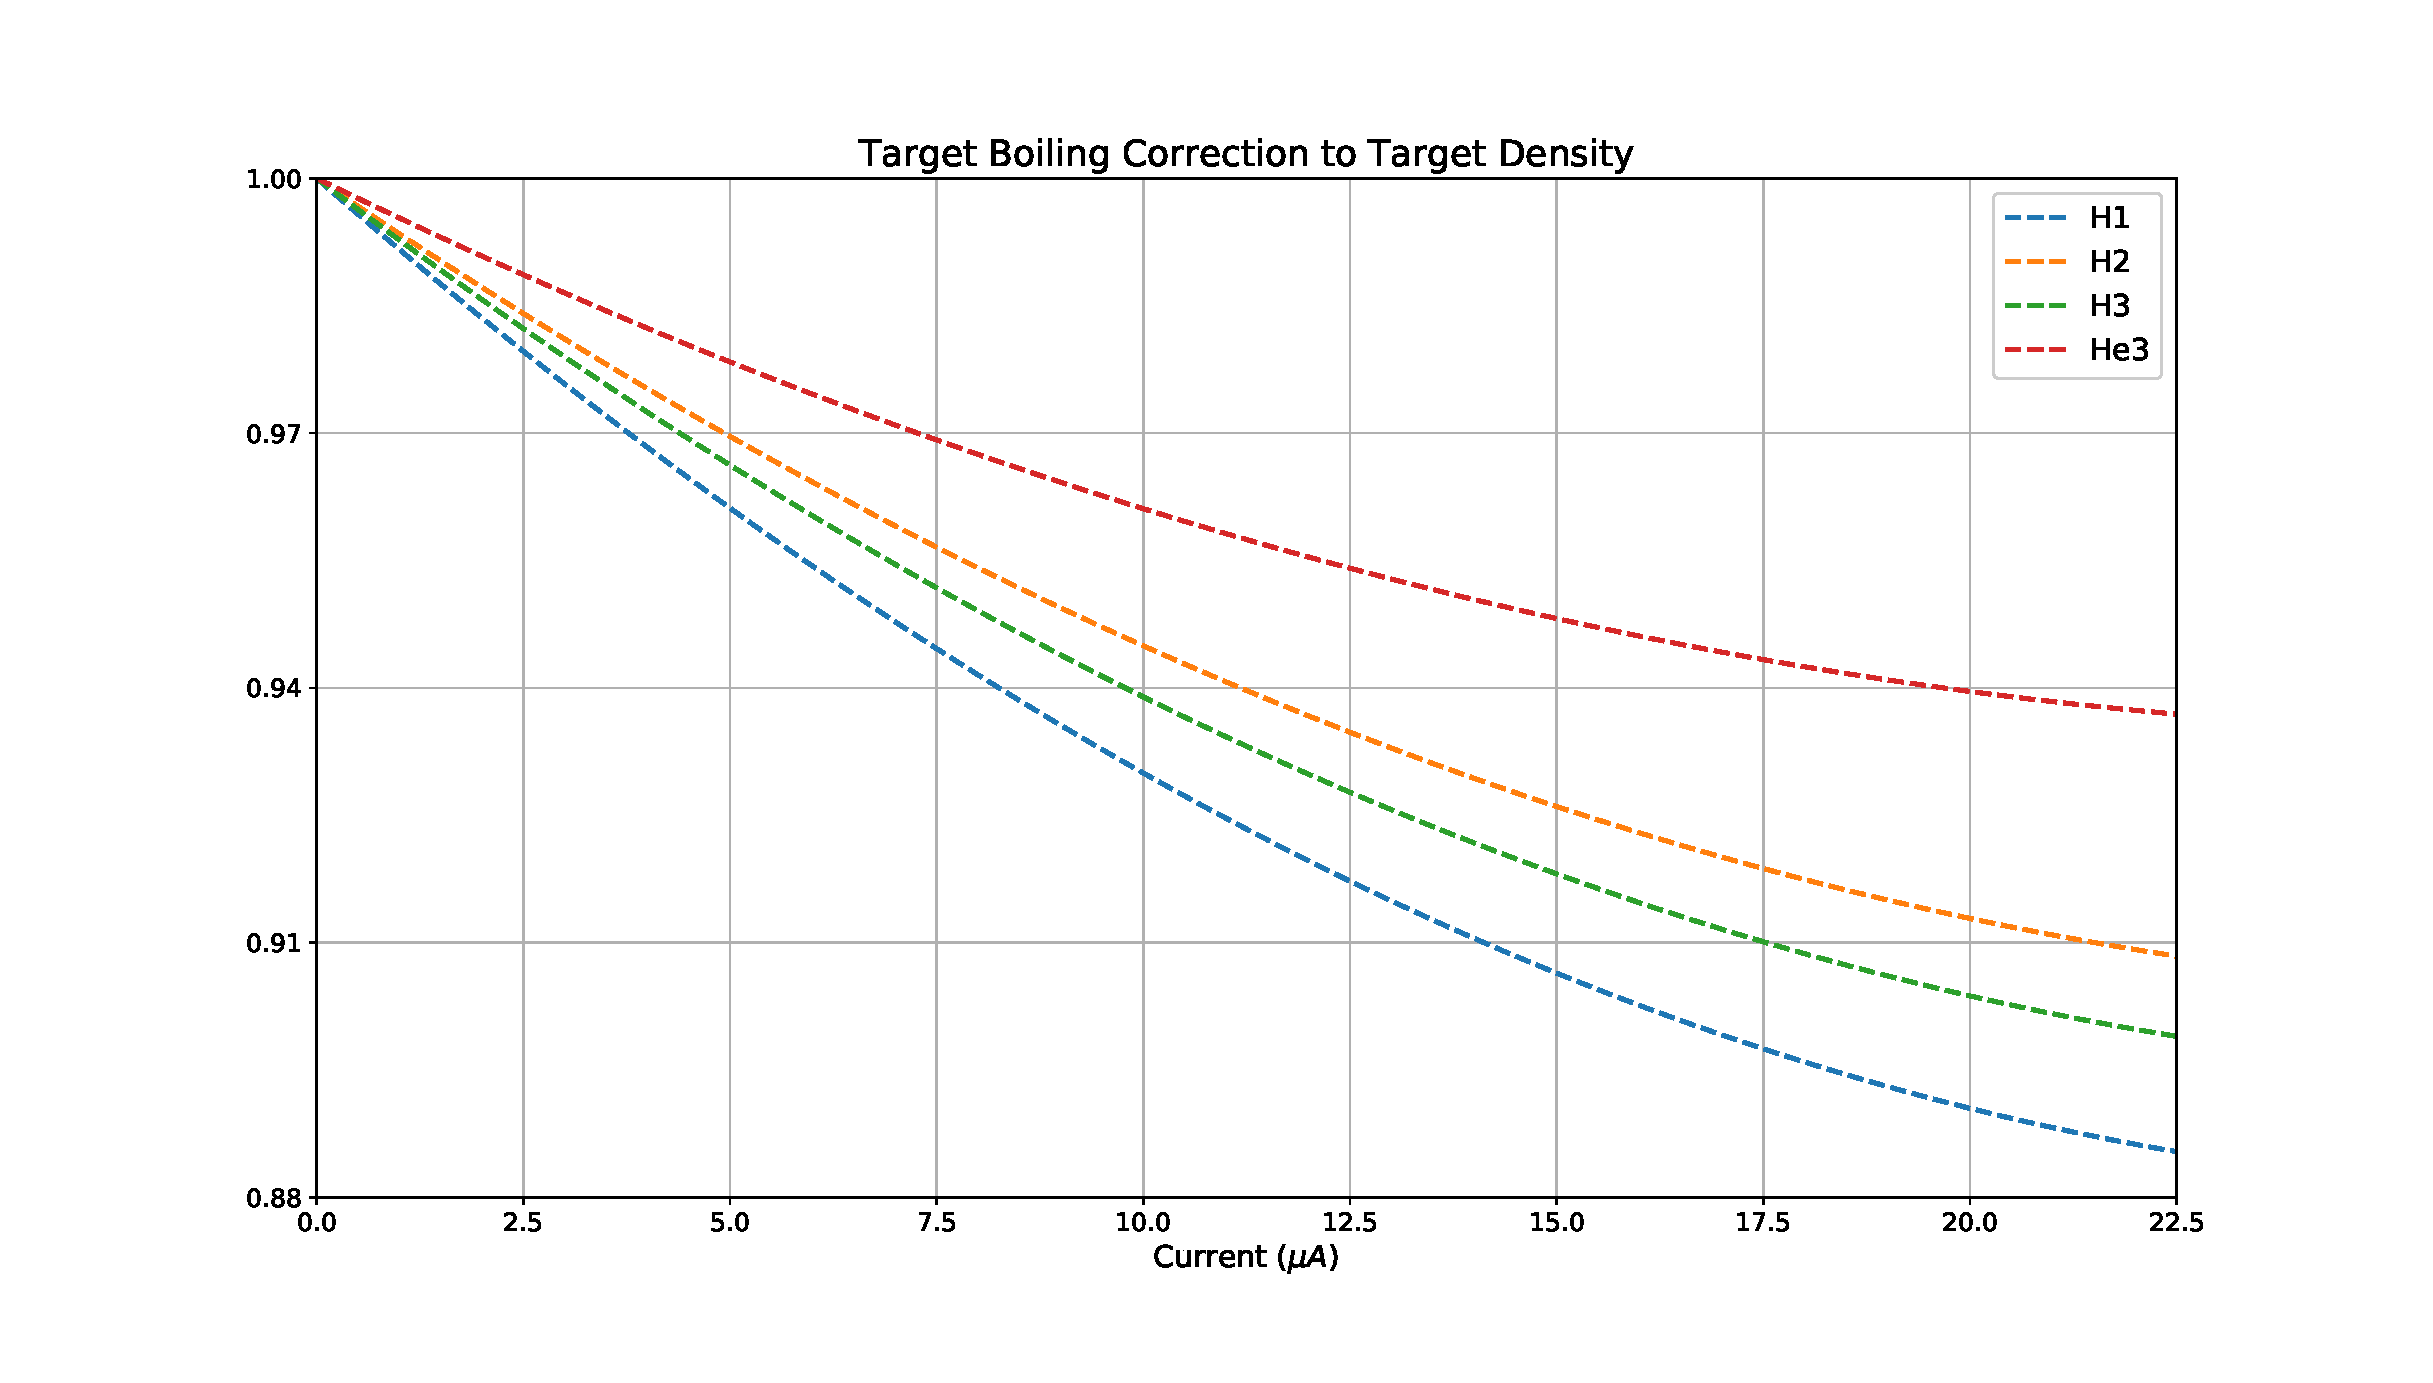
\includegraphics[width=\textwidth]{./analysis/fig/boil_cor.eps}
	\caption{Beam heating effects are manifested as a multiplicative correction to the target density}
	\label{fig:boilcor}
\end{figure}

%\begin{figure}
%	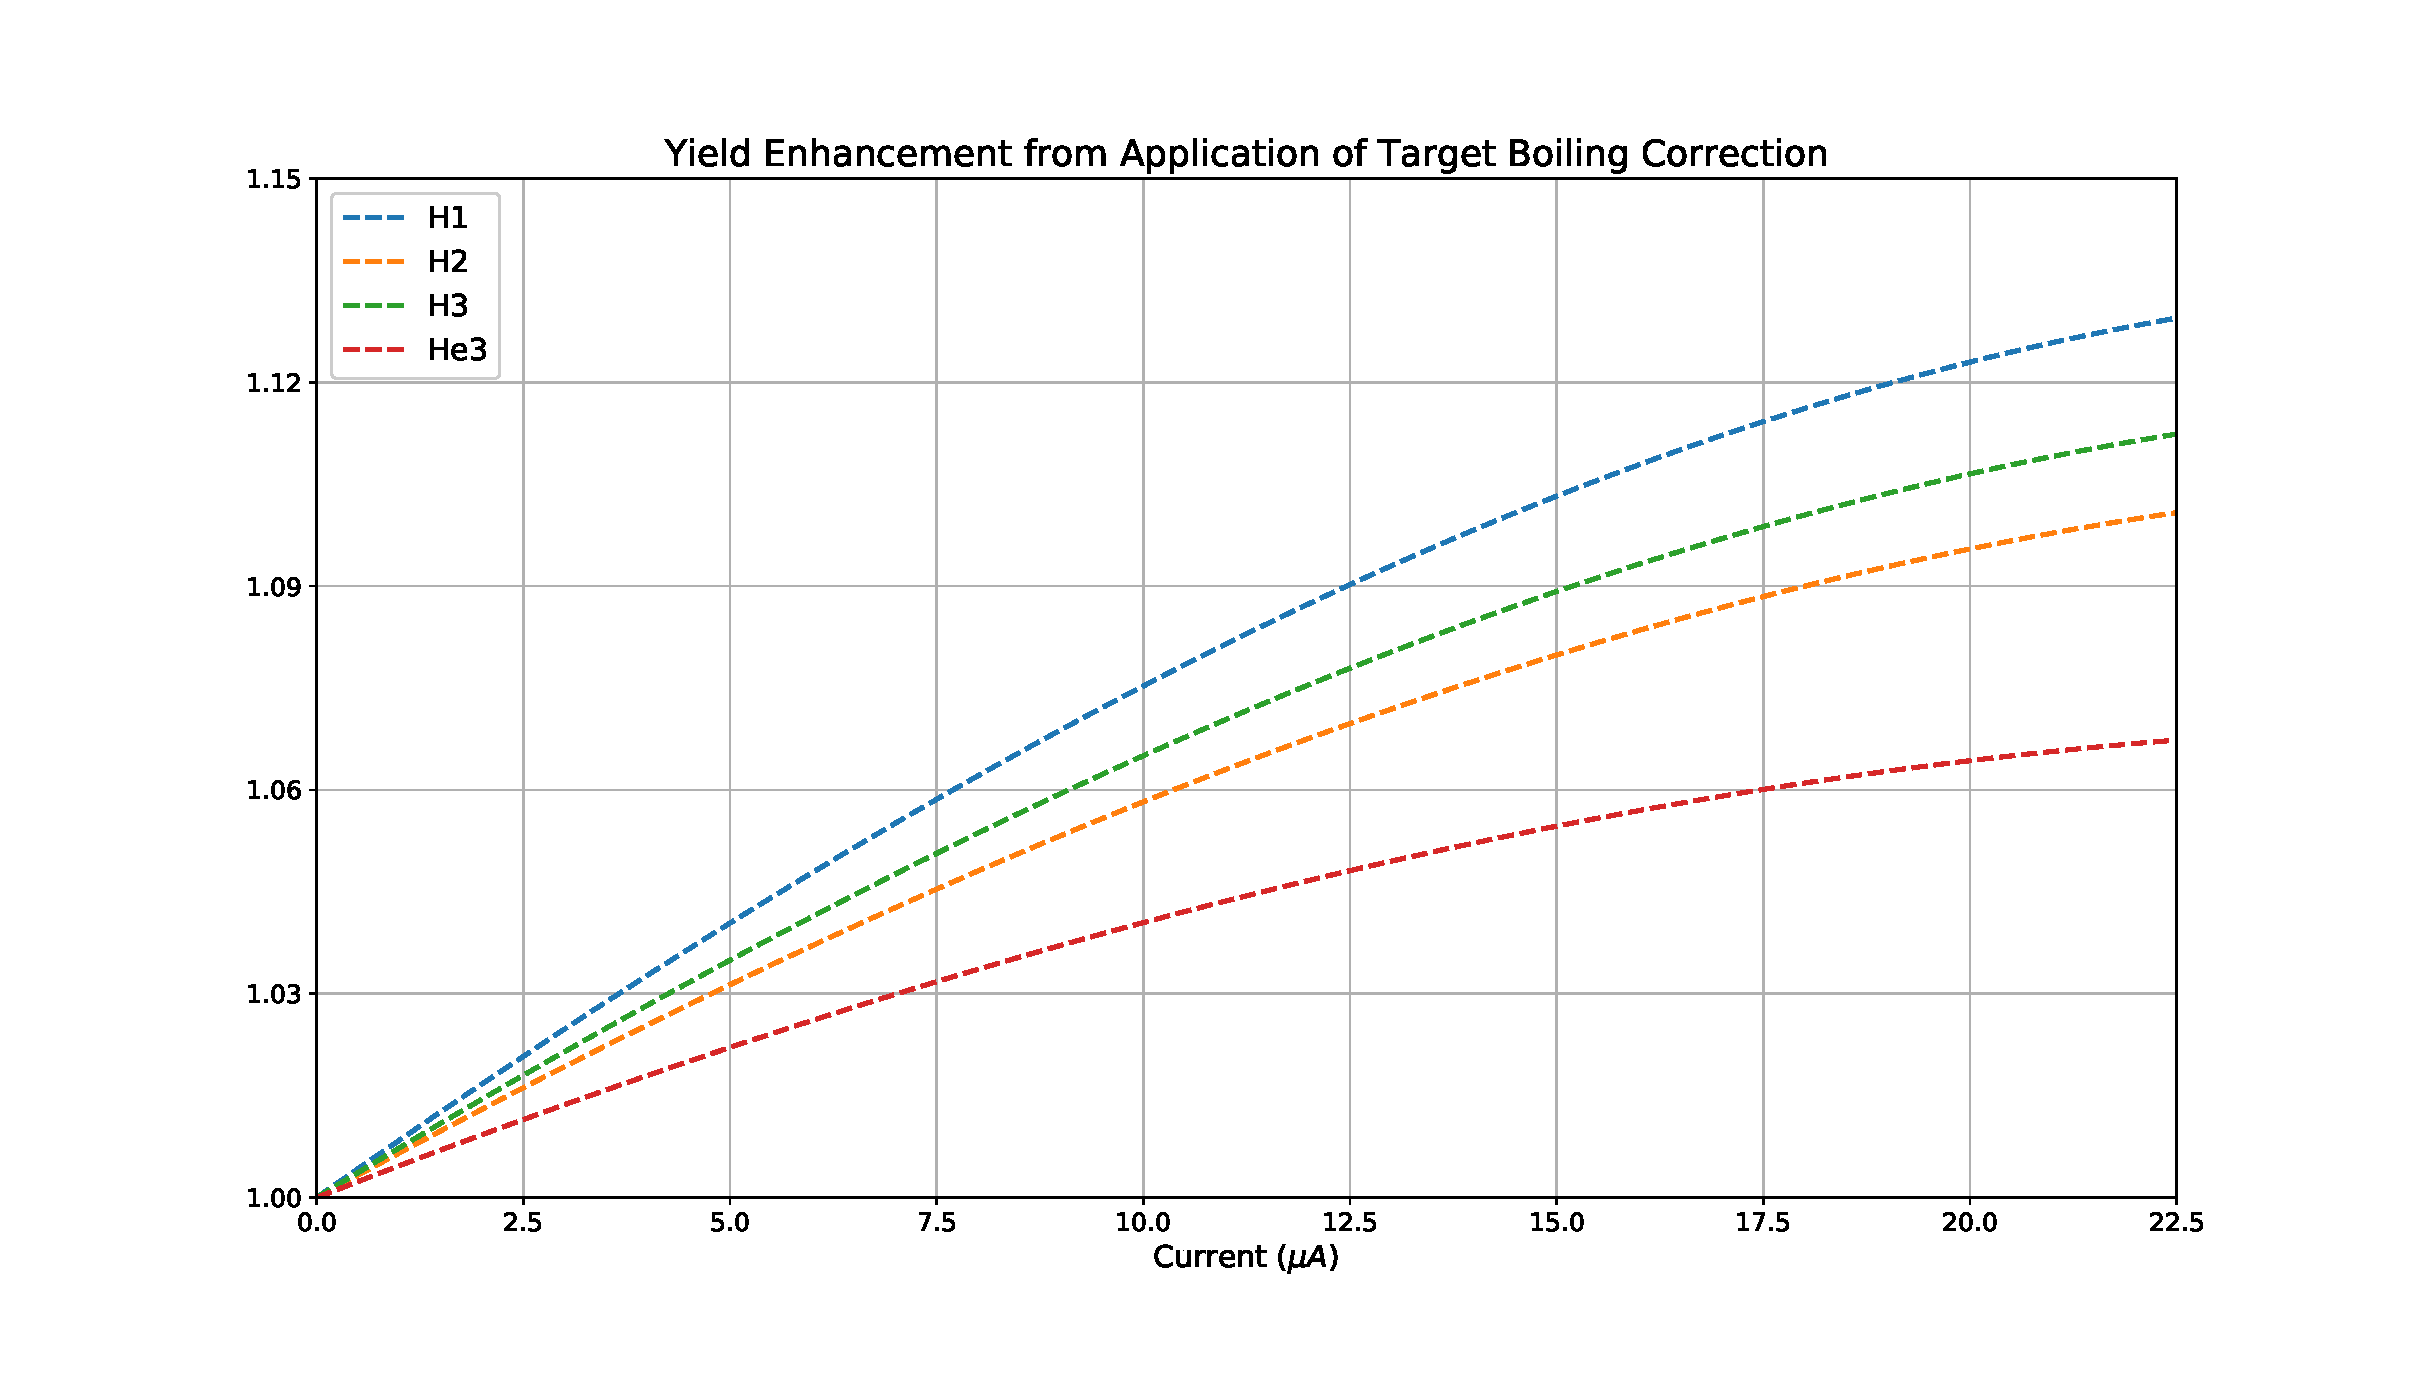
\includegraphics[width=\textwidth]{./analysis/fig/boil_yield_cor.eps}
%	\caption{Target density corrections cause a multiplicative enhancement to the yield}
%	\label{fig:boilyieldcor}
%\end{figure}

\subsection{Target Endcap Contamination}
\label{sec:ecc}

The gas targets used in this experiment are housed in aluminum cells as described in Section \ref{sec:gas_cell}. The thickness of the aluminum greatly exceeds the thickness of the gas and will contribute background that can survive the cuts placed on the data. By quantifying this contribution, the events that originate from the cell endcaps can be subtracted from the final results.

To determine this contribution, the empty cell is used. The empty cell, being an exact replica of the gas target cells with a vacuum inside, allows us to approximately isolate the contribution of the cell walls to the data. The empty cell and the target being studied are compared by calculating the yields on a kinematic-by-kinematic basis and normalizing them by charge and endcap thickness.

The normalization to the endcaps for each target must be done in two parts. This is because each endcap is not the same thickness. When calculating the yield for a target, it is assumed that any contamination upstream (downstream) of the center of the target must originate from the upstream (downstream) endcap. The two halves are then combined to arrive at the endcap thickness normalized yield. This yield calculation only has livetime corrections applied. All cuts are applied except for target length, which is adjusted to only include events upstream (downstream) of the center of the target.

The data for the target being studied and the normalized empty target are then binned in Bjorken $x$. Dividing the empty cell data by the gas target data then gives an approximation of the fractional contribution of the cell walls to the electron data. As this correction is applied to the final results, the contamination corrections for the targets are divided by each other to create the correction to the target ratios. These results are then fit with the functional form $1\pm e^{Ax+B}$. The choice of adding or subtracting the exponential is done by determining if the correction is greater or smaller than 1. The fit function and the covariance matrix of the fit are used to apply the correction to the final results as well as determine the uncertainty contribution of this correction.

\subsection{Charge Symmetric Background Subtraction}

As an inclusive scattering experiment, we are particularly susceptible to background from charge symmetric processes from the target. That is events which involved the production of both an electron and a positron, rather than the electron simply scattering. To study this, the polarity of the LHRS was reversed so that positively charge particles are directed into the detectors rather than negatively charged particles. With this setting, a number of runs were taken in kinematics 0 through 5. These runs were taken with all targets, just as the electron data was taken. This allows for a measurement of the positron yield which corresponds to a measure of the charge symmetric background.

This measurement allows us to determine the proportion of electrons that originated from pair production. Applying the same cuts and as the electron data allows us to determine the charge normalized positron yield. Unlike in the electron analysis, it was noted that there was significant pion contamination in the positron data. This pion contamination had to be subtracted in order to get an accurate calculation of the positron yield. This is achieved by fitting the main pion peak and the subtracting the tail of the fit which survives the cuts applied from the positron data.

The charge normalized positron yields over these kinematics are then combined (using the same methods as the electron yield) and binned in Bjorken $x$. This was then divided by the charge normalized electron yield. This is a fractional measure of the charge normalized background contamination. The ratio is then fit with an exponential of the form $e^{Ax + B}$, where $A$ and $B$ are the fit parameters. These fits are shown in in Figure \ref{fig:positrons}.

This correction is applied to the final yield ratio results. Both the numerator and denominator must have the charge symmetric background subtracted. Each target yield in the ratio is scaled by $1 - \left(\textrm{Charge Symmetric Background Fit}\right)$. For each bin, the fit is calculated at the bin center.

\begin{figure}
	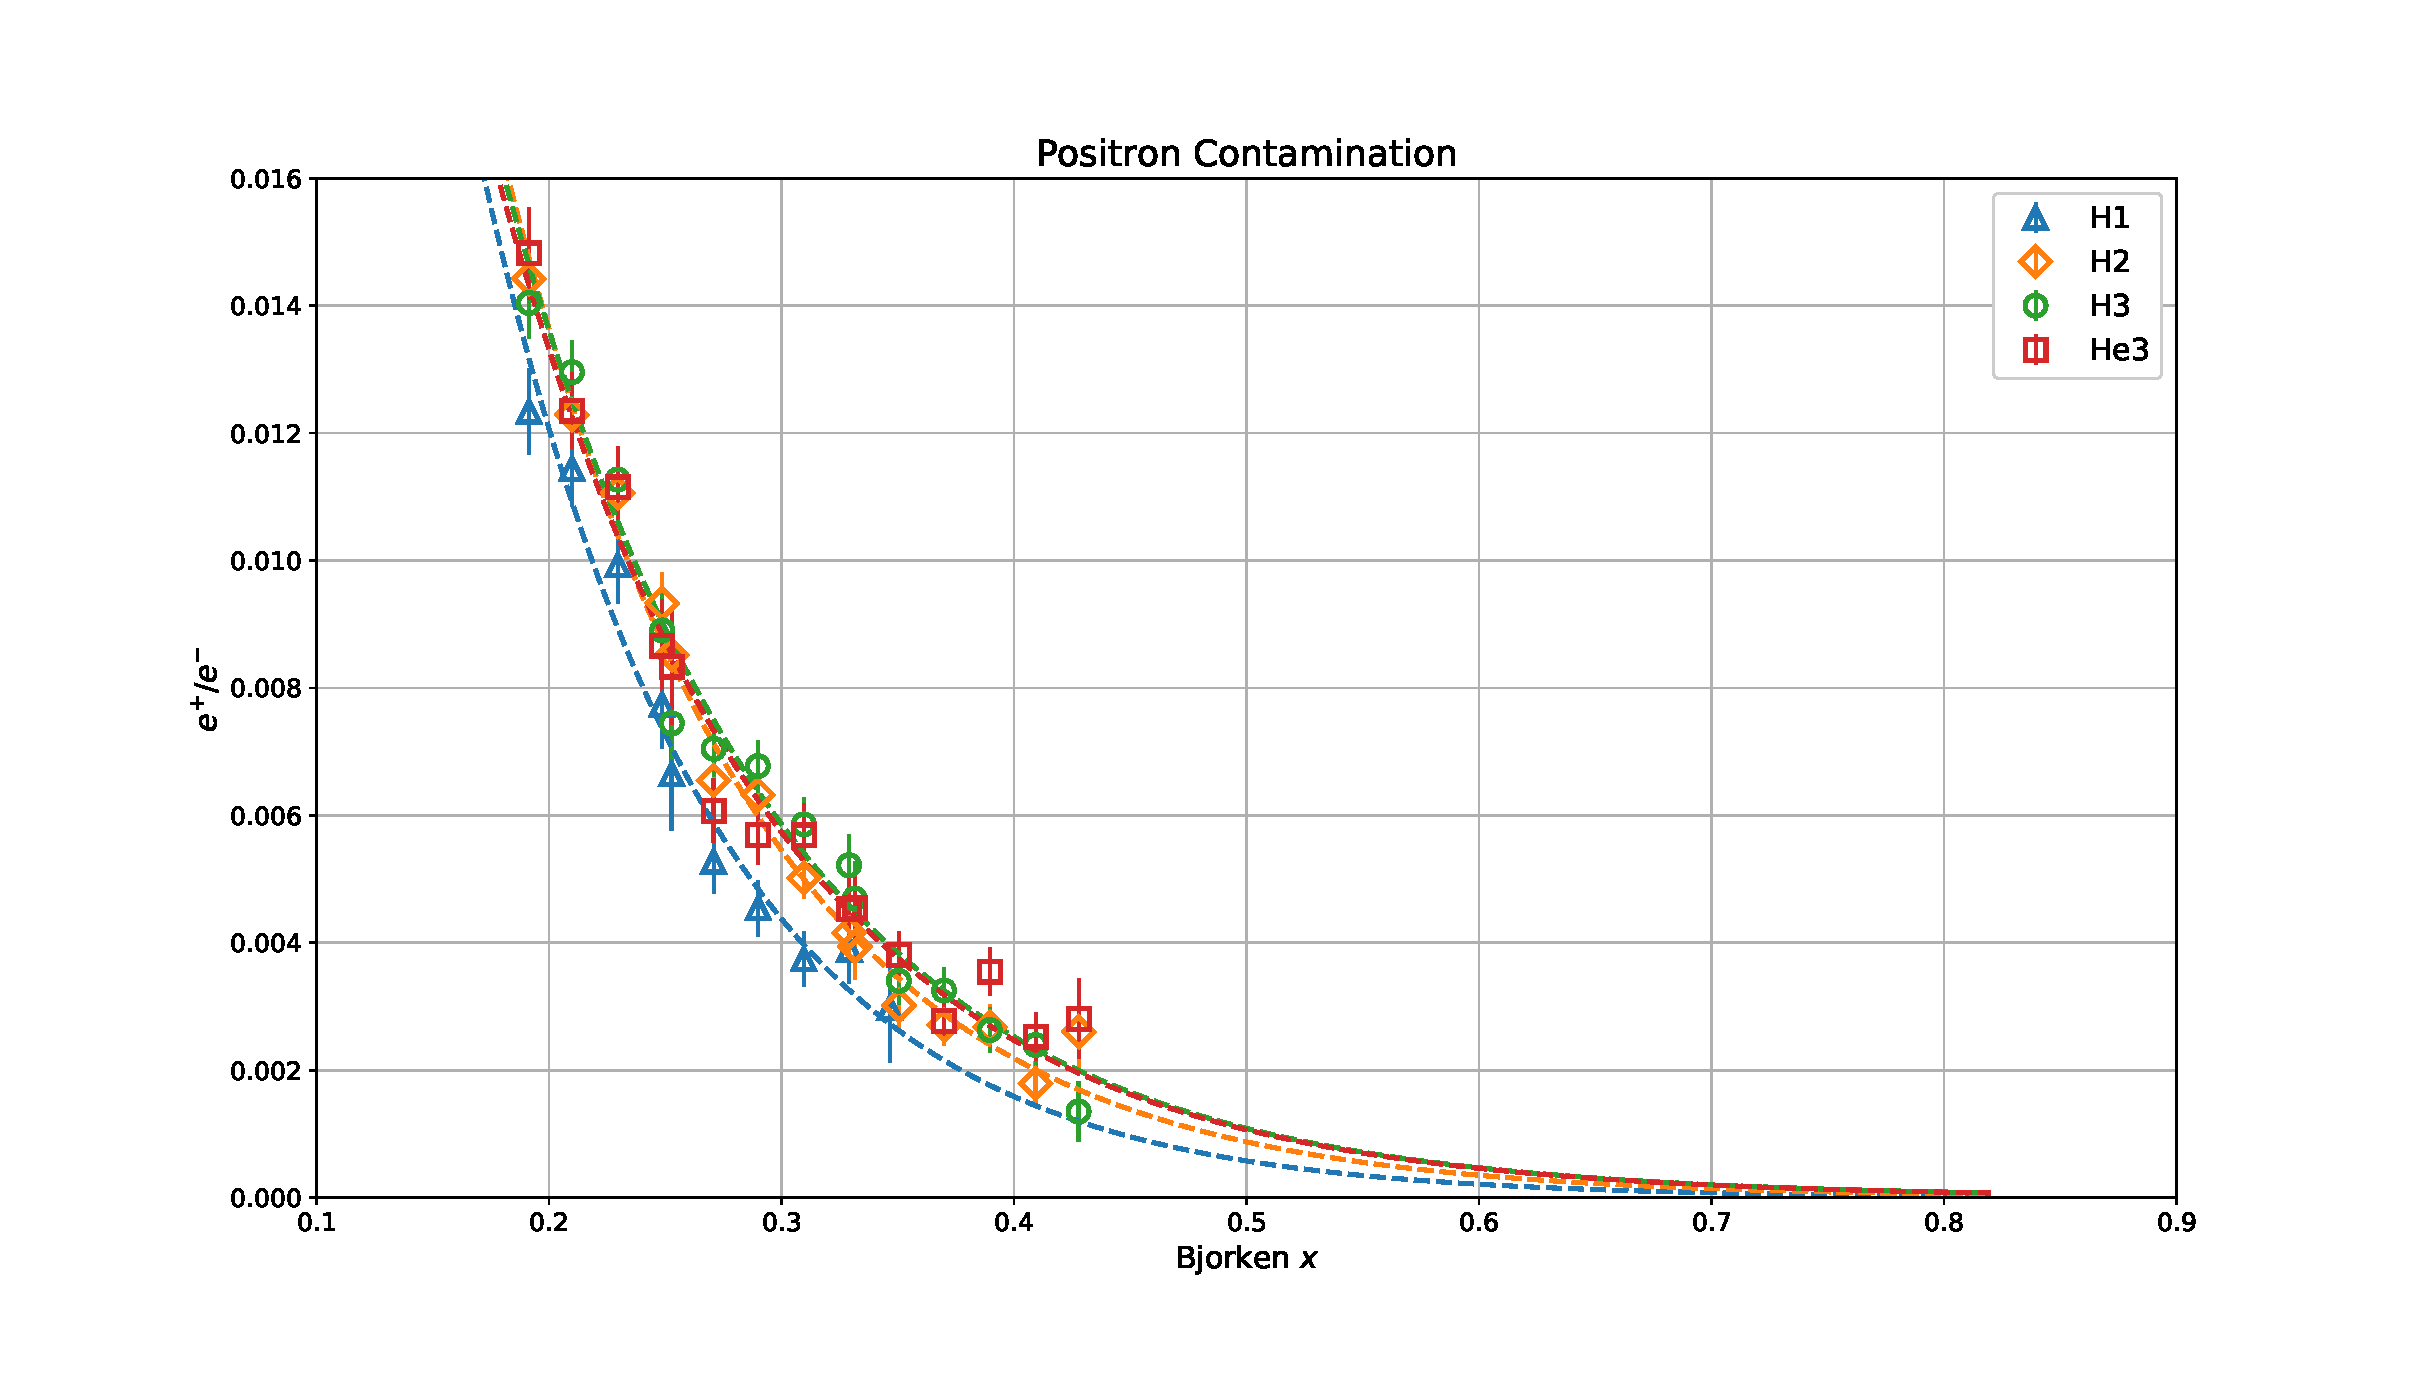
\includegraphics[width=\textwidth]{./analysis/fig/positrons.eps}
	\caption{Charge symmetric background correction}
	\label{fig:positrons}
\end{figure}

\subsection{Computer Deadtime Correction}

Our DAQ unable to continuously record data. While we can probabilistically determine the mean time spacing between events, in the real world events can deviate greatly from these means. Sometimes events will occur that are too close in time for our DAQ to record as the computer has not completed recording the previous event. Deadtime is a function of event rate; when events happen more rapidly, there is a higher chance that events will occur too closely in time to be recorded.

When deadtime is low and the number of recorded events is high, it is a reasonable assumption that the events recorded will accurately reflect the distribution of events in the ``zero-deadtime limit''. In this case correcting for the deadtime is simply done by scaling the number of events by the ``livetime'' of the experiment.

The computer livetime was measured using the Trigger Supervisor and scalers in each HRS. The trigger signals generated from detector signals are copied and sent to both the Trigger Supervisor and a scaler unit. The Trigger Supervisor is subject to the computer deadtime event loss discussed here. The scaler unit, on the other hand, simply increments a register when a trigger signal is received. The ratio of these the number of events recorded by these two systems gives a measure of the livetime of the measurement. The livetime is defined on a run-by-run basis as:

\begin{equation}
DT = \frac{\Sigma \mathrm{Triggers_{TS}}}{\Sigma \mathrm{Triggers_{Scaler}}}
\end{equation}

In an ideal world, the deadtime will be identical for all runs within a kinematic. However, the deadtime is measured on a run-by-run basis and is applied as such in order to account for any deviations from this assumption. The average deadtime for each target in each kinematic is plotted in Figure \ref{fig:deadtime}.

\begin{figure}
	\includegraphics[width=\textwidth]{./analysis/fig/deadtime.eps}
	\caption{Deadtime per kinematic}
	\label{fig:deadtime}
\end{figure}

\subsection{Radiative Corrections}

The Deep Inelastic Cross Sections being studied are the Born approximation of a single-photon exchange. The measurement however, contains contributions from higher order processes that will increase the measured cross section. Using a model, the contributions can be corrected for and removed from the measurement.

The experiment used a software package called $\texttt{T2\_EXTERNALS}$ that calculates both the Born cross section and the radiated cross section for a given target at a kinematic set $(E,E^{\prime} ,\theta )$.

\subsection{Isoscalar Corrections}

\subsection{Bin Centering Corrections}

The cross-section over the width of a bin is not constant. This means that the measurement does not correspond with the true cross section at the center of the bin. Using a model that matches the shape of our data well, the location of the measurement within the bin can be calculated. This is done by calculating the expectation value of the model within that bin and determining the $x$ value corresponding to this value. The expectation value is given by
\begin{equation}
	\langle f_{\rm measured}\rangle = \frac{1}{\Delta x}\int_{x_{\rm low}}^{x_{\rm high}} f\left( x \right) dx,
\end{equation}
where $f$ is a function representing the chosen model. In practice, the $x$ value does not need to be calculated if the data will be reported at the bin center. Rather, the correction is simply the ratio of the model at the bin center. This is written as
\begin{equation}
	\sigma_{\textrm{Bin Centered}} = \frac{f\left(x_{\textrm{Bin Center}}\right)}{\langle f_{\rm measured}\rangle} \sigma_{\rm measured}.
\end{equation}

This correction must be applied to both targets in the ratios. That is, the ratio must be multiplied by the correction to the numerator and divided by the correction to the denominator.\cite{wtsydp}

\subsection{Coulomb Corrections}

Corrections must be made for the effect of the charge of the target on the scattered electron. This interaction causes the $Q^2$ of the event to shift to an effective $Q^2$ value, $Q^2_{\rm eff}$. This conversion is done with the equation
\begin{equation}
	Q^2_{\rm eff} = Q^2 \left(1 + \frac{3Z\alpha\hbar c}{2RE}\right)^{2}.
\end{equation}
In this equation $R$ is the hard-sphere equivalent radius of the nucleus which is defined as $R=\left[\left(\nicefrac{5}{3}\right) \langle r^{2}\rangle\right]^{\nicefrac{1}{2}}$ where $\langle r^2\rangle$ is the root-mean-squared radius of the nucleus.\cite{coulomb}

Using $x=\frac{Q^2}{2M\nu}$, it is clear that a shift in $Q^2$ will result in a proportional shift in $x$. Using a model cross-section, the cross section is calculated at both the nominal $x$ and at $x_{\rm eff}$. As the results have been bin centered, this calculation uses a nominal $x$ at the center of the bin. This will lead to the correction
\begin{equation}
	\sigma_{\textrm{Coulomb Corrected}} = \sigma_{\rm data} \frac{\sigma_{\rm model}\left(x_{\rm eff}\right)}{\sigma_{\rm model}\left(x\right)}.
\end{equation}

This correction must be applied to both targets in the ratios that are calculated.
\subsection{Particle Identification}


\chapter{\bf{The Experiment}}    % Chapter  2
\setcounter{figure}{0}
\setcounter{table}{0}
\setcounter{equation}{0}
\section{The Measurement}
\subsection{What are we measuring}
\subsection{How are we measuring it}
\subsection{Run Plan}

\section{The Apparatus}
\subsection{Hall A HRS Spectrometers}
\subsection{CEBAF Accelerator}

% \chapter{\bf{Chapter 2 Title}    % Chapter  2
%Introductory paragraph of Chapter 2.......
%
%\section{First section Title}
%
%First section text......
%
%
%
%\subsection{First Subsection Title}
%
%
%The cross section for elastic electron scattering from the spin one-half
%$^3$H  nucleus is given, in the one-photon exchange approximation, by:
%\beqn
%{  {d\sigma} \over {d\Omega} } (E,\Theta)  =
%{  {(Z\alpha)^2 E^\prime} \over {4 E^3  \sin^4 \left( {\Theta \over 2} \right)}  }
%\left[ A(Q^2) \cos^2 \left( {\Theta \over 2} \right) +
%B(Q^2) \sin^2 \left( {\Theta \over 2} \right) \right],
%\label{morefequ}
%\eeqn
%where $Z$ is the nuclear charge, $\alpha$ is the fine-structure constant,
%$E$ and $E'$ are the incident and scattered electron energies,
%$\Theta$ is the electron scattering angle, $Q^2 = 4 E E' \sin^2 (\Theta/2)$ is
%minus the squared four-momentum transfer,
%and $A(Q^2)$ and $B(Q^2)$ are the $^3$H elastic structure functions, given in
%terms of the charge and magnetic form factors as:
%\beqn
%{   A(Q^2) = {   { F^2_C(Q^2) +
%(1+\kappa)^2 \tau F^2_M(Q^2) } \over {1 + \tau} }    },
%\label{more1}
%\eeqn
%\beqn
%{ B(Q^2) =  2 \tau (1+\kappa)^2 F^2_M(Q^2) },
%\label{more2}
%\eeqn
%where
%$\tau=Q^2/4M^2$ with $M$ being the mass of the target nucleus, and
%$\kappa$ is the anomalous magnetic moment of the nucleus.
%
%Here is a reference ~\cite{mara} which needs to be defined in the bibliography.tex file first.
%
%
%Here comes a Figure....
%
% \begin{figure}[!htbp]
%  \begin{center}
%    \includegraphics[angle=90, scale=0.65]{./chap2-exp/fig/tritium_past.eps}
%  \end{center}
%  \caption[Tritium Magnetic Form Factor Past Data]{
%    \footnotesize Tritium Mag. Form Factor past data.
%  }
%  \label{fig:TritiumM}
%\end{figure}
%
%Use the label name to refer to  Figure  ~\ref{fig:TritiumM}.
%
%
%\subsection{Second Subsection  Title}
%
%Subsection text..........
%
%
%
%\subsubsection{First Subsubsection}
%
%This is a subsubsection.
%
%
%
%\subsubsection{Second Subsubsection}
%
%This another  subsubsection.

\setcounter{figure}{0}
\setcounter{table}{0}
\setcounter{equation}{0}
\subsection{Raster}
%Put this in order they appear in beamline?
\section{Beamline Components}

The Hall A Beamline has several measurement devices that allow the experimenter to fully understand the beam that is being delivered to the hall. For positioning, there are the Beam Position Monitors and the Harp. For beamspot sizing, there is the raster. For current and charge measurements, there are the Beam Current Monitors.

\subsection{Beam Position Monitors}

The Beam Position Monitors (BPMs) are a pair of measurement devices that consist of four sensing wires. By calibrating the signal received from each wire, the experimenter can reconstruct the position of the beam as it passed the BPM. Using both BPMs in conjunction allows the experimenter to determine the beam trajectory and where the electrons are incident on the target.

The BPMs are calibrated using a Harp fork. The Harp consists of three wires that are introduced sequentially into the path of the beam using a stepper motor. When the beam is incident on a wire, a charge is induced. By determining when each wire is struck by the beam, the experimenter can very accurately determine the position of the beam. This is an invasive measurement.

\subsection{Raster}
\begin{figure}
	\includegraphics[width=\linewidth]{./chap2-exp/fig/raster_pic.jpg}
	\caption{The Hall A raster consists of four dipole magnets on the beamline}
	\label{fig:raster}
\end{figure}

The raster is a beamline apparatus in Hall A for spreading the beam onto the target, rather than being at a single point. This is done to prevent localized heating of the target. The raster consists of four dipole magnets, two for steering in the x-direction and two for steering in the y-direction.

Each raster magnet is powered by a triangle wave of different frequencies to minimize harmonics. The horizontal rasters are set to 24.5 kHz and the vertical rasters are set to 25 kHz. When running properly, the x-direction magnets will be synced and the y-direction magnets will be synced. This syncing ensures that the magnets are always working together to create the desired beam spread.

\begin{figure}
	\includegraphics[width=\linewidth]{./chap2-exp/fig/raster_sync.png}
	\caption{The X and Y raster pairs are each synced to produce the maximum kick. The X and Y directions are uncorrelated so that the beam travels uniformly over the target.}
	\label{fig:raster}
\end{figure}

\subsection{Beam Current Monitors}


\chapter{\bf{Analysis}}    % Chapter  3
\setcounter{figure}{0}
\setcounter{table}{0}
\setcounter{equation}{0}
\section{Yield Calculation}

The MARATHON experiment measured cross section ratios. This method allows us to cancel many systematics that would otherwise plague a full cross section analysis. By taking data for each target at the same kinematics, acceptance effects are identical. This data taking technique means that with reasonable acceptance cuts, a ratio of target yields is wholly equivalent to the ratio of cross sections.

To calculate the yield we use a simple equation:

\begin{equation}
	\text{Yield} = \frac{\text{Counts}}{\text{Scattering Centers} \cdot \text{Livetime}} \cdot \text{Corrections}
\end{equation}

The yield is binned in Bjorken $x$. This chapter will explain the cuts and corrections that go into this calculation.

\section{Calibration}
\subsection{Raster Calibration}
The raster is calibrated by defining a line that maps the raster current to positions at each BPM and the target. To do this, the slope and intercept of this line had to be determined. The slope corresponds to the conversion of raster current to position displacement. The intercept is then determined from the central position that the beam is displaced from. This section will be a general presentation of the techniques used to calibrate the raster. For a more in-depth discussion of how the raster was calibrated, see Appendix \ref{raster_appendix}.

For the horizontal raster, this was done by optimizing the reconstructed z-vertex on the target. When properly calibrated, there should be no correlation between the horizontal raster and the z-vertex. Linear interpolation between two ``bad'' calibrations is a simple way to determine the correct calibration slope.

The veritcal raster could be calibrated in a similar way by minimizing the correlation between the vertical raster and a known momentum phenomena (i.e. a $W^2$ peak). Unfortunately, such a feature does not exist within the kinematics of MARATHON data. The vertical calibration was determined using the carbon hole target. The hole is known to be $2mm$ diameter. By using the raster data, the hole can be fit in order to determine the vertical calibration slope.

The intercepts are determined by looking at the mean BPM position readings and projecting these to the target. This position will correspond to the mean value of the rasters as well. Using the beam position, raster current, and calibration slope the calibration intercept can easily be determined.


\section{Analysis}
\section{Corrections}

When analyzing the data, there are several corrections that need to be made. These are due to various physical or systematic effects that took place during the experiment. These effects have been studied in order to determine a ``correction factor'' that can be applied to the data.

\subsection{Target Boiling}
\label{sec:boiling}

When the beam is incident on the target, it deposits heat into the gas. This causes a density fluctuation of the gas referred to as ``target boiling''. The target does not actually boil, however that is the standard nomenclature for a density fluctuation in a gas target. When the density of the target changes, it changes the effective target thickness as seen by the beam. When the target thickness changes, there is a changed number of scattering centers which will lead to a change in the number of electrons recorded. Specifically, heating will decrease the target density which will decrease the number of scattered electrons.

The density changes are a function of the current on the target. Each run is taken at a single current so that the correction can be applied run by run. The correction is approximately linear for small deviations in current. A study of the effect during beam ramping found that the density settles very quickly. This means that so long as we cut events that occur with the beam off, it is unnecessary to take into account the beam ramping when correcting for this effect.

To determine the correction, a dedicated set of runs was taken with the Left HRS spectrometer at $16.8\degree$ and 3.1 GeV. At this kinematic, several data runs were recorded with varying current between them. Each of these runs were analyzed with the standard data cuts to determine the yield. This allows for the yield to be determined as a function of beam current.

Now that the yields have been determined as a function of beam current, they can be plotted and fit. The data is fit with a quadratic polynomial. This fit is constrained to require no correction (a correction factor of 1) at zero current. This is because the density must be the nominal fill density when there is no beam heating. During analysis the average current is calculated for a run (ignoring beam trips). The average current is then used to calculate the target density correction with the fit function. The correction is then applied on a run-by-run basis by multiplying the number of scattering centers by this correction factor (or equivalently dividing the yield by the correction factor). Figure \ref{fig:boilcor} shows the correction factors for each target.\cite{boiling}

\begin{figure}
	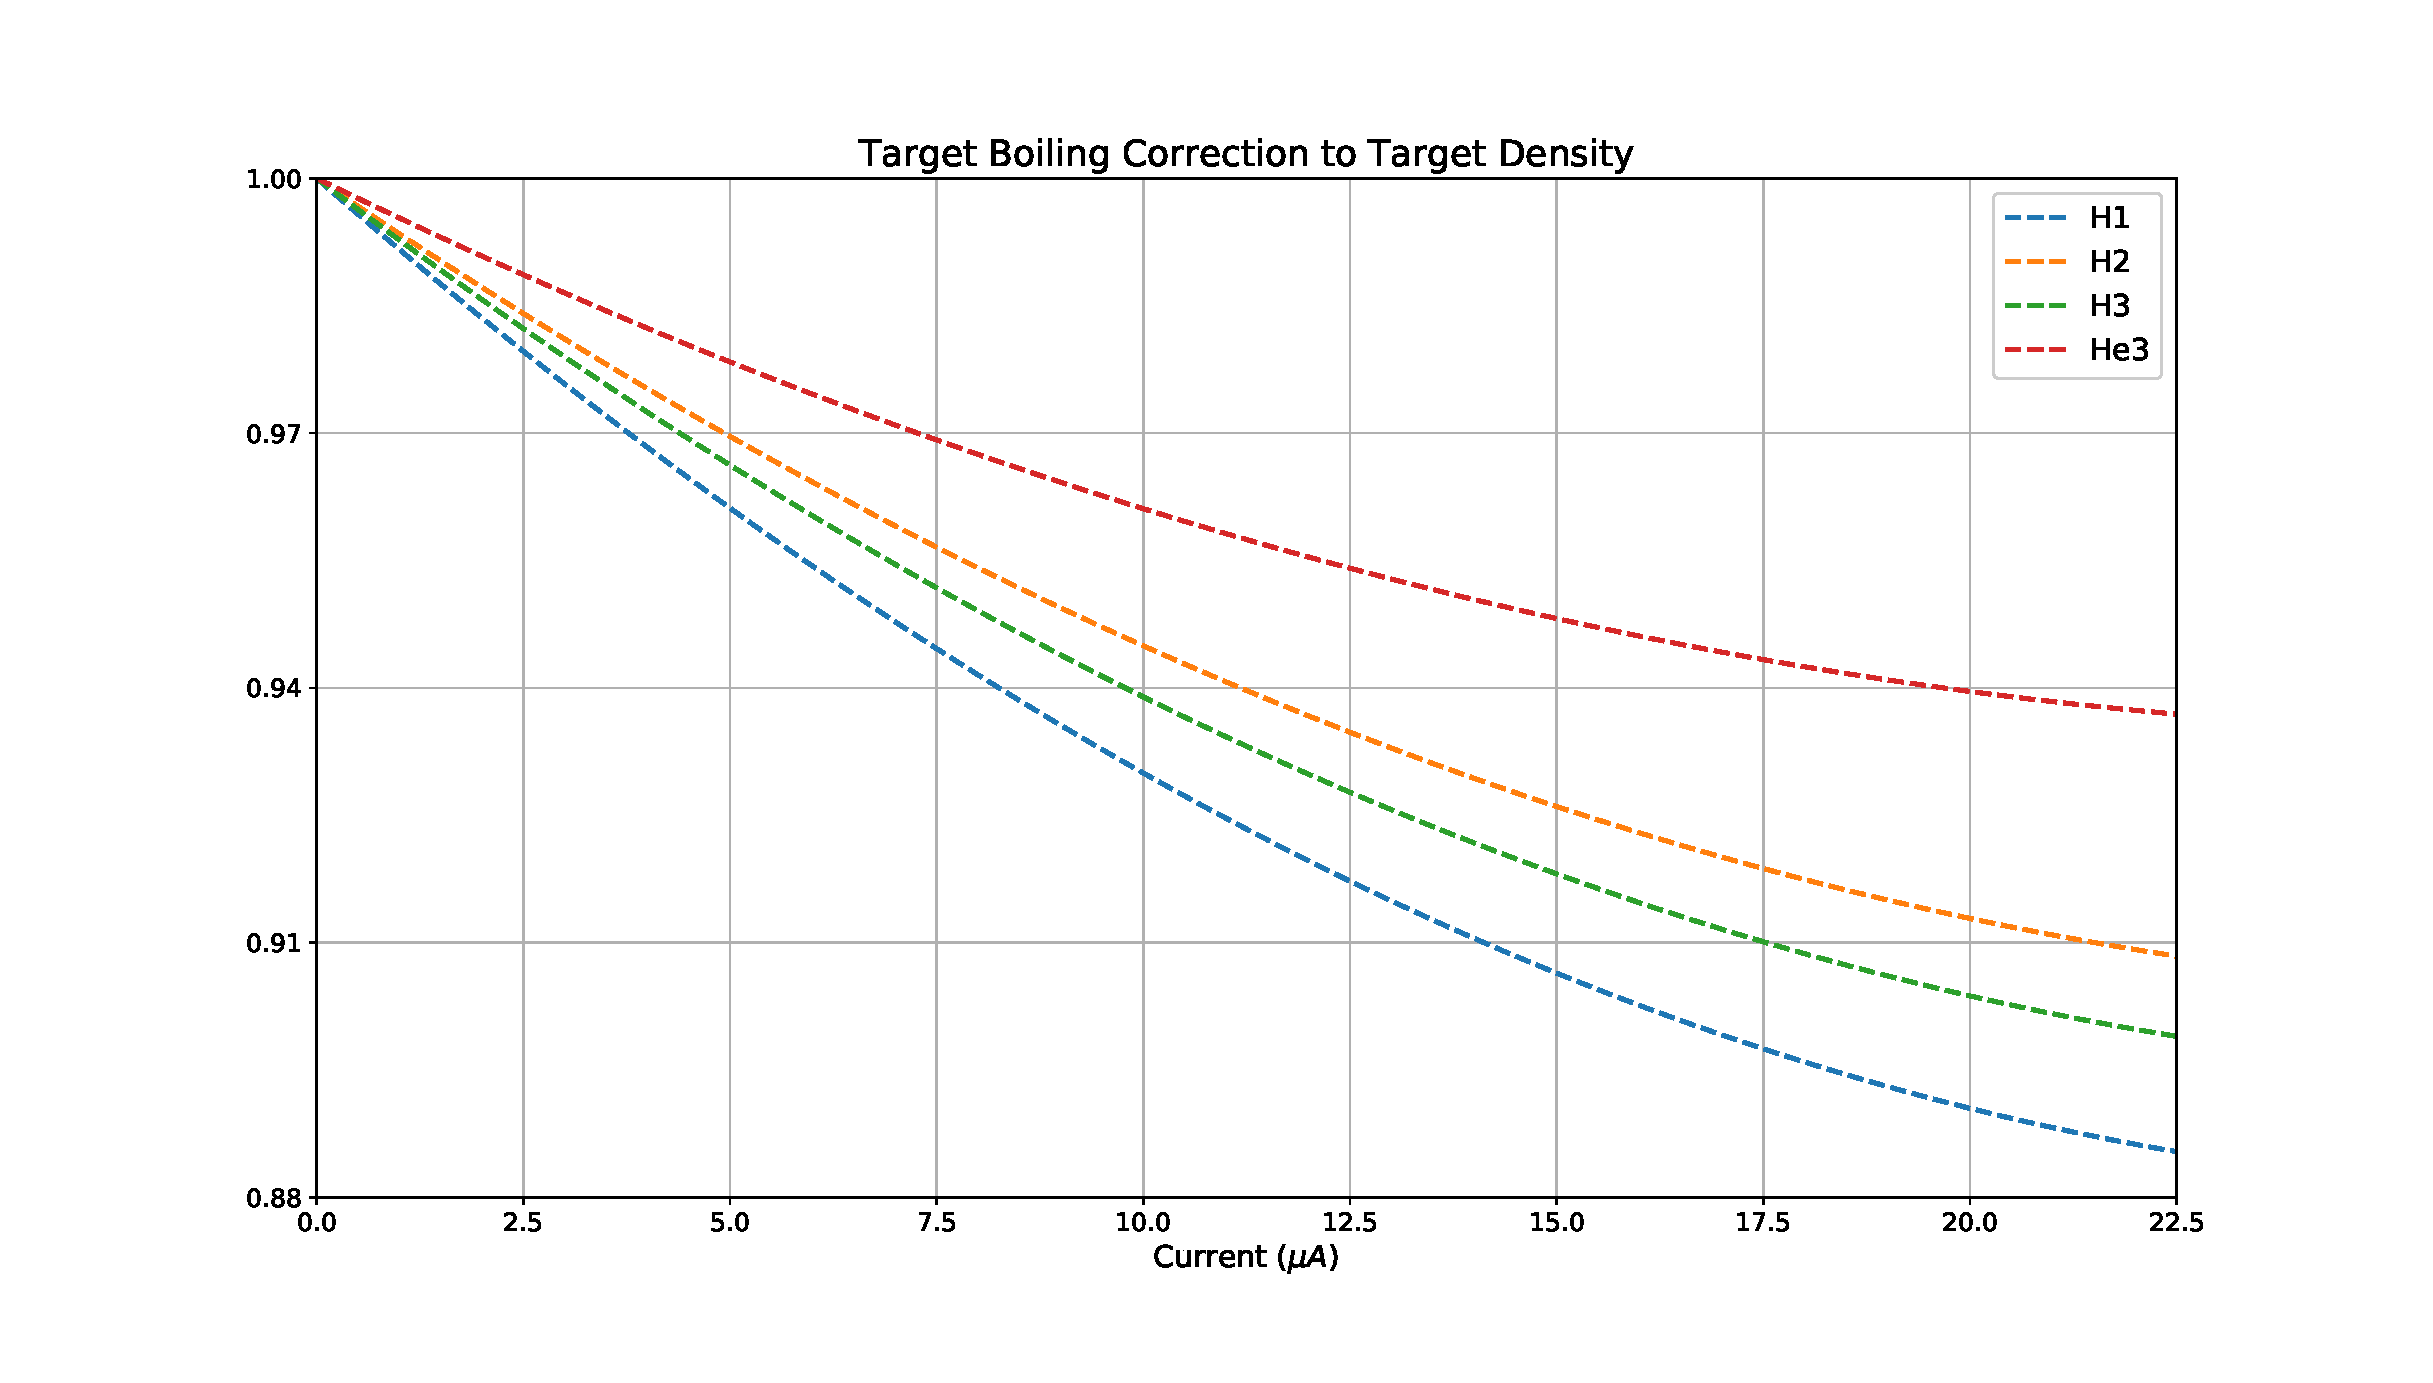
\includegraphics[width=\textwidth]{./analysis/fig/boil_cor.eps}
	\caption{Beam heating effects are manifested as a multiplicative correction to the target density}
	\label{fig:boilcor}
\end{figure}

%\begin{figure}
%	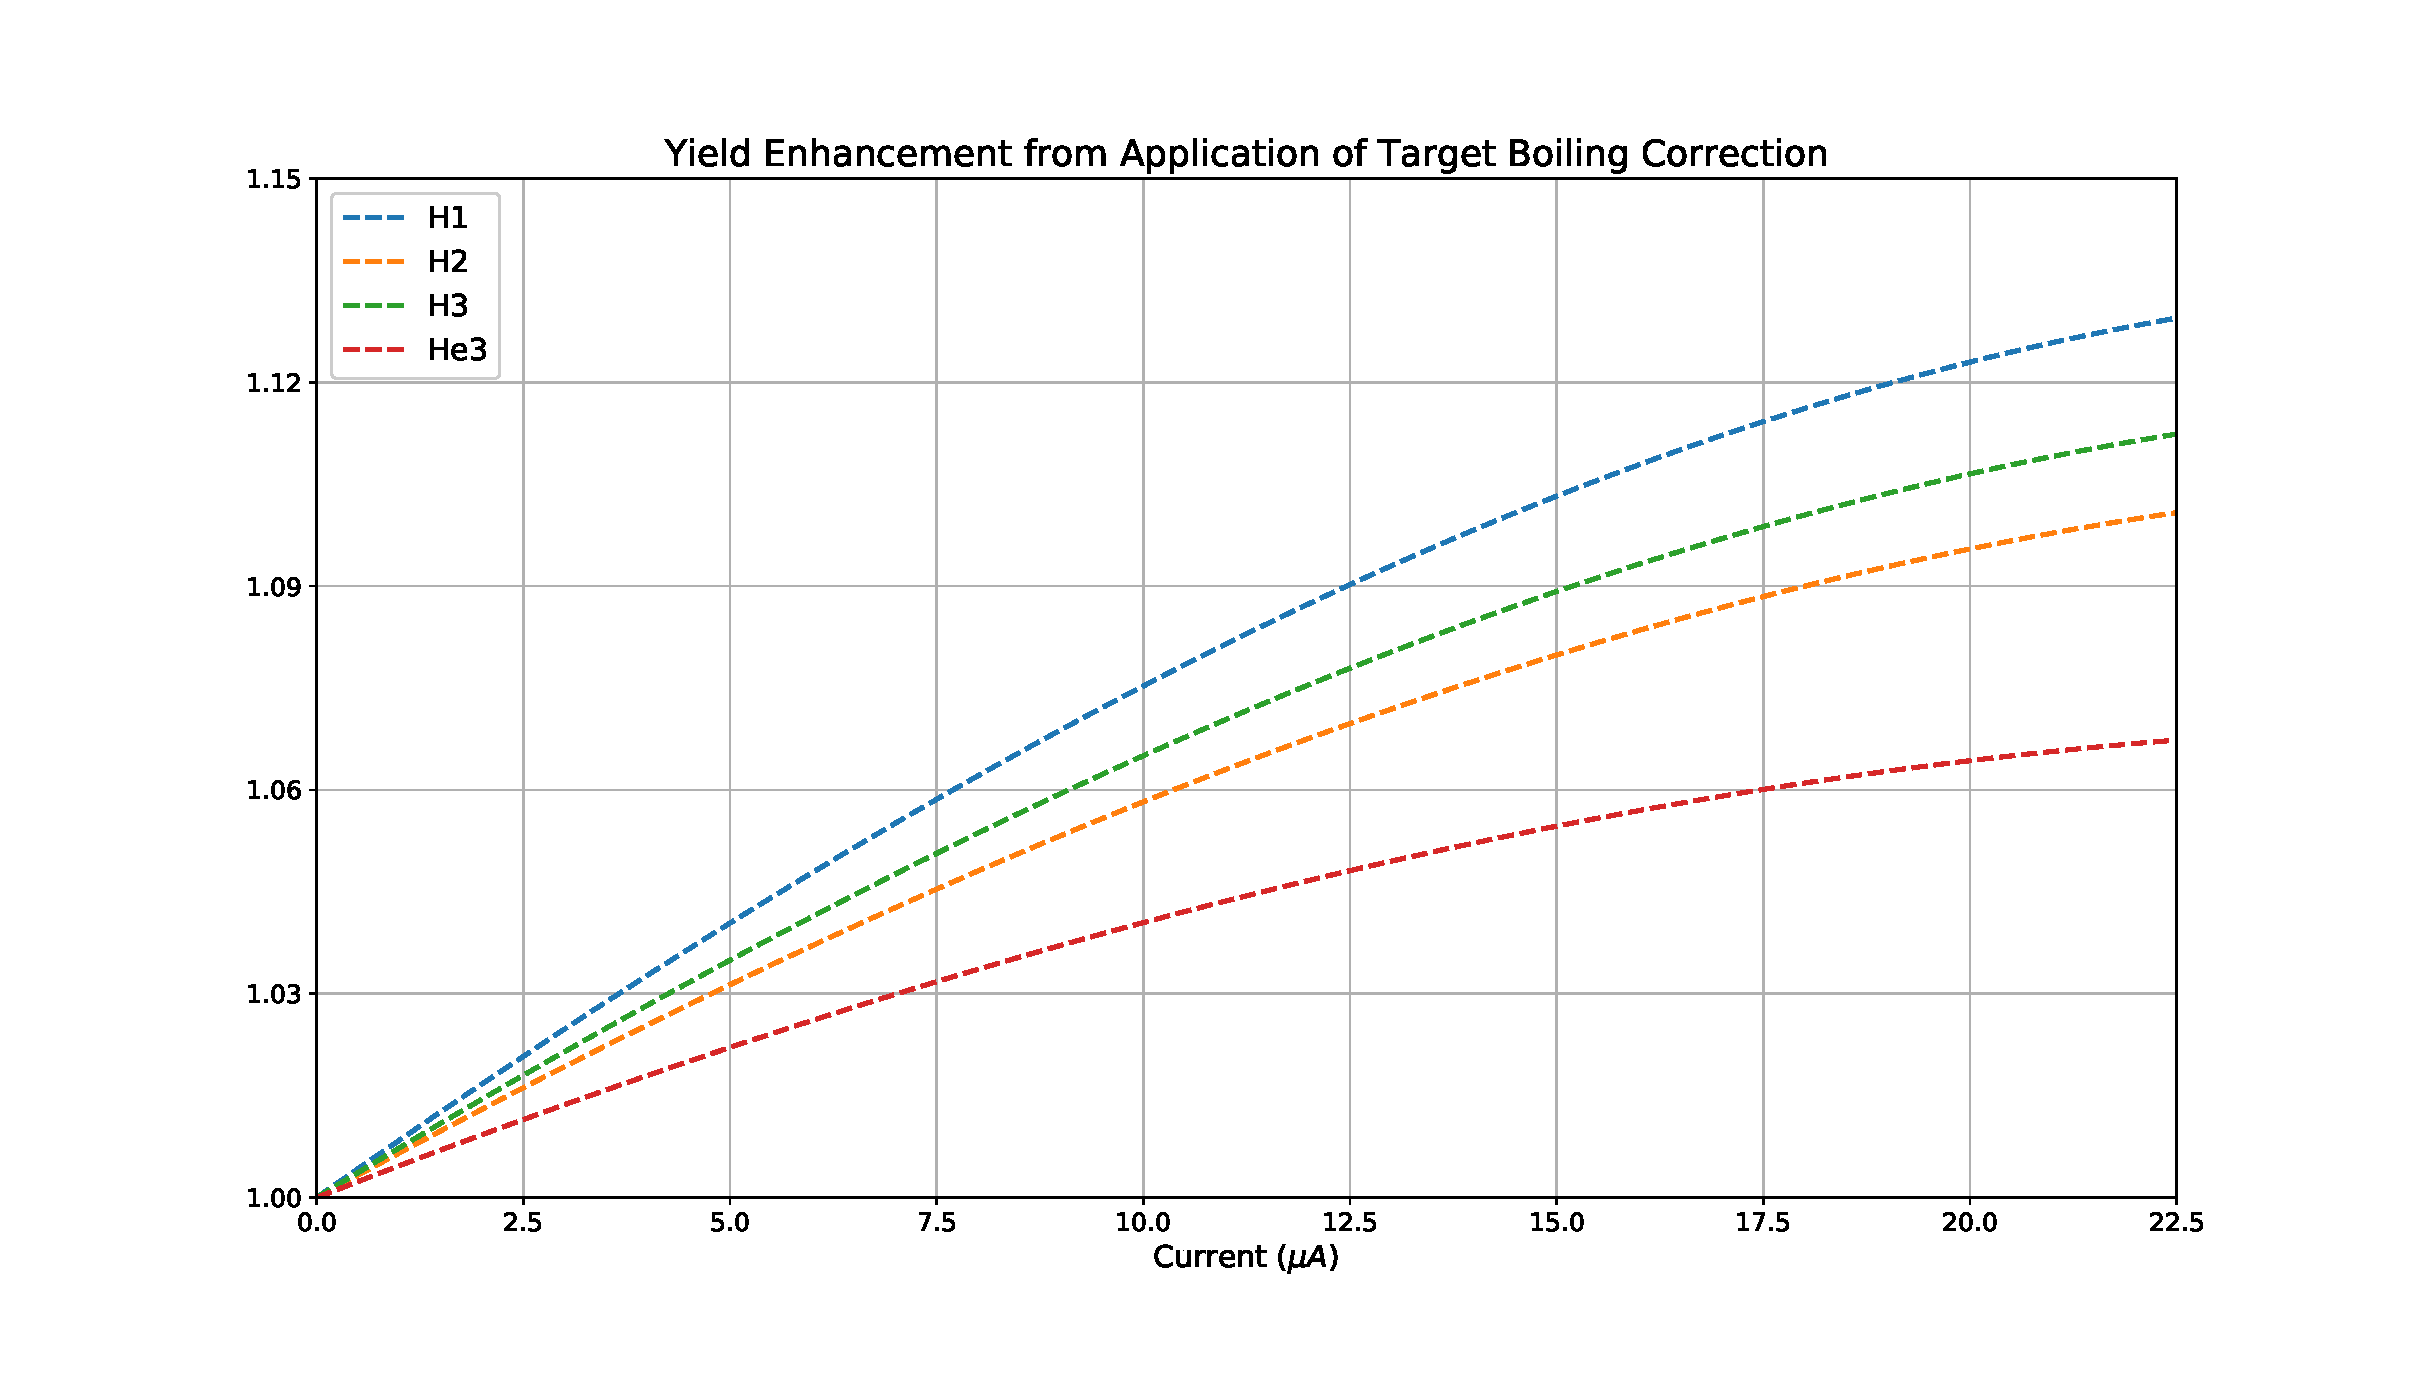
\includegraphics[width=\textwidth]{./analysis/fig/boil_yield_cor.eps}
%	\caption{Target density corrections cause a multiplicative enhancement to the yield}
%	\label{fig:boilyieldcor}
%\end{figure}

\subsection{Target Endcap Contamination}
\label{sec:ecc}

The gas targets used in this experiment are housed in aluminum cells as described in Section \ref{sec:gas_cell}. The thickness of the aluminum greatly exceeds the thickness of the gas and will contribute background that can survive the cuts placed on the data. By quantifying this contribution, the events that originate from the cell endcaps can be subtracted from the final results.

To determine this contribution, the empty cell is used. The empty cell, being an exact replica of the gas target cells with a vacuum inside, allows us to approximately isolate the contribution of the cell walls to the data. The empty cell and the target being studied are compared by calculating the yields on a kinematic-by-kinematic basis and normalizing them by charge and endcap thickness.

The normalization to the endcaps for each target must be done in two parts. This is because each endcap is not the same thickness. When calculating the yield for a target, it is assumed that any contamination upstream (downstream) of the center of the target must originate from the upstream (downstream) endcap. The two halves are then combined to arrive at the endcap thickness normalized yield. This yield calculation only has livetime corrections applied. All cuts are applied except for target length, which is adjusted to only include events upstream (downstream) of the center of the target.

The data for the target being studied and the normalized empty target are then binned in Bjorken $x$. Dividing the empty cell data by the gas target data then gives an approximation of the fractional contribution of the cell walls to the electron data. As this correction is applied to the final results, the contamination corrections for the targets are divided by each other to create the correction to the target ratios. These results are then fit with the functional form $1\pm e^{Ax+B}$. The choice of adding or subtracting the exponential is done by determining if the correction is greater or smaller than 1. The fit function and the covariance matrix of the fit are used to apply the correction to the final results as well as determine the uncertainty contribution of this correction.

\subsection{Charge Symmetric Background Subtraction}

As an inclusive scattering experiment, we are particularly susceptible to background from charge symmetric processes from the target. That is events which involved the production of both an electron and a positron, rather than the electron simply scattering. To study this, the polarity of the LHRS was reversed so that positively charge particles are directed into the detectors rather than negatively charged particles. With this setting, a number of runs were taken in kinematics 0 through 5. These runs were taken with all targets, just as the electron data was taken. This allows for a measurement of the positron yield which corresponds to a measure of the charge symmetric background.

This measurement allows us to determine the proportion of electrons that originated from pair production. Applying the same cuts and as the electron data allows us to determine the charge normalized positron yield. Unlike in the electron analysis, it was noted that there was significant pion contamination in the positron data. This pion contamination had to be subtracted in order to get an accurate calculation of the positron yield. This is achieved by fitting the main pion peak and the subtracting the tail of the fit which survives the cuts applied from the positron data.

The charge normalized positron yields over these kinematics are then combined (using the same methods as the electron yield) and binned in Bjorken $x$. This was then divided by the charge normalized electron yield. This is a fractional measure of the charge normalized background contamination. The ratio is then fit with an exponential of the form $e^{Ax + B}$, where $A$ and $B$ are the fit parameters. These fits are shown in in Figure \ref{fig:positrons}.

This correction is applied to the final yield ratio results. Both the numerator and denominator must have the charge symmetric background subtracted. Each target yield in the ratio is scaled by $1 - \left(\textrm{Charge Symmetric Background Fit}\right)$. For each bin, the fit is calculated at the bin center.

\begin{figure}
	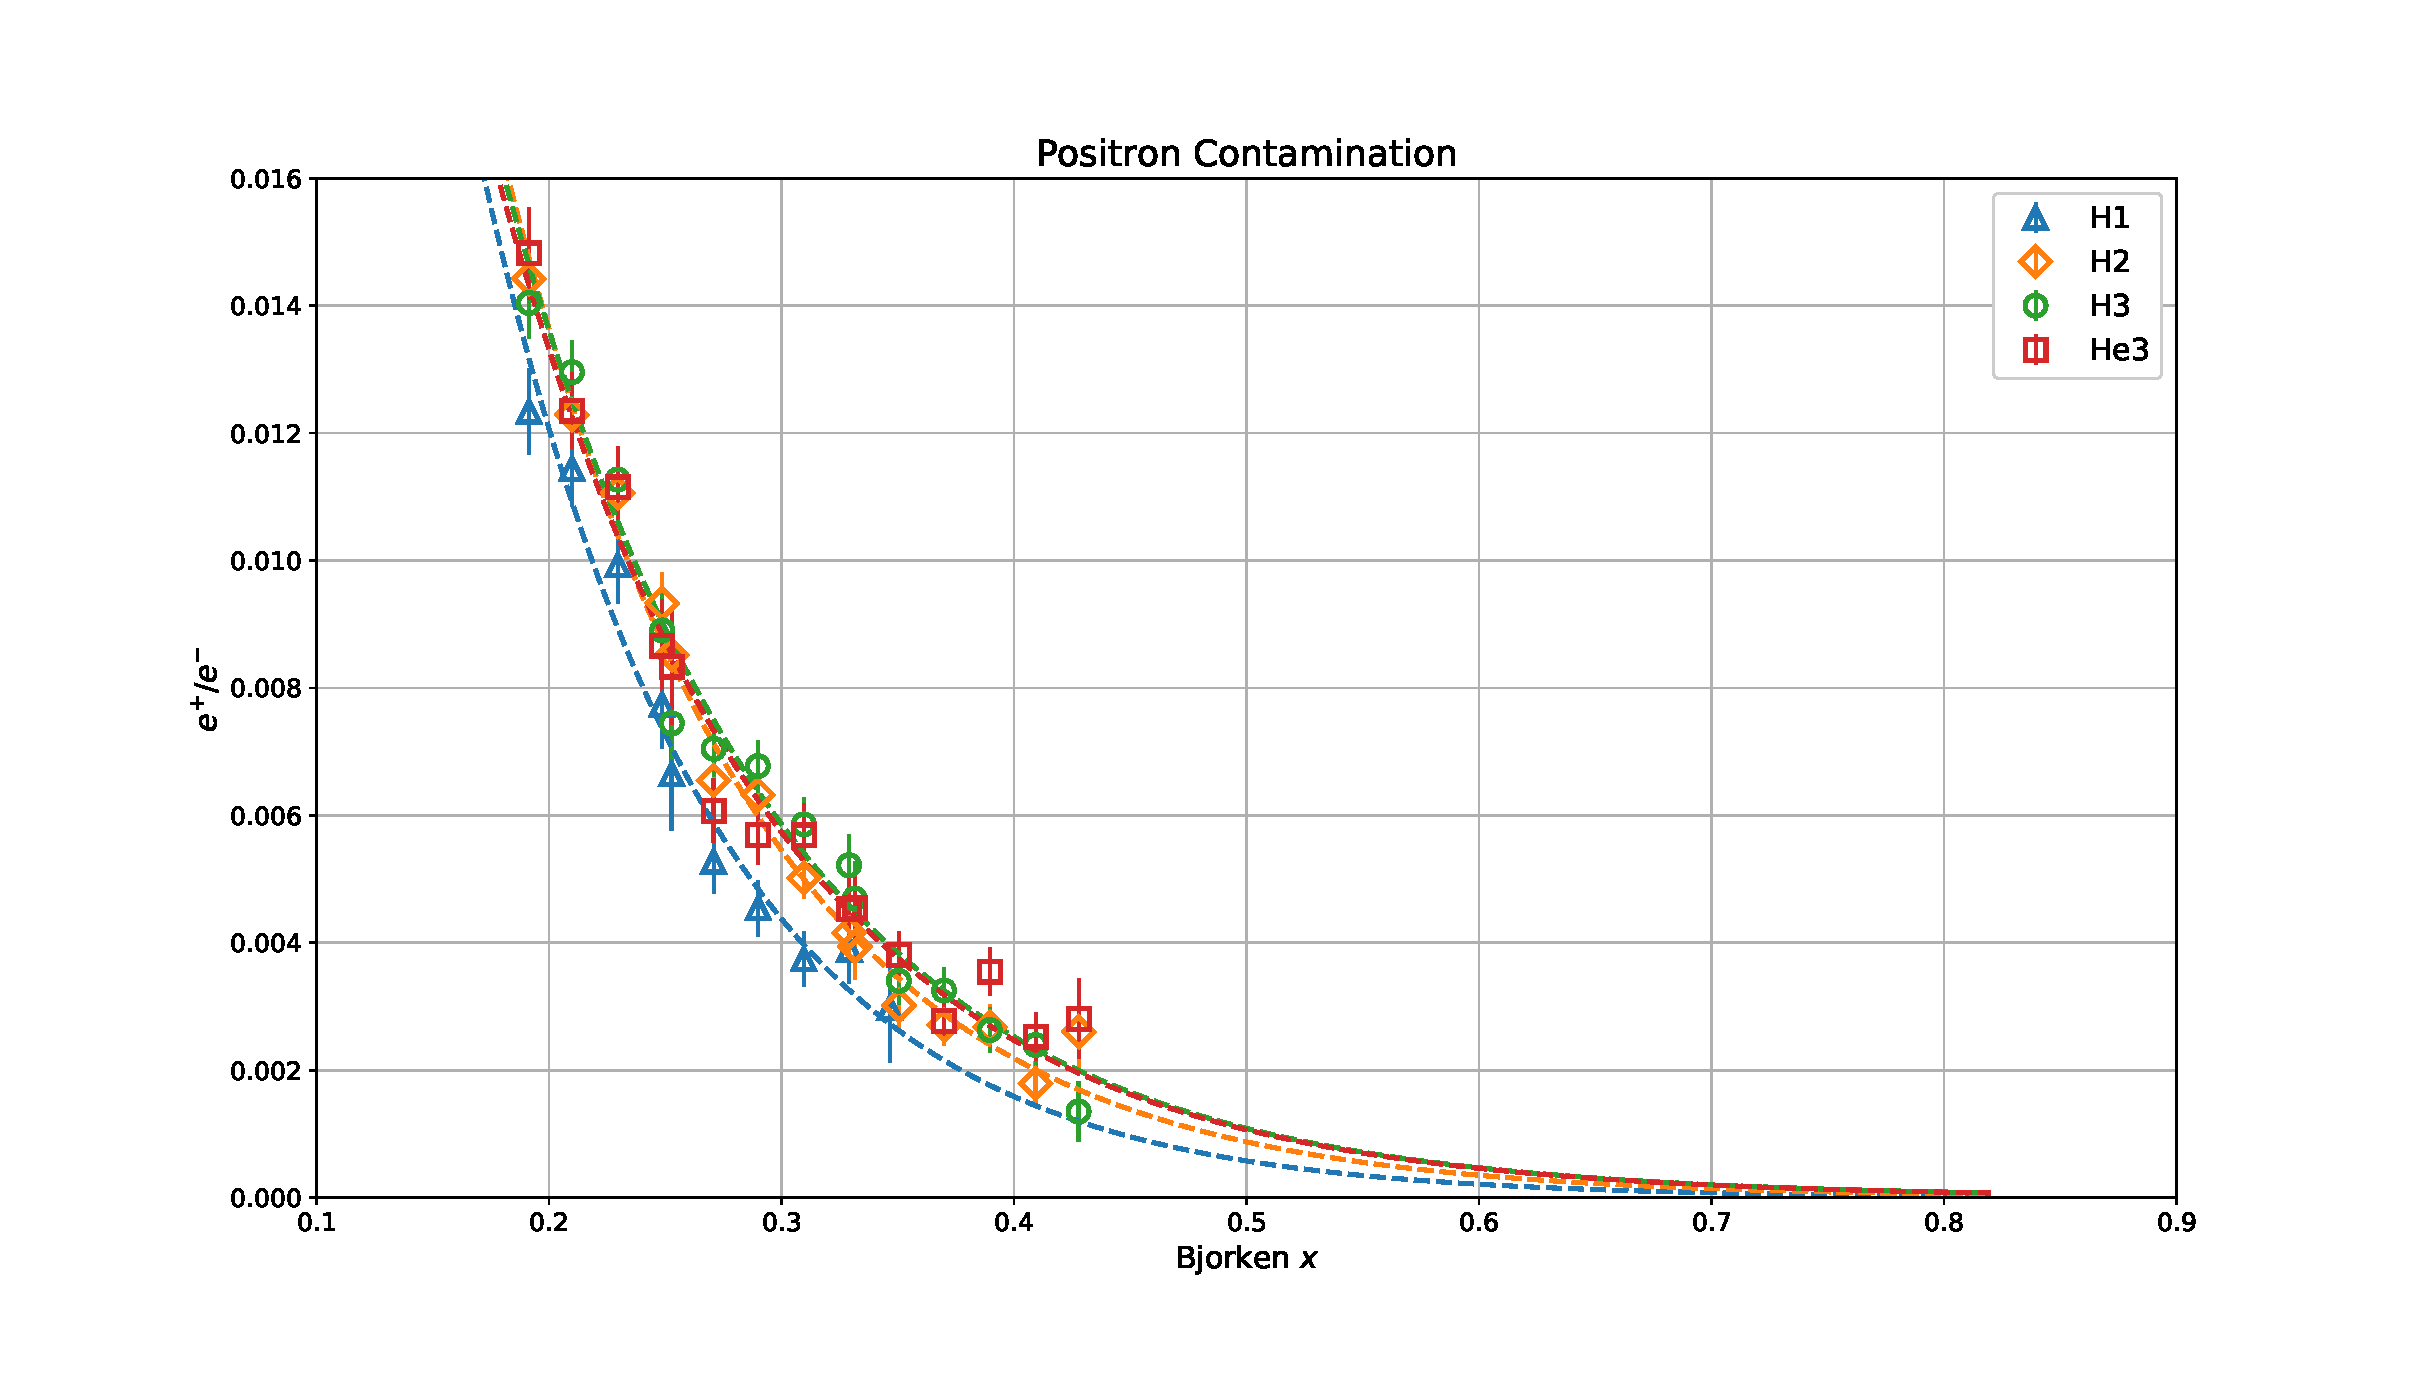
\includegraphics[width=\textwidth]{./analysis/fig/positrons.eps}
	\caption{Charge symmetric background correction}
	\label{fig:positrons}
\end{figure}

\subsection{Computer Deadtime Correction}

Our DAQ unable to continuously record data. While we can probabilistically determine the mean time spacing between events, in the real world events can deviate greatly from these means. Sometimes events will occur that are too close in time for our DAQ to record as the computer has not completed recording the previous event. Deadtime is a function of event rate; when events happen more rapidly, there is a higher chance that events will occur too closely in time to be recorded.

When deadtime is low and the number of recorded events is high, it is a reasonable assumption that the events recorded will accurately reflect the distribution of events in the ``zero-deadtime limit''. In this case correcting for the deadtime is simply done by scaling the number of events by the ``livetime'' of the experiment.

The computer livetime was measured using the Trigger Supervisor and scalers in each HRS. The trigger signals generated from detector signals are copied and sent to both the Trigger Supervisor and a scaler unit. The Trigger Supervisor is subject to the computer deadtime event loss discussed here. The scaler unit, on the other hand, simply increments a register when a trigger signal is received. The ratio of these the number of events recorded by these two systems gives a measure of the livetime of the measurement. The livetime is defined on a run-by-run basis as:

\begin{equation}
DT = \frac{\Sigma \mathrm{Triggers_{TS}}}{\Sigma \mathrm{Triggers_{Scaler}}}
\end{equation}

In an ideal world, the deadtime will be identical for all runs within a kinematic. However, the deadtime is measured on a run-by-run basis and is applied as such in order to account for any deviations from this assumption. The average deadtime for each target in each kinematic is plotted in Figure \ref{fig:deadtime}.

\begin{figure}
	\includegraphics[width=\textwidth]{./analysis/fig/deadtime.eps}
	\caption{Deadtime per kinematic}
	\label{fig:deadtime}
\end{figure}

\subsection{Radiative Corrections}

The Deep Inelastic Cross Sections being studied are the Born approximation of a single-photon exchange. The measurement however, contains contributions from higher order processes that will increase the measured cross section. Using a model, the contributions can be corrected for and removed from the measurement.

The experiment used a software package called $\texttt{T2\_EXTERNALS}$ that calculates both the Born cross section and the radiated cross section for a given target at a kinematic set $(E,E^{\prime} ,\theta )$.

\subsection{Isoscalar Corrections}

\subsection{Bin Centering Corrections}

The cross-section over the width of a bin is not constant. This means that the measurement does not correspond with the true cross section at the center of the bin. Using a model that matches the shape of our data well, the location of the measurement within the bin can be calculated. This is done by calculating the expectation value of the model within that bin and determining the $x$ value corresponding to this value. The expectation value is given by
\begin{equation}
	\langle f_{\rm measured}\rangle = \frac{1}{\Delta x}\int_{x_{\rm low}}^{x_{\rm high}} f\left( x \right) dx,
\end{equation}
where $f$ is a function representing the chosen model. In practice, the $x$ value does not need to be calculated if the data will be reported at the bin center. Rather, the correction is simply the ratio of the model at the bin center. This is written as
\begin{equation}
	\sigma_{\textrm{Bin Centered}} = \frac{f\left(x_{\textrm{Bin Center}}\right)}{\langle f_{\rm measured}\rangle} \sigma_{\rm measured}.
\end{equation}

This correction must be applied to both targets in the ratios. That is, the ratio must be multiplied by the correction to the numerator and divided by the correction to the denominator.\cite{wtsydp}

\subsection{Coulomb Corrections}

Corrections must be made for the effect of the charge of the target on the scattered electron. This interaction causes the $Q^2$ of the event to shift to an effective $Q^2$ value, $Q^2_{\rm eff}$. This conversion is done with the equation
\begin{equation}
	Q^2_{\rm eff} = Q^2 \left(1 + \frac{3Z\alpha\hbar c}{2RE}\right)^{2}.
\end{equation}
In this equation $R$ is the hard-sphere equivalent radius of the nucleus which is defined as $R=\left[\left(\nicefrac{5}{3}\right) \langle r^{2}\rangle\right]^{\nicefrac{1}{2}}$ where $\langle r^2\rangle$ is the root-mean-squared radius of the nucleus.\cite{coulomb}

Using $x=\frac{Q^2}{2M\nu}$, it is clear that a shift in $Q^2$ will result in a proportional shift in $x$. Using a model cross-section, the cross section is calculated at both the nominal $x$ and at $x_{\rm eff}$. As the results have been bin centered, this calculation uses a nominal $x$ at the center of the bin. This will lead to the correction
\begin{equation}
	\sigma_{\textrm{Coulomb Corrected}} = \sigma_{\rm data} \frac{\sigma_{\rm model}\left(x_{\rm eff}\right)}{\sigma_{\rm model}\left(x\right)}.
\end{equation}

This correction must be applied to both targets in the ratios that are calculated.
\subsection{Particle Identification}


\chapter{\bf{Results}}    % Chapter  4
\setcounter{figure}{0}
\setcounter{table}{0}
\setcounter{equation}{0}
%\section{Title of First section}
%
%
%\subsection{First subsection}
%
%Here is a Table....
%
%\begin{table}[ht!]
%\caption{Forward Electron Scattering Run Plan}
%\begin{center}
%\begin{tabular}{cccccccc}
%%\multicolumn {7} {c}  {\bf TABLE 4} \\
%\multicolumn {7} {c}  {\bf FORWARD ELECTRON SCATTERING RUN PLAN } \\
%\multicolumn {7} {c}  { } \\ \hline
%$Q^2$  &  $F_C$  & $F_M$ &Cross Section & Time  & Counts & $\Delta F_C$ \\
% (fm$^{-2}$)  &  &  & (cm$^2$/sr) & (hr)  &  & ($\pm\%$) \\ \hline
%    &                     &                     &                           &     &     \\
%12.90 & 3.0$\times 10^{-4}$ & 8.0$\times 10^{-3}$ & 2.7$\times 10^{-34}$ & 1.2 & 12240 & NM  \\
%15.50 & 3.0$\times 10^{-3}$ & 3.4$\times 10^{-3}$ & 5.9$\times 10^{-35}$ & 4.8 & 10800 & 13 \\
%17.50 & 3.5$\times 10^{-3}$ & 1.8$\times 10^{-3}$ & 3.0$\times 10^{-35}$ & 1.2 & 1380  & 9.5 \\
%20.00 & 3.3$\times 10^{-3}$ & 7.0$\times 10^{-4}$ & 1.5$\times 10^{-35}$ & 2.4 & 1360  & 4.1 \\
%22.80 & 2.8$\times 10^{-3}$ & 6.0$\times 10^{-5}$ & 1.4$\times 10^{-35}$ & 1.2 & 630   & 5.4 \\
%26.00 & 2.2$\times 10^{-3}$ & 3.0$\times 10^{-4}$ & 6.4$\times 10^{-36}$ & 4.8 & 1175  & 3.1 \\
%28.00 & 1.8$\times 10^{-3}$ & 4.7$\times 10^{-4}$ & 4.4$\times 10^{-36}$ & 2.4 & 395   & 5.2 \\
%31.50 & 1.3$\times 10^{-3}$ & 5.0$\times 10^{-4}$ & 2.2$\times 10^{-36}$ & 12  & 990   & 11 \\
%35.00 & 9.0$\times 10^{-4}$ & 4.2$\times 10^{-4}$ & 9.9$\times 10^{-37}$ & 9.6 & 360   & 17 \\
%39.25 & 5.5$\times 10^{-4}$ & 3.0$\times 10^{-4}$ & 3.5$\times 10^{-37}$ & 12  & 160   & 25 \\
%43.00 & 3.2$\times 10^{-4}$ & 1.9$\times 10^{-4}$ & 1.1$\times 10^{-37}$ & 19  & 83    & 35 \\
%47.50 & 2.0$\times 10^{-4}$ & 1.1$\times 10^{-4}$ & 3.4$\times 10^{-38}$ & 12  & 16    & NM \\
%Total      &                  &                     &                      & 83  &      &    \\
%           &                  &                     &                      &     &      &  \\ \hline
%\end{tabular}
%\end{center}
%%\caption{Run plan scenario with cross section
%%and counting rate estimates for the forward electron scattering measurements, using the
%%Left HRS system to detect scattered electrons and the BigBite spectrometer to detect
%%recoil triton nuclei in coincidence. (NM means not measurable).}
%\label{table:frp}
%\end{table}
%
%Here is a second Table....
%
%\begin{table}[ht!]
%\caption{Backward Electron Scattering Run Plan}
%%\caption{Backward Electron Scattering Run Plan}
%\begin{center}
%\begin{tabular}{cccccccc}
%%\multicolumn {7} {c}  {\bf TABLE 4} \\
%\multicolumn {7} {c}  {\bf BACKWARD ELECTRON SCATTERING RUN PLAN } \\
%\multicolumn {7} {c}  { } \\ \hline
%$Q^2$  &  $F_C$  & $F_M$ &Cross Section & Time  & Counts & $\Delta F_M$ \\
% (fm$^{-2}$) &  &  & (cm$^2$/sr) & (hr)  &  & ($\pm\%$) \\ \hline
%    &                     &                     &                           &     &     \\
%12.90 & 3.0$\times 10^{-4}$ & 8.0$\times 10^{-3}$ & 9.7$\times 10^{-36}$ & 0.6 & 1080 & 5.2  \\
%15.50 & 3.0$\times 10^{-3}$ & 3.4$\times 10^{-3}$ & 1.7$\times 10^{-36}$ & 2.4 & 885 & 5.6 \\
%17.50 & 3.5$\times 10^{-3}$ & 1.8$\times 10^{-3}$ & 5.8$\times 10^{-37}$ & 0.6 & 86  & 4.6 \\
%20.00 & 3.3$\times 10^{-3}$ & 7.0$\times 10^{-4}$ & 1.7$\times 10^{-37}$ & 4.8 & 226  & 25 \\
%22.80 & 2.8$\times 10^{-3}$ & 6.0$\times 10^{-5}$ & 4.5$\times 10^{-38}$ & 0.6 & 10   & NM \\
%26.00 & 2.2$\times 10^{-3}$ & 3.0$\times 10^{-4}$ & 1.5$\times 10^{-38}$ & 8.5 & 50  & 26 \\
%28.00 & 1.8$\times 10^{-3}$ & 4.7$\times 10^{-4}$ & 1.5$\times 10^{-38}$ & 3.6 & 22   & 15 \\
%31.50 & 1.3$\times 10^{-3}$ & 5.0$\times 10^{-4}$ & 3.7$\times 10^{-38}$ & 4.8  & 48   & 21 \\
%35.00 & 9.0$\times 10^{-4}$ & 4.2$\times 10^{-4}$ & 1.8$\times 10^{-38}$ & 6.0 & 30   & 19 \\
%39.25 & 5.5$\times 10^{-4}$ & 3.0$\times 10^{-4}$ & 6.5$\times 10^{-39}$ & 8.5 & 19   & 18 \\
%43.00 & 3.2$\times 10^{-4}$ & 1.9$\times 10^{-4}$ & 2.1$\times 10^{-39}$ & 15  & 12    & 19 \\
%47.50 & 2.0$\times 10^{-4}$ & 1.1$\times 10^{-4}$ & 5.5$\times 10^{-40}$ & 17  & 4 & 27 \\
%Total      &                  &                     &                      & 72  &      &    \\
%           &                  &                     &                      &     &      &  \\ \hline
%\end{tabular}
%\end{center}
%%\caption{Run plan scenario with cross section
%%and counting rate estimates for the backward electron scattering measurements, using {\it both}
%%HRS systems to detect recoil tritons.
%%The run plan assumes for $Q^2 \ge 2.5$~ (GeV/{\it c})$^2$ a form factor behavior
%% (NM means not measurable).}
%\label{table:brp}
%\end{table}
%
%\subsection{Second subsection}
%
%\subsection{Third subsection}
%


%----------------------------------------------------------------------------


\appendix
\chapter{Title of Appendix A}
\setcounter{figure}{0}
\setcounter{table}{0}
\setcounter{equation}{0}
%\section{Title of section 1 of Appendix A}
%
%This will be Appendix A.
%\section{Title of section 2 of Appendix A}
%
%Some paragraphs ......\\
%
%
%More paragraphs ...


%----------------------------------------------------------------------------


%\input{diss.bbl}
\begin{thebibliography}{100}
%\begin{thebibliography}{99}


\vskip-0.6in
\bibitem{mara} {\it Measurement of the $F_2^n/F_2^p$ and $d/u$ ratios and $A=3$ EMC
effect in deep inelastic scattering off the tritium and helium mirror nuclei},
JLab Proposal PR-12-10-103, J.~Arrington et al., The JLab MARATHON Collaboration, 2010.
\bibitem{CA97} C.~E.~Carlson, J.~R.~Hiller and R.~J.~Holt, Annu. Rev. Nucl.
               Part. Sci. {\bf 47}, 395 (1997).
\bibitem{AL99} L.~C.~Alexa {\it et al.}, Phys. Rev. Lett. {\bf 82},
               1374 (1999); and references therein.
\bibitem{CA13} A.~Camsonne {\it et al.}, {\it Measurement of the $^4$He charge
               form factor at large momentum transfers at Jefferson Lab}, to be
               submitted to Phys. Rev. Lett., May 2013.
\bibitem{KA86} A.~T.~Katramatou, SLAC Report SLAC-NPAS-TN-86-08 (1986).      
\bibitem{PE86} G.~G.~Petratos, SLAC Report NPAS-TN-86-07 (1986).
\bibitem{KA88} A.~T.~Katramatou {\it et al.},
               Nucl. Instrum. Meth. {\bf A267}, 448 (1988).
\bibitem{RITH} K. Rith. 1997. \textit{Lectures on QCD: Applications}. Berlin, Heidelberg: Springer Berlin Heidelberg. \textit{Quark-Gluon Structure of the Nucleon}; p. 250-346.
\bibitem{HaM} F. Halzen, A. Martin. 1984. \textit{Quarks and Leptons: An Introductory Course in Modern Particle Physics}. Wiley.
               
%@Inbook{Rith1997,
%author="Rith, K.",
%editor="Lenz, Frieder
%and Grie{\ss}hammer, Harald
%and Stoll, Dieter",
%title="Quark-gluon structure of the nucleon",
%bookTitle="Lectures on QCD: Applications",
%year="1997",
%publisher="Springer Berlin Heidelberg",
%address="Berlin, Heidelberg",
%pages="250--346",
%isbn="978-3-540-46967-4",
%doi="10.1007/BFb0105861",
%url="http://dx.doi.org/10.1007/BFb0105861"
%}

         
               
%\end{thebibliography}




\end{thebibliography}
\bibliographystyle{unsrt}
\bibliography{bibliography}

%%% need file ksudiss.sty and report.sty
%% remove leqno to get equation numbers on the right side!
%%\documentstyle[leqno,12pt]{ksudiss}
\documentclass[12pt,leqno]{ksudiss}
\usepackage{verbatim,epsfig,amstext,amsmath,amssymb,float,afterpage,graphicx,graphics, epstopdf, gensymb,tabulary,nicefrac}

\title{Super Awesome MARATHON Thesis}
\author{Tyler Hague}
\namedegreedate{Tyler Hague}
\pages{}
\advisor{MK MP}

\degrees{B.S., Abilene Christian University, 2012\\
     M.S/ Ph.D.,  Kent State University, TBD}
%\figurespagefalse  % need to put % in front of \ to get figure index
%\tablespagefalse   % need to put % in front of \ to get table index
\newcommand{\cdate}{November, 2016}  %month, year need to be changed
\makeindex   % - uncomment if index needed
%% these are some local definition - use only if needed

\newcommand{\Notequiv}{/\kern-.6em\hbox{$\equiv$}}
\newcommand{\Ceals}{\rm I\kern-.5emC}
\newcommand{\nsubset}{/\kern-.6em\hbox{$\subset$}}
\newcommand{\dis}{\displaystyle}
\newcommand{\nin}{\backslash \kern-.5em\in}
\newcommand{\Index}[1]{#1\index{#1}}
%\newcommand{\dedx}{\mbox{$\langle dE/dx \rangle$}\index{dedx@$dE/dx$}}
\newcommand{\pt}{p_{\rm T}}
\newcommand{\mt}{m_{\rm T}}
\renewcommand{\thefigure}{\thechapter.\arabic{figure}}
\renewcommand{\thetable}{\thechapter.\arabic{table}}
\renewcommand{\theequation}{\thechapter.\arabic{equation}}

\newcommand{\beqn}{\begin{equation}}
\newcommand{\eeqn}{\end{equation}}
%% end of local definitions


%----------------------------------------------------------------------------


\begin{document}

\restylefloat{table}
\restylefloat{figure}

%\abstract
%\input{abstract_colloq.tex}


%---------------------------------------------------------------------------
\abstract

This is the abstract file abstract.tex\\

My research field is experimental nuclear physics.  My work was  ------


We present the details of the  analysis, the obtained distributions, and their discussion.

MARATHON is a Deep Inelastic Scattering experiment in Jefferson Lab's Hall A. The experiment utilized Deuterium, Helium-3, and Tritium targets to extract the $F_2^n/F_2^p$ structure function ratio and R. \textbf{Need to give an explanation of R. Talk about EMC and why we're looking at these things. Mention uniqueness of having Tritium target}

\frontmatter 
\submitdate{March 2015}


%----------------------------------------------------------------------------


\prefacesection{Acknowledgments}
This is the acknowledgements text.

%----------------------------------------------------------------------------


\startthesis
%\psdraft

\chapter{\bf{Introduction}}
\setcounter{figure}{0}
\setcounter{table}{0}
\setcounter{equation}{0}
%Prior to \textbf{EMC EFFECT STUFF} it was taken for granted that quark distributions were independent of the surrounding nucleus. The European Muon Collaboration (EMC) found this not to be the case. They found that quark distributions are different in a nucleus than in a nucleon. The ratio of the Iron to Deuterium $F_2$ structure functions was found to greatly deviate from unity.
%
%EMC EMC EMC. $A=3$ nuclear structure data is critical to understanding the nature of the EMC effect.
%
%The MARATHON experiment studied the cross section ratios of the He3/H2, H3/H2, H3/He3. This data aims to provide a more complete understanding of the EMC effect and nuclear structure. In this thesis, I will describe the analysis of the He3 EMC effect. The next two chapters will provide an overview of electron-nucleon Deep Inelastic Scattering and the EMC effect. Chapter 4 will describe the experimental setup used in Hall A of Thomas Jefferson National Accelerator Facility (JLab). Chapter 5 will go over the analysis of the cross section ratio. Finally, Chapter 6 will present the results of my analysis.

%%%%%%

A pioneering experiment at Stanford Linear Accelerator Center (SLAC) \cite{SLAC_DIS} showed that, at sufficiently high momentum transfer, lepton scattering is sensitive to the partonic structure of the nucleon. This led to a renaissance of scattering experiments, all vying to better our understanding of nuclear structure and the constituent parts that make up the nucleus. High momentum transfer scattering, dubbed Deep Inelastic Scattering (DIS), has proven to be an invaluable tool for the study of nuclear physics.

One puzzle still unsolved, born out of the use of DIS to study the nuclear structure functions, is that of the EMC effect. The European Muon Collaboration, the namesake of the EMC effect, studied the ratio of the per nucleon cross-sections of Iron (corrected for neutron excess) to Deuterium in an effort to understand their experimental systematics \cite{emc_FE}. What was found was clear evidence for nucleon modification within the nucleus. Where they expected a measurement of unity, the ratio exhibited a downward slope in the region of the data. This is the EMC effect.

Since then, many experiments have contributed data sets to the study of the EMC effect. These data have shown correlations between the strength of the EMC effect and various nuclear quantities, such as mass number $A$, nuclear density, and short range correlations within the nucleus. The available measurements have primarily focused on heavy nuclei, with the exception of the JLab E03-103 experiment which focused on light nuclei.

The MARATHON experiment ran in Hall A of Thomas Jefferson National Accelerator Facility (JLab) using a $10.59\ \text{GeV}$ electron beam from the CEBAF accelerator. One of the primary goals for MARATHON was to measure the EMC effect in the $A=3$ mirror nuclei, $^3$He and $^3$H \cite{proposal}. The measurement of the $A=3$ EMC effects are considered critical to a more complete understanding of the EMC effect. This thesis will present the study of the $^3$He EMC effect from the MARATHON data. Chapter \ref{chap:scattering} will give an overview of electron scattering with a focus on Deep Inelastic Scattering. Chapter \ref{chap:emc} will discuss the history of the EMC effect, as well as a selection of models that aim to describe it. Chapter \ref{chap:setup} describes the experimental setup of the MARATHON experiment at JLab. Chapter \ref{chap:analysis} shows the methods used to analyze the data acquired from the experiment. Finally, Chapter \ref{chap:results} presents the results of this study, as well as a look into how the measured strength of the $^3$He EMC effect fits in with correlations that are useful for understanding the source of this effect.

\chapter{\bf{Electron Scattering and Nuclear Structure}}             % Chapter  1
\setcounter{figure}{0}
\setcounter{table}{0}
\setcounter{equation}{0}
\section{Yield Calculation}

The MARATHON experiment measured cross section ratios. This method allows us to cancel many systematics that would otherwise plague a full cross section analysis. By taking data for each target at the same kinematics, acceptance effects are identical. This data taking technique means that with reasonable acceptance cuts, a ratio of target yields is wholly equivalent to the ratio of cross sections.

To calculate the yield we use a simple equation:

\begin{equation}
	\text{Yield} = \frac{\text{Counts}}{\text{Scattering Centers} \cdot \text{Livetime}} \cdot \text{Corrections}
\end{equation}

The yield is binned in Bjorken $x$. This chapter will explain the cuts and corrections that go into this calculation.

\section{Calibration}
\subsection{Raster Calibration}
\input{./chap3-analysis/raster_calib2.tex}


\section{Analysis}
\section{Corrections}

When analyzing the data, there are several corrections that need to be made. These are due to various physical or systematic effects that took place during the experiment. These effects have been studied in order to determine a ``correction factor'' that can be applied to the data.

\subsection{Target Boiling}
\label{sec:boiling}

When the beam is incident on the target, it deposits heat into the gas. This causes a density fluctuation of the gas referred to as ``target boiling''. The target does not actually boil, however that is the standard nomenclature for a density fluctuation in a gas target. When the density of the target changes, it changes the effective target thickness as seen by the beam. When the target thickness changes, there is a changed number of scattering centers which will lead to a change in the number of electrons recorded. Specifically, heating will decrease the target density which will decrease the number of scattered electrons.

The density changes are a function of the current on the target. Each run is taken at a single current so that the correction can be applied run by run. The correction is approximately linear for small deviations in current. A study of the effect during beam ramping found that the density settles very quickly. This means that so long as we cut events that occur with the beam off, it is unnecessary to take into account the beam ramping when correcting for this effect.

To determine the correction, a dedicated set of runs was taken with the Left HRS spectrometer at $16.8\degree$ and 3.1 GeV. At this kinematic, several data runs were recorded with varying current between them. Each of these runs were analyzed with the standard data cuts to determine the yield. This allows for the yield to be determined as a function of beam current.

Now that the yields have been determined as a function of beam current, they can be plotted and fit. The data is fit with a quadratic polynomial. This fit is constrained to require no correction (a correction factor of 1) at zero current. This is because the density must be the nominal fill density when there is no beam heating. During analysis the average current is calculated for a run (ignoring beam trips). The average current is then used to calculate the target density correction with the fit function. The correction is then applied on a run-by-run basis by multiplying the number of scattering centers by this correction factor (or equivalently dividing the yield by the correction factor). Figure \ref{fig:boilcor} shows the correction factors for each target.\cite{boiling}

\begin{figure}
	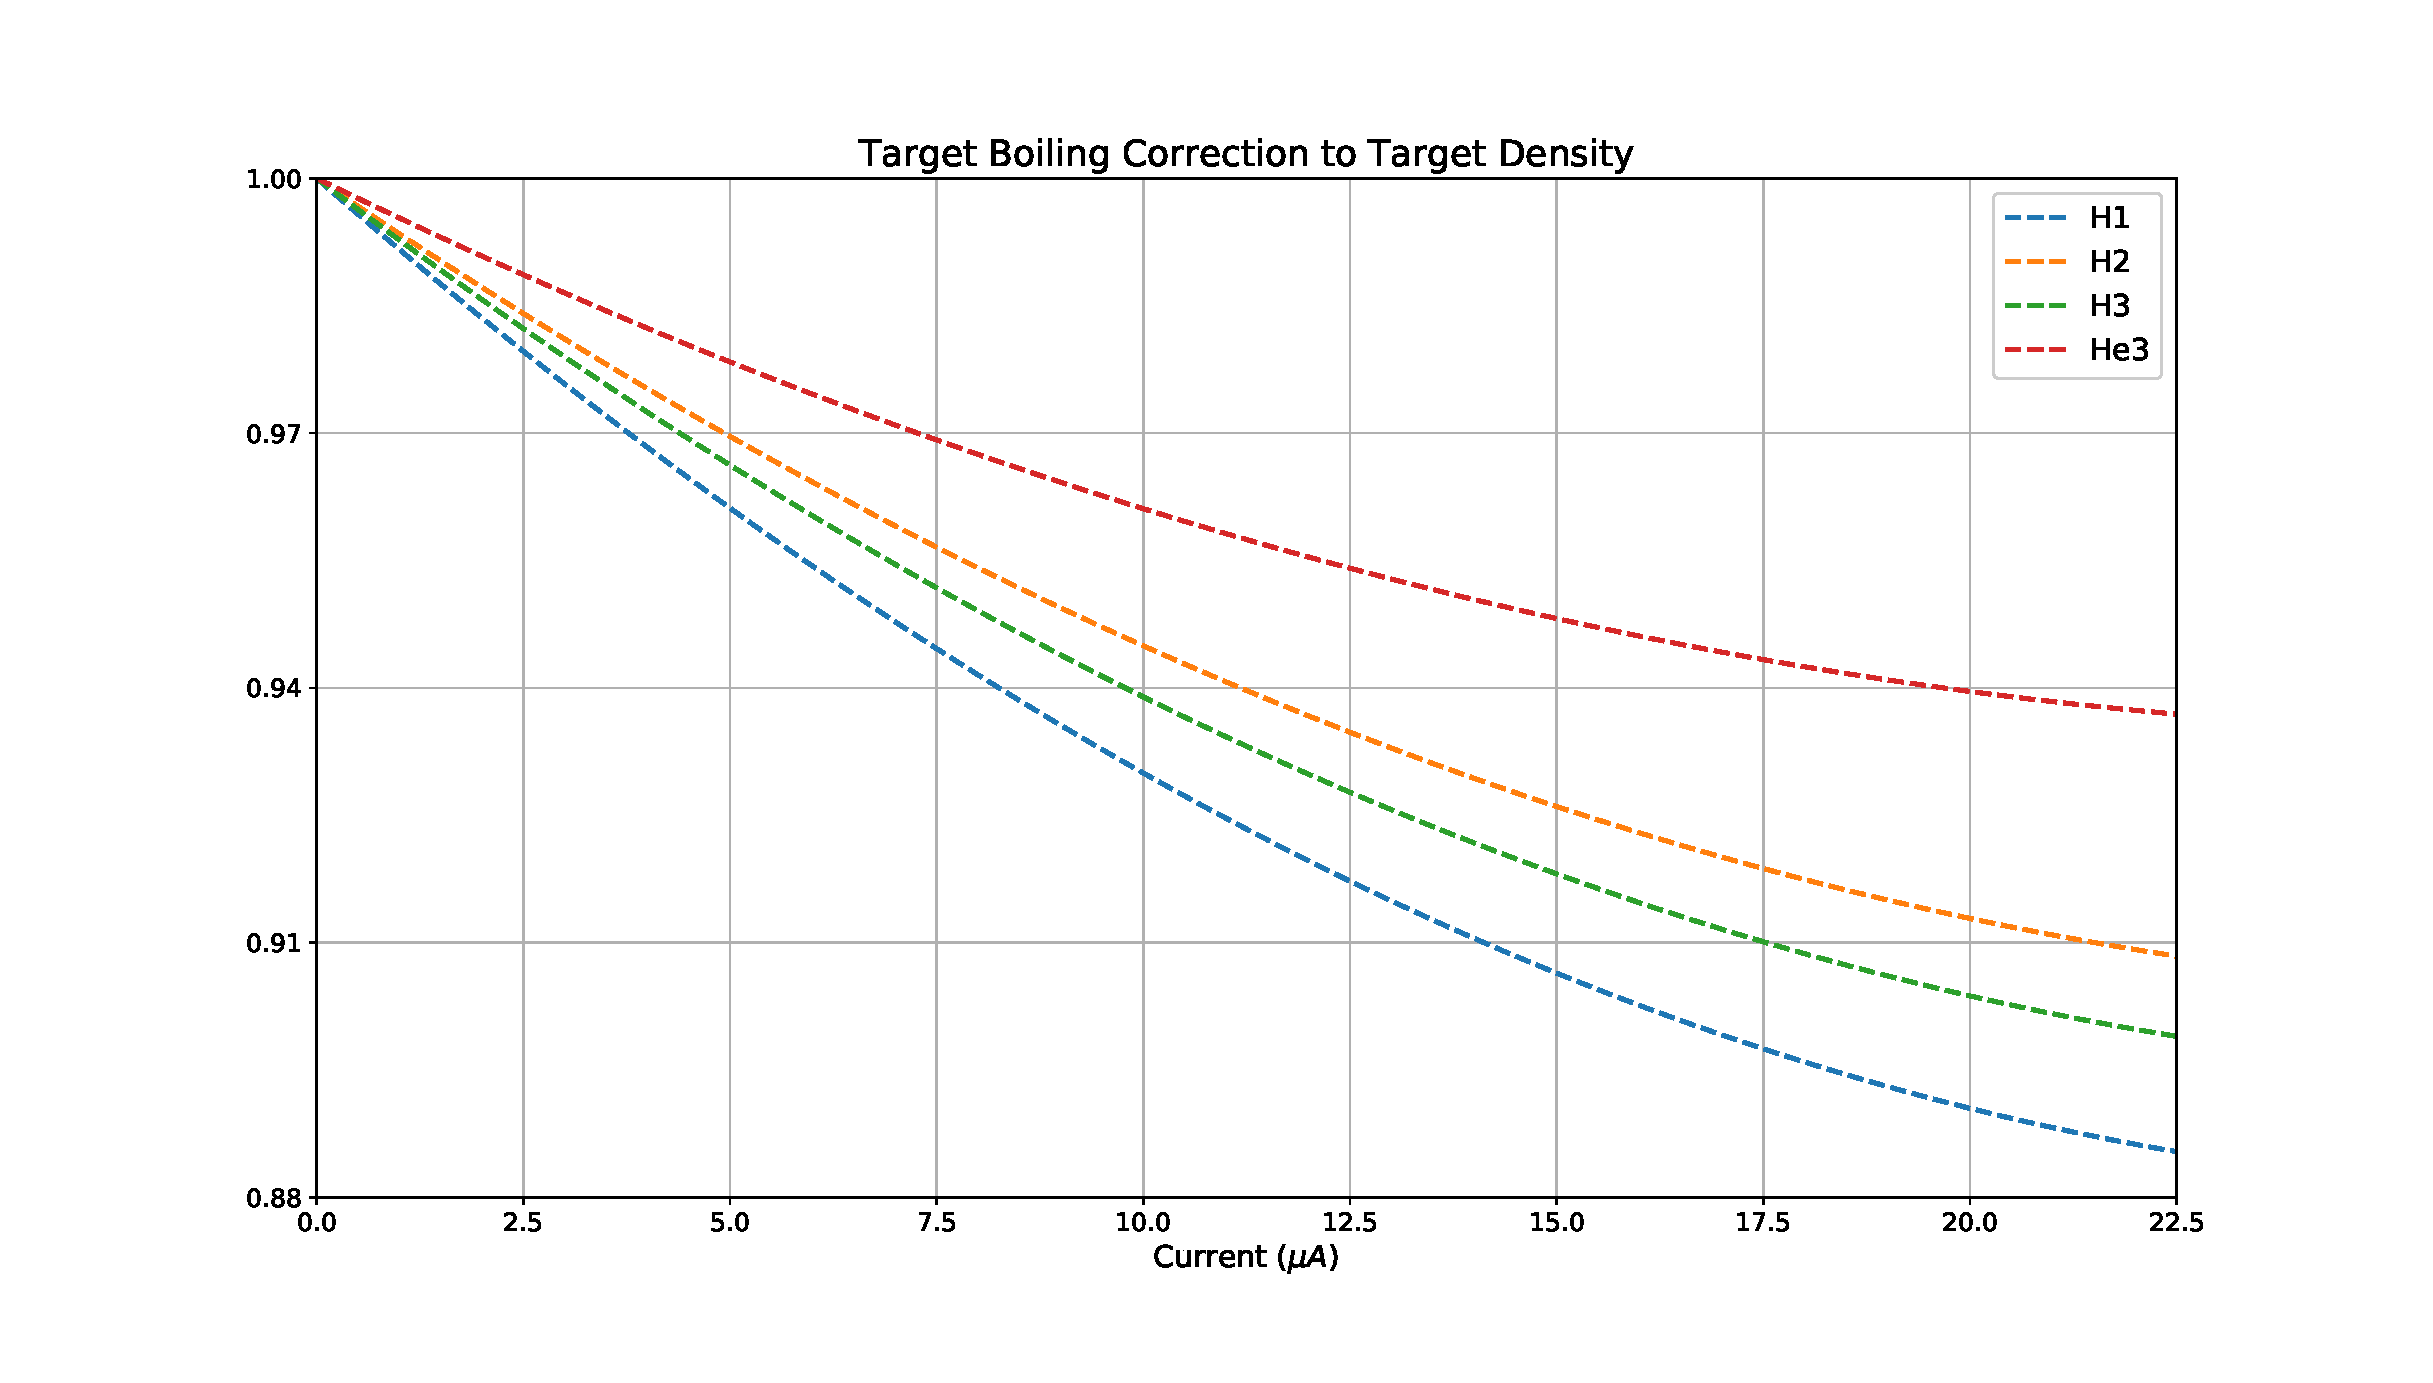
\includegraphics[width=\textwidth]{./analysis/fig/boil_cor.eps}
	\caption{Beam heating effects are manifested as a multiplicative correction to the target density}
	\label{fig:boilcor}
\end{figure}

%\begin{figure}
%	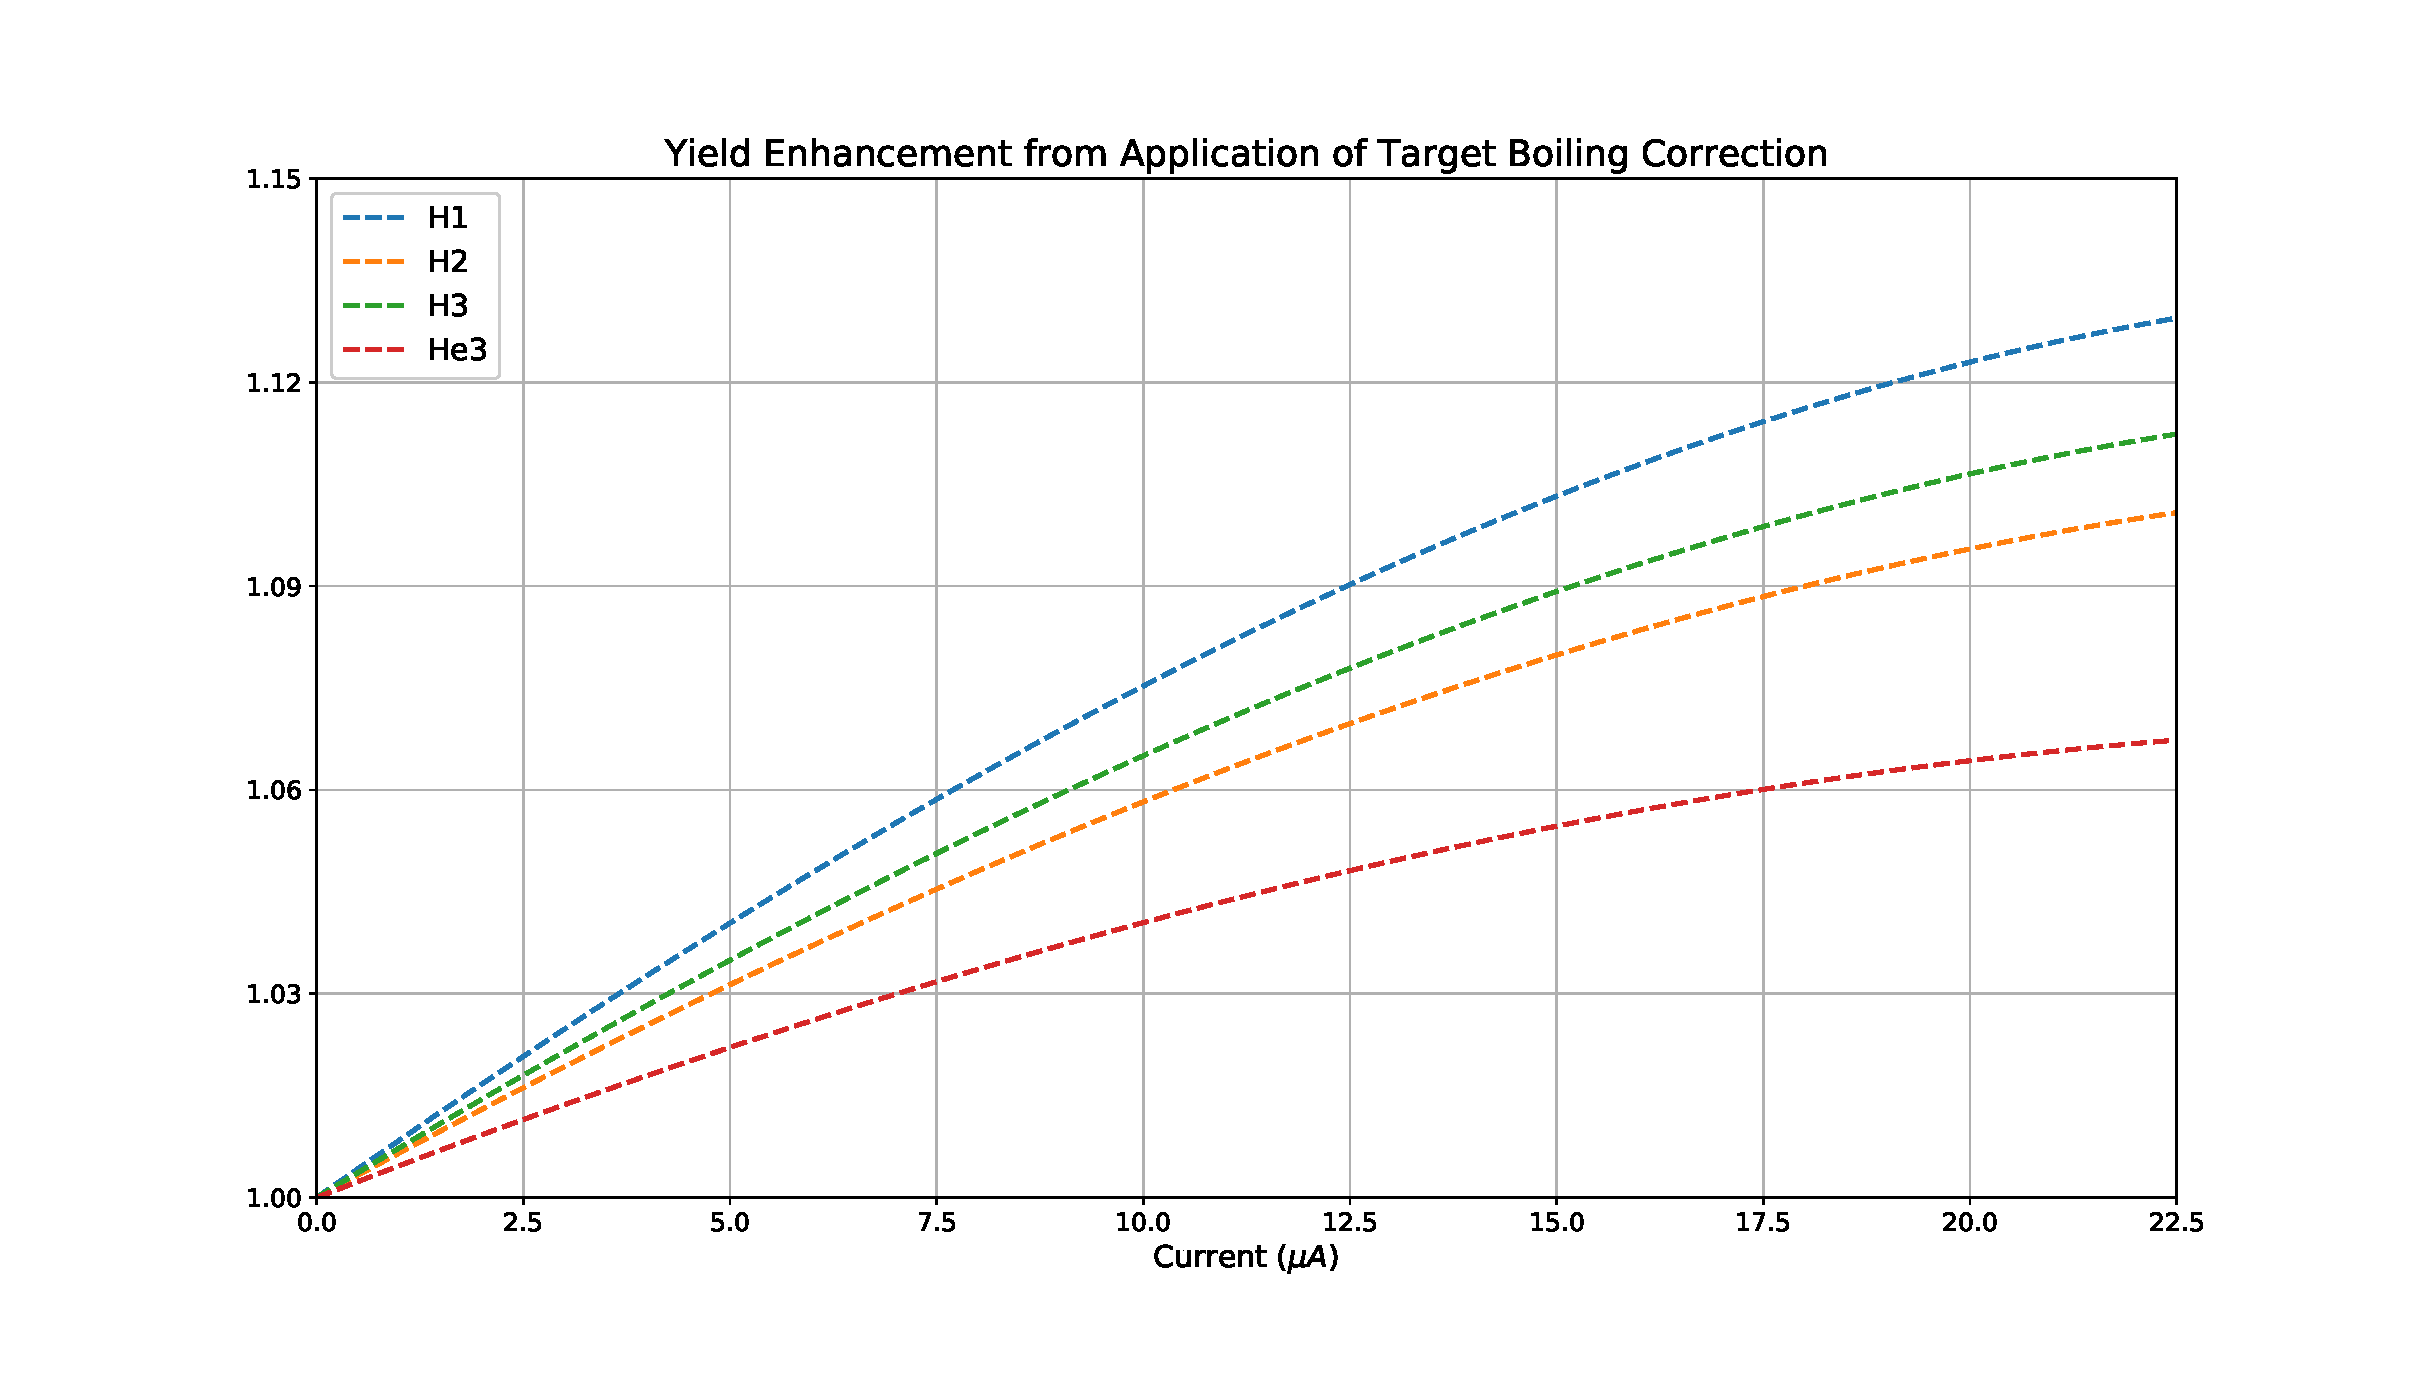
\includegraphics[width=\textwidth]{./analysis/fig/boil_yield_cor.eps}
%	\caption{Target density corrections cause a multiplicative enhancement to the yield}
%	\label{fig:boilyieldcor}
%\end{figure}

\subsection{Target Endcap Contamination}
\label{sec:ecc}

The gas targets used in this experiment are housed in aluminum cells as described in Section \ref{sec:gas_cell}. The thickness of the aluminum greatly exceeds the thickness of the gas and will contribute background that can survive the cuts placed on the data. By quantifying this contribution, the events that originate from the cell endcaps can be subtracted from the final results.

To determine this contribution, the empty cell is used. The empty cell, being an exact replica of the gas target cells with a vacuum inside, allows us to approximately isolate the contribution of the cell walls to the data. The empty cell and the target being studied are compared by calculating the yields on a kinematic-by-kinematic basis and normalizing them by charge and endcap thickness.

The normalization to the endcaps for each target must be done in two parts. This is because each endcap is not the same thickness. When calculating the yield for a target, it is assumed that any contamination upstream (downstream) of the center of the target must originate from the upstream (downstream) endcap. The two halves are then combined to arrive at the endcap thickness normalized yield. This yield calculation only has livetime corrections applied. All cuts are applied except for target length, which is adjusted to only include events upstream (downstream) of the center of the target.

The data for the target being studied and the normalized empty target are then binned in Bjorken $x$. Dividing the empty cell data by the gas target data then gives an approximation of the fractional contribution of the cell walls to the electron data. As this correction is applied to the final results, the contamination corrections for the targets are divided by each other to create the correction to the target ratios. These results are then fit with the functional form $1\pm e^{Ax+B}$. The choice of adding or subtracting the exponential is done by determining if the correction is greater or smaller than 1. The fit function and the covariance matrix of the fit are used to apply the correction to the final results as well as determine the uncertainty contribution of this correction.

\subsection{Charge Symmetric Background Subtraction}

As an inclusive scattering experiment, we are particularly susceptible to background from charge symmetric processes from the target. That is events which involved the production of both an electron and a positron, rather than the electron simply scattering. To study this, the polarity of the LHRS was reversed so that positively charge particles are directed into the detectors rather than negatively charged particles. With this setting, a number of runs were taken in kinematics 0 through 5. These runs were taken with all targets, just as the electron data was taken. This allows for a measurement of the positron yield which corresponds to a measure of the charge symmetric background.

This measurement allows us to determine the proportion of electrons that originated from pair production. Applying the same cuts and as the electron data allows us to determine the charge normalized positron yield. Unlike in the electron analysis, it was noted that there was significant pion contamination in the positron data. This pion contamination had to be subtracted in order to get an accurate calculation of the positron yield. This is achieved by fitting the main pion peak and the subtracting the tail of the fit which survives the cuts applied from the positron data.

The charge normalized positron yields over these kinematics are then combined (using the same methods as the electron yield) and binned in Bjorken $x$. This was then divided by the charge normalized electron yield. This is a fractional measure of the charge normalized background contamination. The ratio is then fit with an exponential of the form $e^{Ax + B}$, where $A$ and $B$ are the fit parameters. These fits are shown in in Figure \ref{fig:positrons}.

This correction is applied to the final yield ratio results. Both the numerator and denominator must have the charge symmetric background subtracted. Each target yield in the ratio is scaled by $1 - \left(\textrm{Charge Symmetric Background Fit}\right)$. For each bin, the fit is calculated at the bin center.

\begin{figure}
	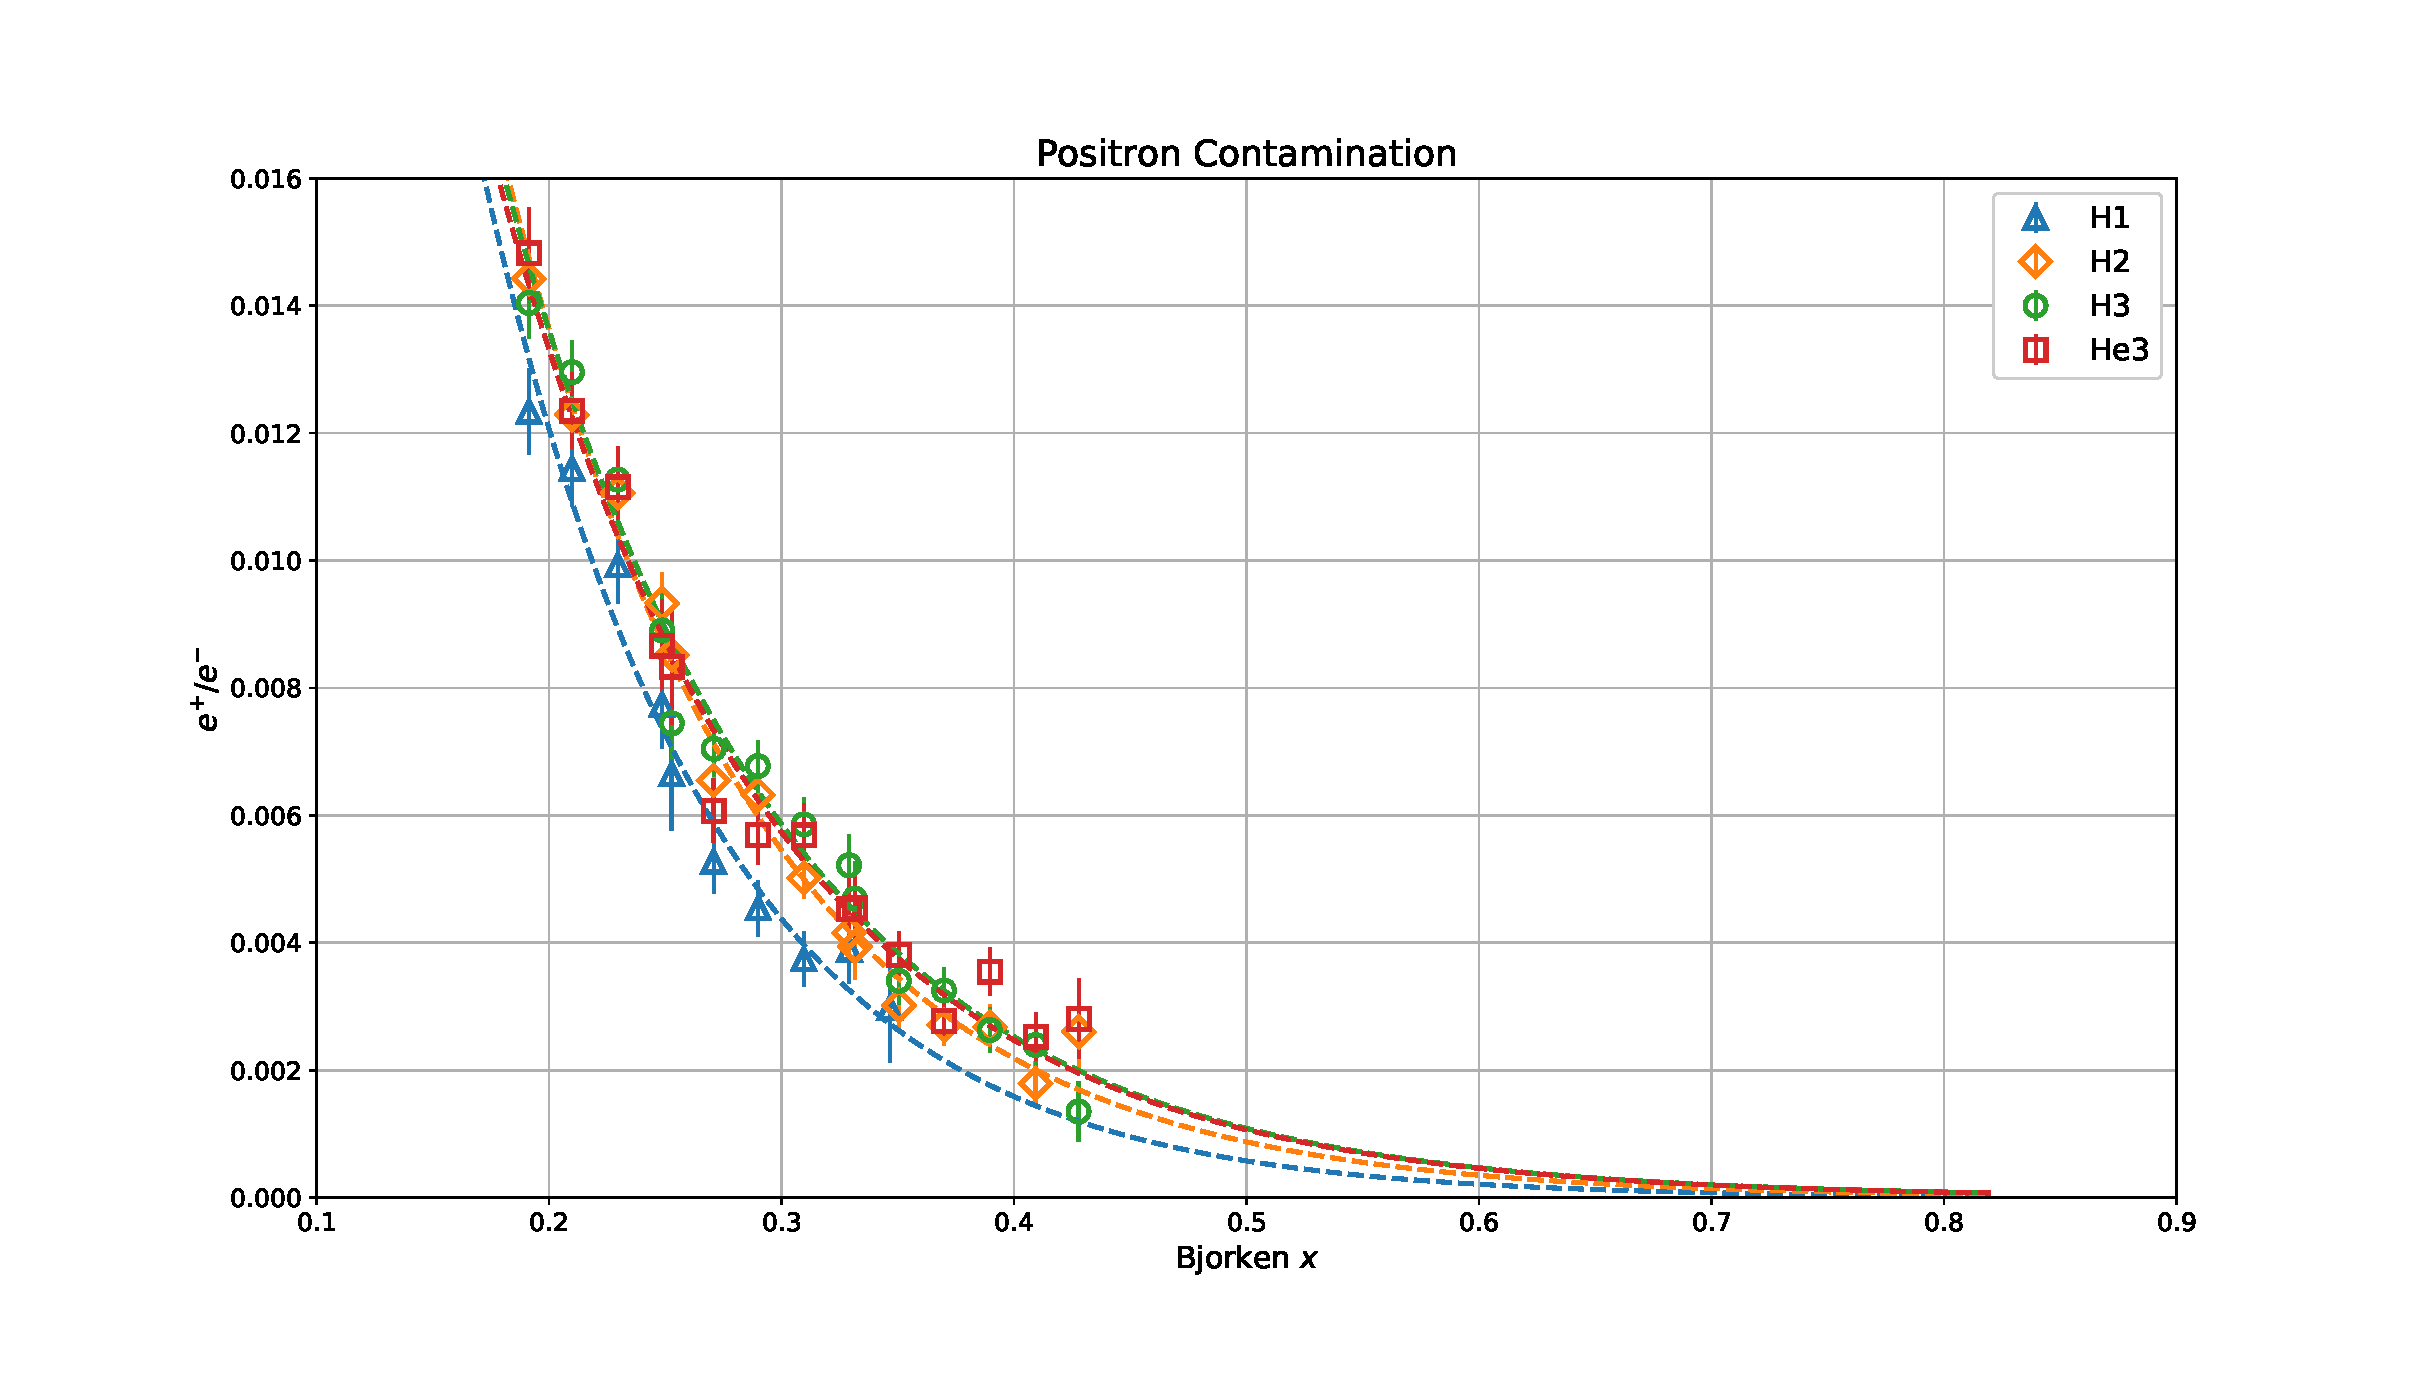
\includegraphics[width=\textwidth]{./analysis/fig/positrons.eps}
	\caption{Charge symmetric background correction}
	\label{fig:positrons}
\end{figure}

\subsection{Computer Deadtime Correction}

Our DAQ unable to continuously record data. While we can probabilistically determine the mean time spacing between events, in the real world events can deviate greatly from these means. Sometimes events will occur that are too close in time for our DAQ to record as the computer has not completed recording the previous event. Deadtime is a function of event rate; when events happen more rapidly, there is a higher chance that events will occur too closely in time to be recorded.

When deadtime is low and the number of recorded events is high, it is a reasonable assumption that the events recorded will accurately reflect the distribution of events in the ``zero-deadtime limit''. In this case correcting for the deadtime is simply done by scaling the number of events by the ``livetime'' of the experiment.

The computer livetime was measured using the Trigger Supervisor and scalers in each HRS. The trigger signals generated from detector signals are copied and sent to both the Trigger Supervisor and a scaler unit. The Trigger Supervisor is subject to the computer deadtime event loss discussed here. The scaler unit, on the other hand, simply increments a register when a trigger signal is received. The ratio of these the number of events recorded by these two systems gives a measure of the livetime of the measurement. The livetime is defined on a run-by-run basis as:

\begin{equation}
DT = \frac{\Sigma \mathrm{Triggers_{TS}}}{\Sigma \mathrm{Triggers_{Scaler}}}
\end{equation}

In an ideal world, the deadtime will be identical for all runs within a kinematic. However, the deadtime is measured on a run-by-run basis and is applied as such in order to account for any deviations from this assumption. The average deadtime for each target in each kinematic is plotted in Figure \ref{fig:deadtime}.

\begin{figure}
	\includegraphics[width=\textwidth]{./analysis/fig/deadtime.eps}
	\caption{Deadtime per kinematic}
	\label{fig:deadtime}
\end{figure}

\subsection{Radiative Corrections}

The Deep Inelastic Cross Sections being studied are the Born approximation of a single-photon exchange. The measurement however, contains contributions from higher order processes that will increase the measured cross section. Using a model, the contributions can be corrected for and removed from the measurement.

The experiment used a software package called $\texttt{T2\_EXTERNALS}$ that calculates both the Born cross section and the radiated cross section for a given target at a kinematic set $(E,E^{\prime} ,\theta )$.

\subsection{Isoscalar Corrections}

\subsection{Bin Centering Corrections}

The cross-section over the width of a bin is not constant. This means that the measurement does not correspond with the true cross section at the center of the bin. Using a model that matches the shape of our data well, the location of the measurement within the bin can be calculated. This is done by calculating the expectation value of the model within that bin and determining the $x$ value corresponding to this value. The expectation value is given by
\begin{equation}
	\langle f_{\rm measured}\rangle = \frac{1}{\Delta x}\int_{x_{\rm low}}^{x_{\rm high}} f\left( x \right) dx,
\end{equation}
where $f$ is a function representing the chosen model. In practice, the $x$ value does not need to be calculated if the data will be reported at the bin center. Rather, the correction is simply the ratio of the model at the bin center. This is written as
\begin{equation}
	\sigma_{\textrm{Bin Centered}} = \frac{f\left(x_{\textrm{Bin Center}}\right)}{\langle f_{\rm measured}\rangle} \sigma_{\rm measured}.
\end{equation}

This correction must be applied to both targets in the ratios. That is, the ratio must be multiplied by the correction to the numerator and divided by the correction to the denominator.\cite{wtsydp}

\subsection{Coulomb Corrections}

Corrections must be made for the effect of the charge of the target on the scattered electron. This interaction causes the $Q^2$ of the event to shift to an effective $Q^2$ value, $Q^2_{\rm eff}$. This conversion is done with the equation
\begin{equation}
	Q^2_{\rm eff} = Q^2 \left(1 + \frac{3Z\alpha\hbar c}{2RE}\right)^{2}.
\end{equation}
In this equation $R$ is the hard-sphere equivalent radius of the nucleus which is defined as $R=\left[\left(\nicefrac{5}{3}\right) \langle r^{2}\rangle\right]^{\nicefrac{1}{2}}$ where $\langle r^2\rangle$ is the root-mean-squared radius of the nucleus.\cite{coulomb}

Using $x=\frac{Q^2}{2M\nu}$, it is clear that a shift in $Q^2$ will result in a proportional shift in $x$. Using a model cross-section, the cross section is calculated at both the nominal $x$ and at $x_{\rm eff}$. As the results have been bin centered, this calculation uses a nominal $x$ at the center of the bin. This will lead to the correction
\begin{equation}
	\sigma_{\textrm{Coulomb Corrected}} = \sigma_{\rm data} \frac{\sigma_{\rm model}\left(x_{\rm eff}\right)}{\sigma_{\rm model}\left(x\right)}.
\end{equation}

This correction must be applied to both targets in the ratios that are calculated.
\subsection{Particle Identification}


\chapter{\bf{The EMC Effect}}             % Chapter  1
\setcounter{figure}{0}
\setcounter{table}{0}
\setcounter{equation}{0}
\section{Yield Calculation}

The MARATHON experiment measured cross section ratios. This method allows us to cancel many systematics that would otherwise plague a full cross section analysis. By taking data for each target at the same kinematics, acceptance effects are identical. This data taking technique means that with reasonable acceptance cuts, a ratio of target yields is wholly equivalent to the ratio of cross sections.

To calculate the yield we use a simple equation:

\begin{equation}
	\text{Yield} = \frac{\text{Counts}}{\text{Scattering Centers} \cdot \text{Livetime}} \cdot \text{Corrections}
\end{equation}

The yield is binned in Bjorken $x$. This chapter will explain the cuts and corrections that go into this calculation.

\section{Calibration}
\subsection{Raster Calibration}
\input{./chap3-analysis/raster_calib2.tex}


\section{Analysis}
\section{Corrections}

When analyzing the data, there are several corrections that need to be made. These are due to various physical or systematic effects that took place during the experiment. These effects have been studied in order to determine a ``correction factor'' that can be applied to the data.

\subsection{Target Boiling}
\label{sec:boiling}

When the beam is incident on the target, it deposits heat into the gas. This causes a density fluctuation of the gas referred to as ``target boiling''. The target does not actually boil, however that is the standard nomenclature for a density fluctuation in a gas target. When the density of the target changes, it changes the effective target thickness as seen by the beam. When the target thickness changes, there is a changed number of scattering centers which will lead to a change in the number of electrons recorded. Specifically, heating will decrease the target density which will decrease the number of scattered electrons.

The density changes are a function of the current on the target. Each run is taken at a single current so that the correction can be applied run by run. The correction is approximately linear for small deviations in current. A study of the effect during beam ramping found that the density settles very quickly. This means that so long as we cut events that occur with the beam off, it is unnecessary to take into account the beam ramping when correcting for this effect.

To determine the correction, a dedicated set of runs was taken with the Left HRS spectrometer at $16.8\degree$ and 3.1 GeV. At this kinematic, several data runs were recorded with varying current between them. Each of these runs were analyzed with the standard data cuts to determine the yield. This allows for the yield to be determined as a function of beam current.

Now that the yields have been determined as a function of beam current, they can be plotted and fit. The data is fit with a quadratic polynomial. This fit is constrained to require no correction (a correction factor of 1) at zero current. This is because the density must be the nominal fill density when there is no beam heating. During analysis the average current is calculated for a run (ignoring beam trips). The average current is then used to calculate the target density correction with the fit function. The correction is then applied on a run-by-run basis by multiplying the number of scattering centers by this correction factor (or equivalently dividing the yield by the correction factor). Figure \ref{fig:boilcor} shows the correction factors for each target.\cite{boiling}

\begin{figure}
	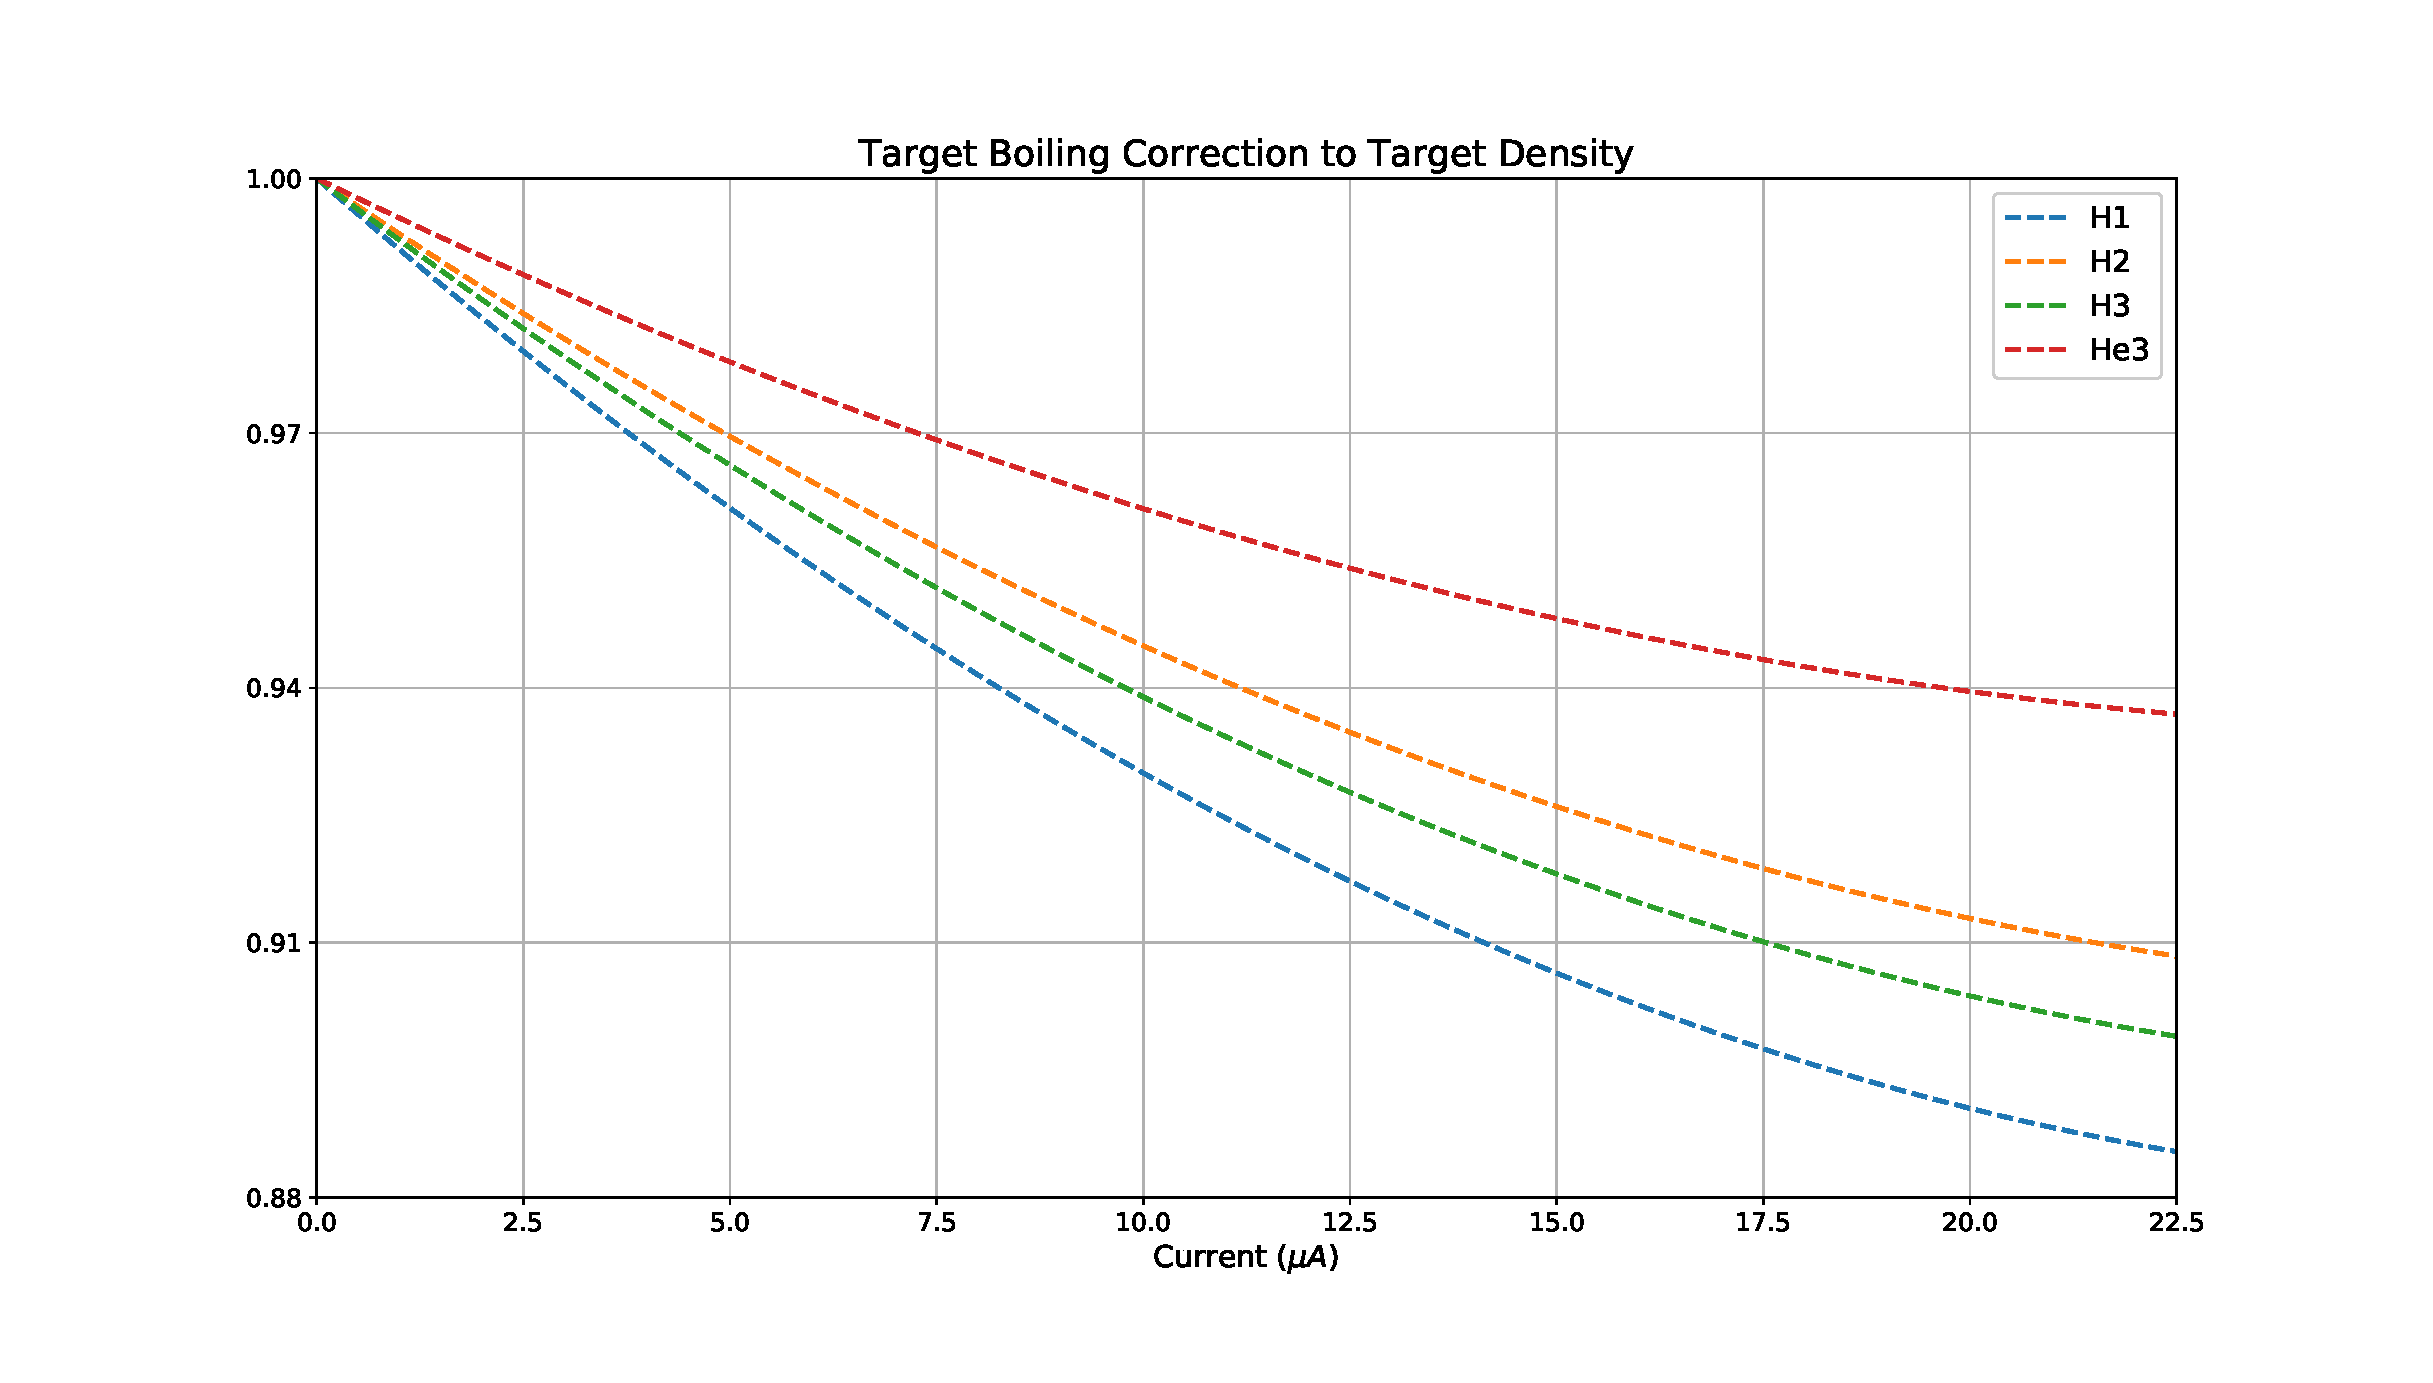
\includegraphics[width=\textwidth]{./analysis/fig/boil_cor.eps}
	\caption{Beam heating effects are manifested as a multiplicative correction to the target density}
	\label{fig:boilcor}
\end{figure}

%\begin{figure}
%	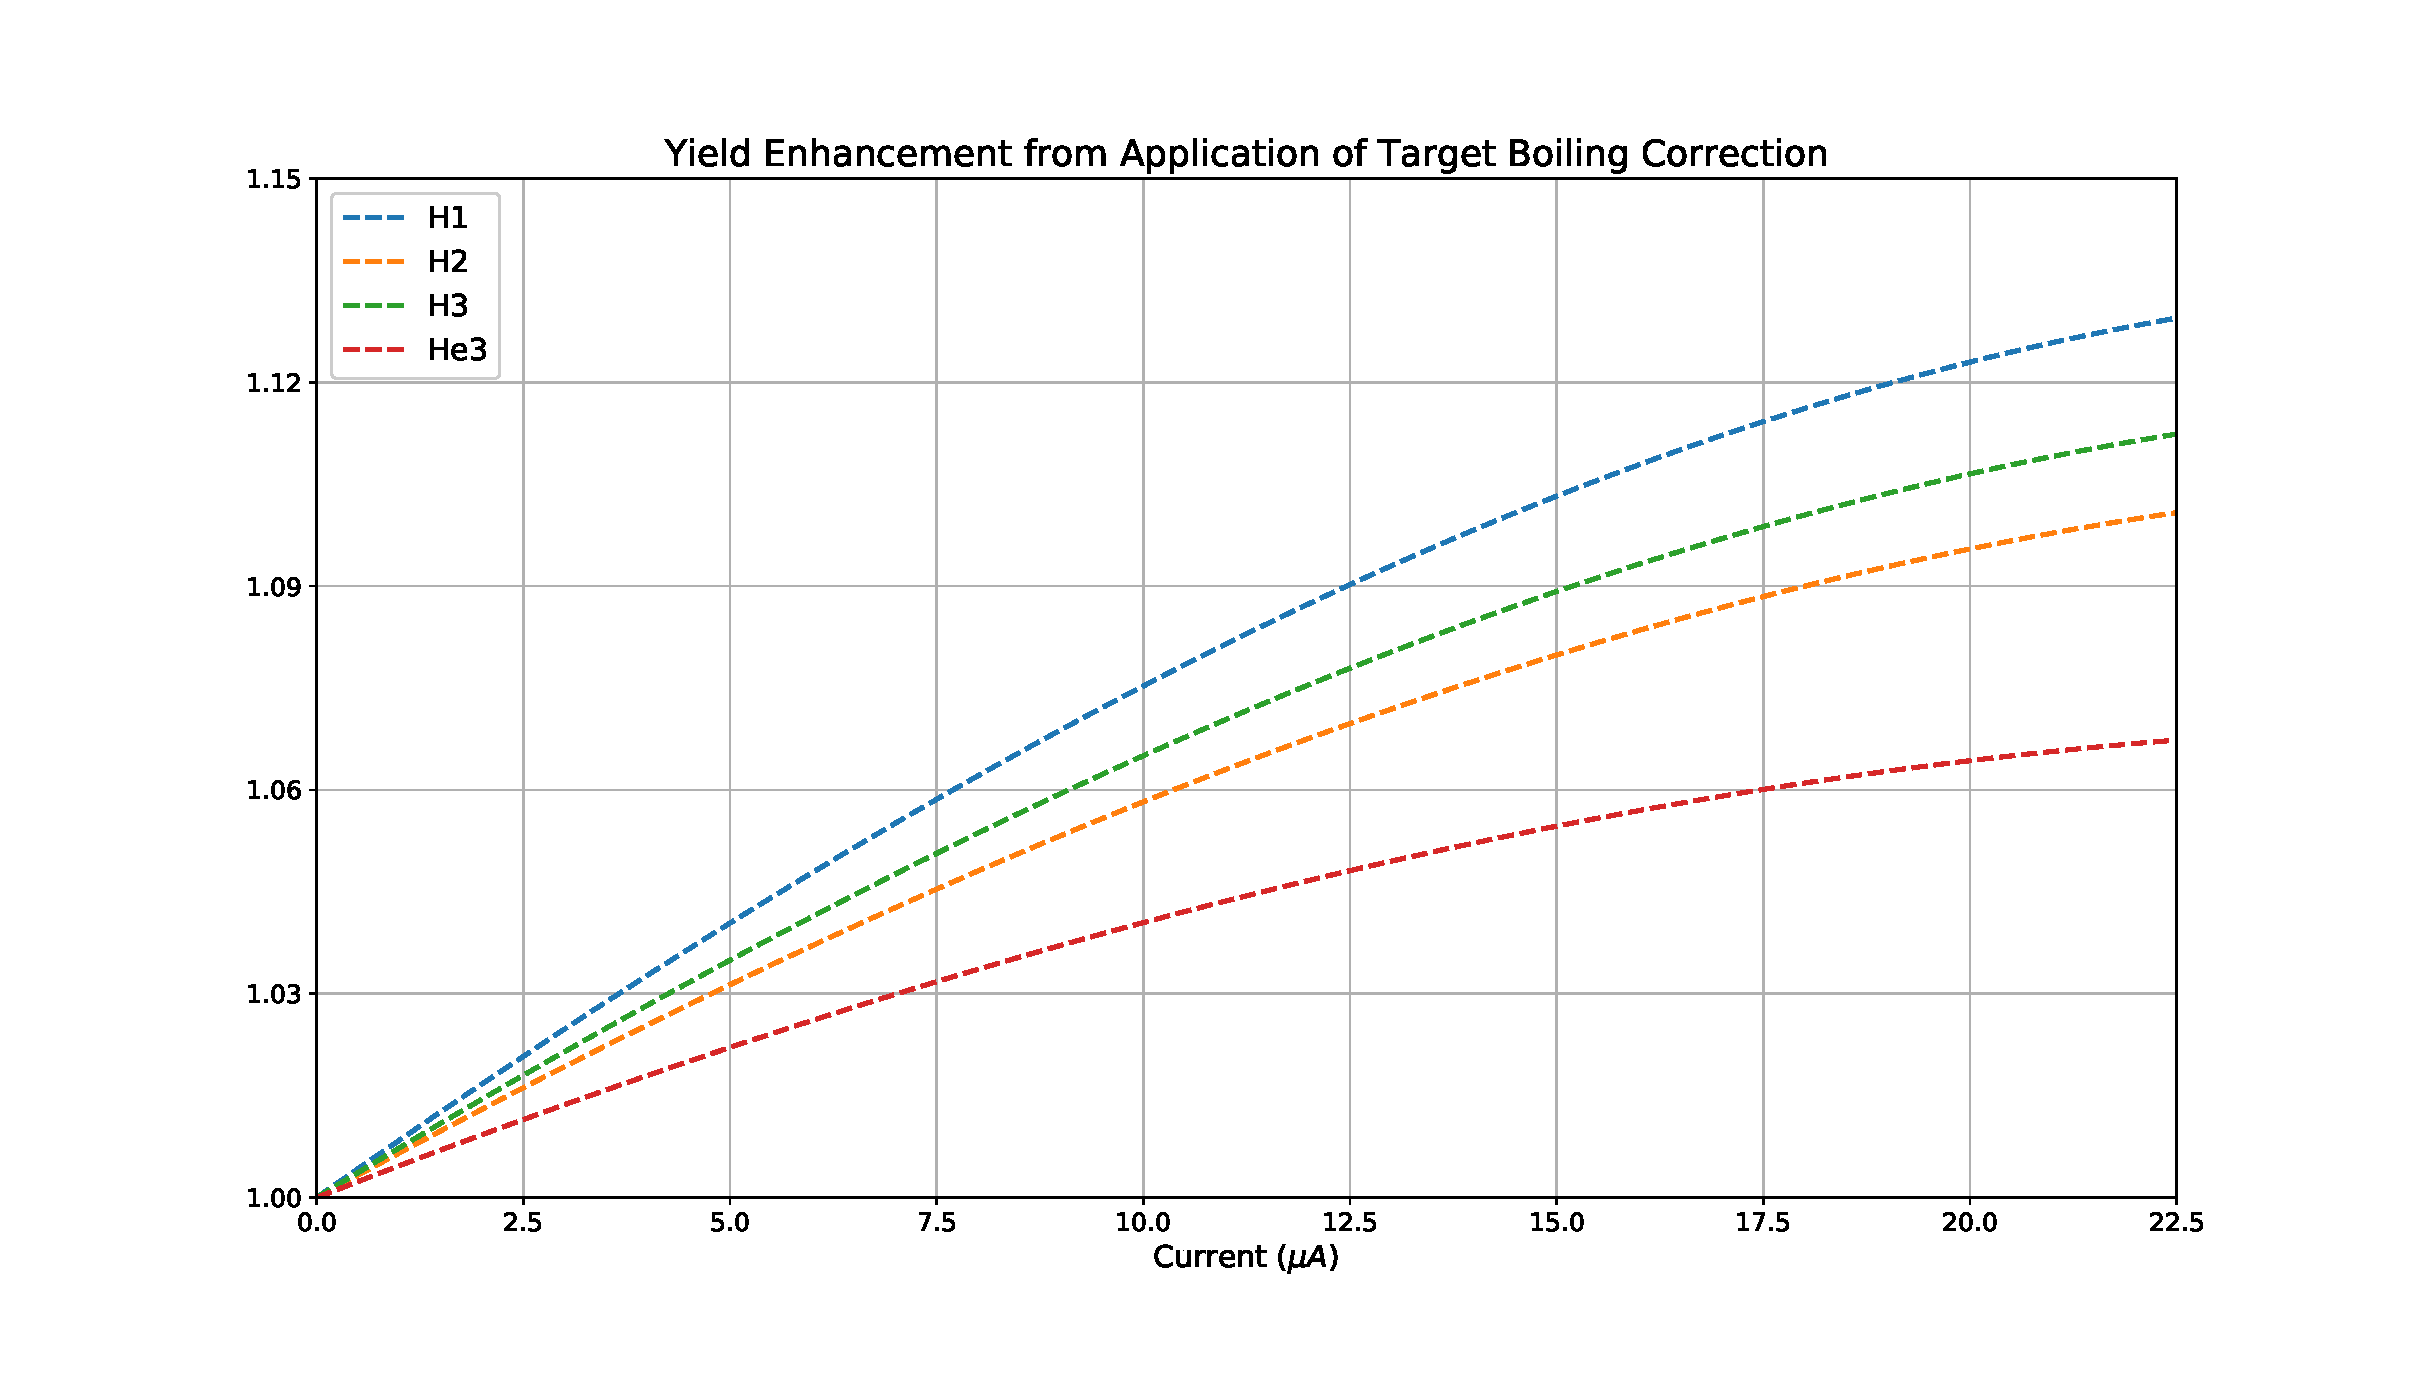
\includegraphics[width=\textwidth]{./analysis/fig/boil_yield_cor.eps}
%	\caption{Target density corrections cause a multiplicative enhancement to the yield}
%	\label{fig:boilyieldcor}
%\end{figure}

\subsection{Target Endcap Contamination}
\label{sec:ecc}

The gas targets used in this experiment are housed in aluminum cells as described in Section \ref{sec:gas_cell}. The thickness of the aluminum greatly exceeds the thickness of the gas and will contribute background that can survive the cuts placed on the data. By quantifying this contribution, the events that originate from the cell endcaps can be subtracted from the final results.

To determine this contribution, the empty cell is used. The empty cell, being an exact replica of the gas target cells with a vacuum inside, allows us to approximately isolate the contribution of the cell walls to the data. The empty cell and the target being studied are compared by calculating the yields on a kinematic-by-kinematic basis and normalizing them by charge and endcap thickness.

The normalization to the endcaps for each target must be done in two parts. This is because each endcap is not the same thickness. When calculating the yield for a target, it is assumed that any contamination upstream (downstream) of the center of the target must originate from the upstream (downstream) endcap. The two halves are then combined to arrive at the endcap thickness normalized yield. This yield calculation only has livetime corrections applied. All cuts are applied except for target length, which is adjusted to only include events upstream (downstream) of the center of the target.

The data for the target being studied and the normalized empty target are then binned in Bjorken $x$. Dividing the empty cell data by the gas target data then gives an approximation of the fractional contribution of the cell walls to the electron data. As this correction is applied to the final results, the contamination corrections for the targets are divided by each other to create the correction to the target ratios. These results are then fit with the functional form $1\pm e^{Ax+B}$. The choice of adding or subtracting the exponential is done by determining if the correction is greater or smaller than 1. The fit function and the covariance matrix of the fit are used to apply the correction to the final results as well as determine the uncertainty contribution of this correction.

\subsection{Charge Symmetric Background Subtraction}

As an inclusive scattering experiment, we are particularly susceptible to background from charge symmetric processes from the target. That is events which involved the production of both an electron and a positron, rather than the electron simply scattering. To study this, the polarity of the LHRS was reversed so that positively charge particles are directed into the detectors rather than negatively charged particles. With this setting, a number of runs were taken in kinematics 0 through 5. These runs were taken with all targets, just as the electron data was taken. This allows for a measurement of the positron yield which corresponds to a measure of the charge symmetric background.

This measurement allows us to determine the proportion of electrons that originated from pair production. Applying the same cuts and as the electron data allows us to determine the charge normalized positron yield. Unlike in the electron analysis, it was noted that there was significant pion contamination in the positron data. This pion contamination had to be subtracted in order to get an accurate calculation of the positron yield. This is achieved by fitting the main pion peak and the subtracting the tail of the fit which survives the cuts applied from the positron data.

The charge normalized positron yields over these kinematics are then combined (using the same methods as the electron yield) and binned in Bjorken $x$. This was then divided by the charge normalized electron yield. This is a fractional measure of the charge normalized background contamination. The ratio is then fit with an exponential of the form $e^{Ax + B}$, where $A$ and $B$ are the fit parameters. These fits are shown in in Figure \ref{fig:positrons}.

This correction is applied to the final yield ratio results. Both the numerator and denominator must have the charge symmetric background subtracted. Each target yield in the ratio is scaled by $1 - \left(\textrm{Charge Symmetric Background Fit}\right)$. For each bin, the fit is calculated at the bin center.

\begin{figure}
	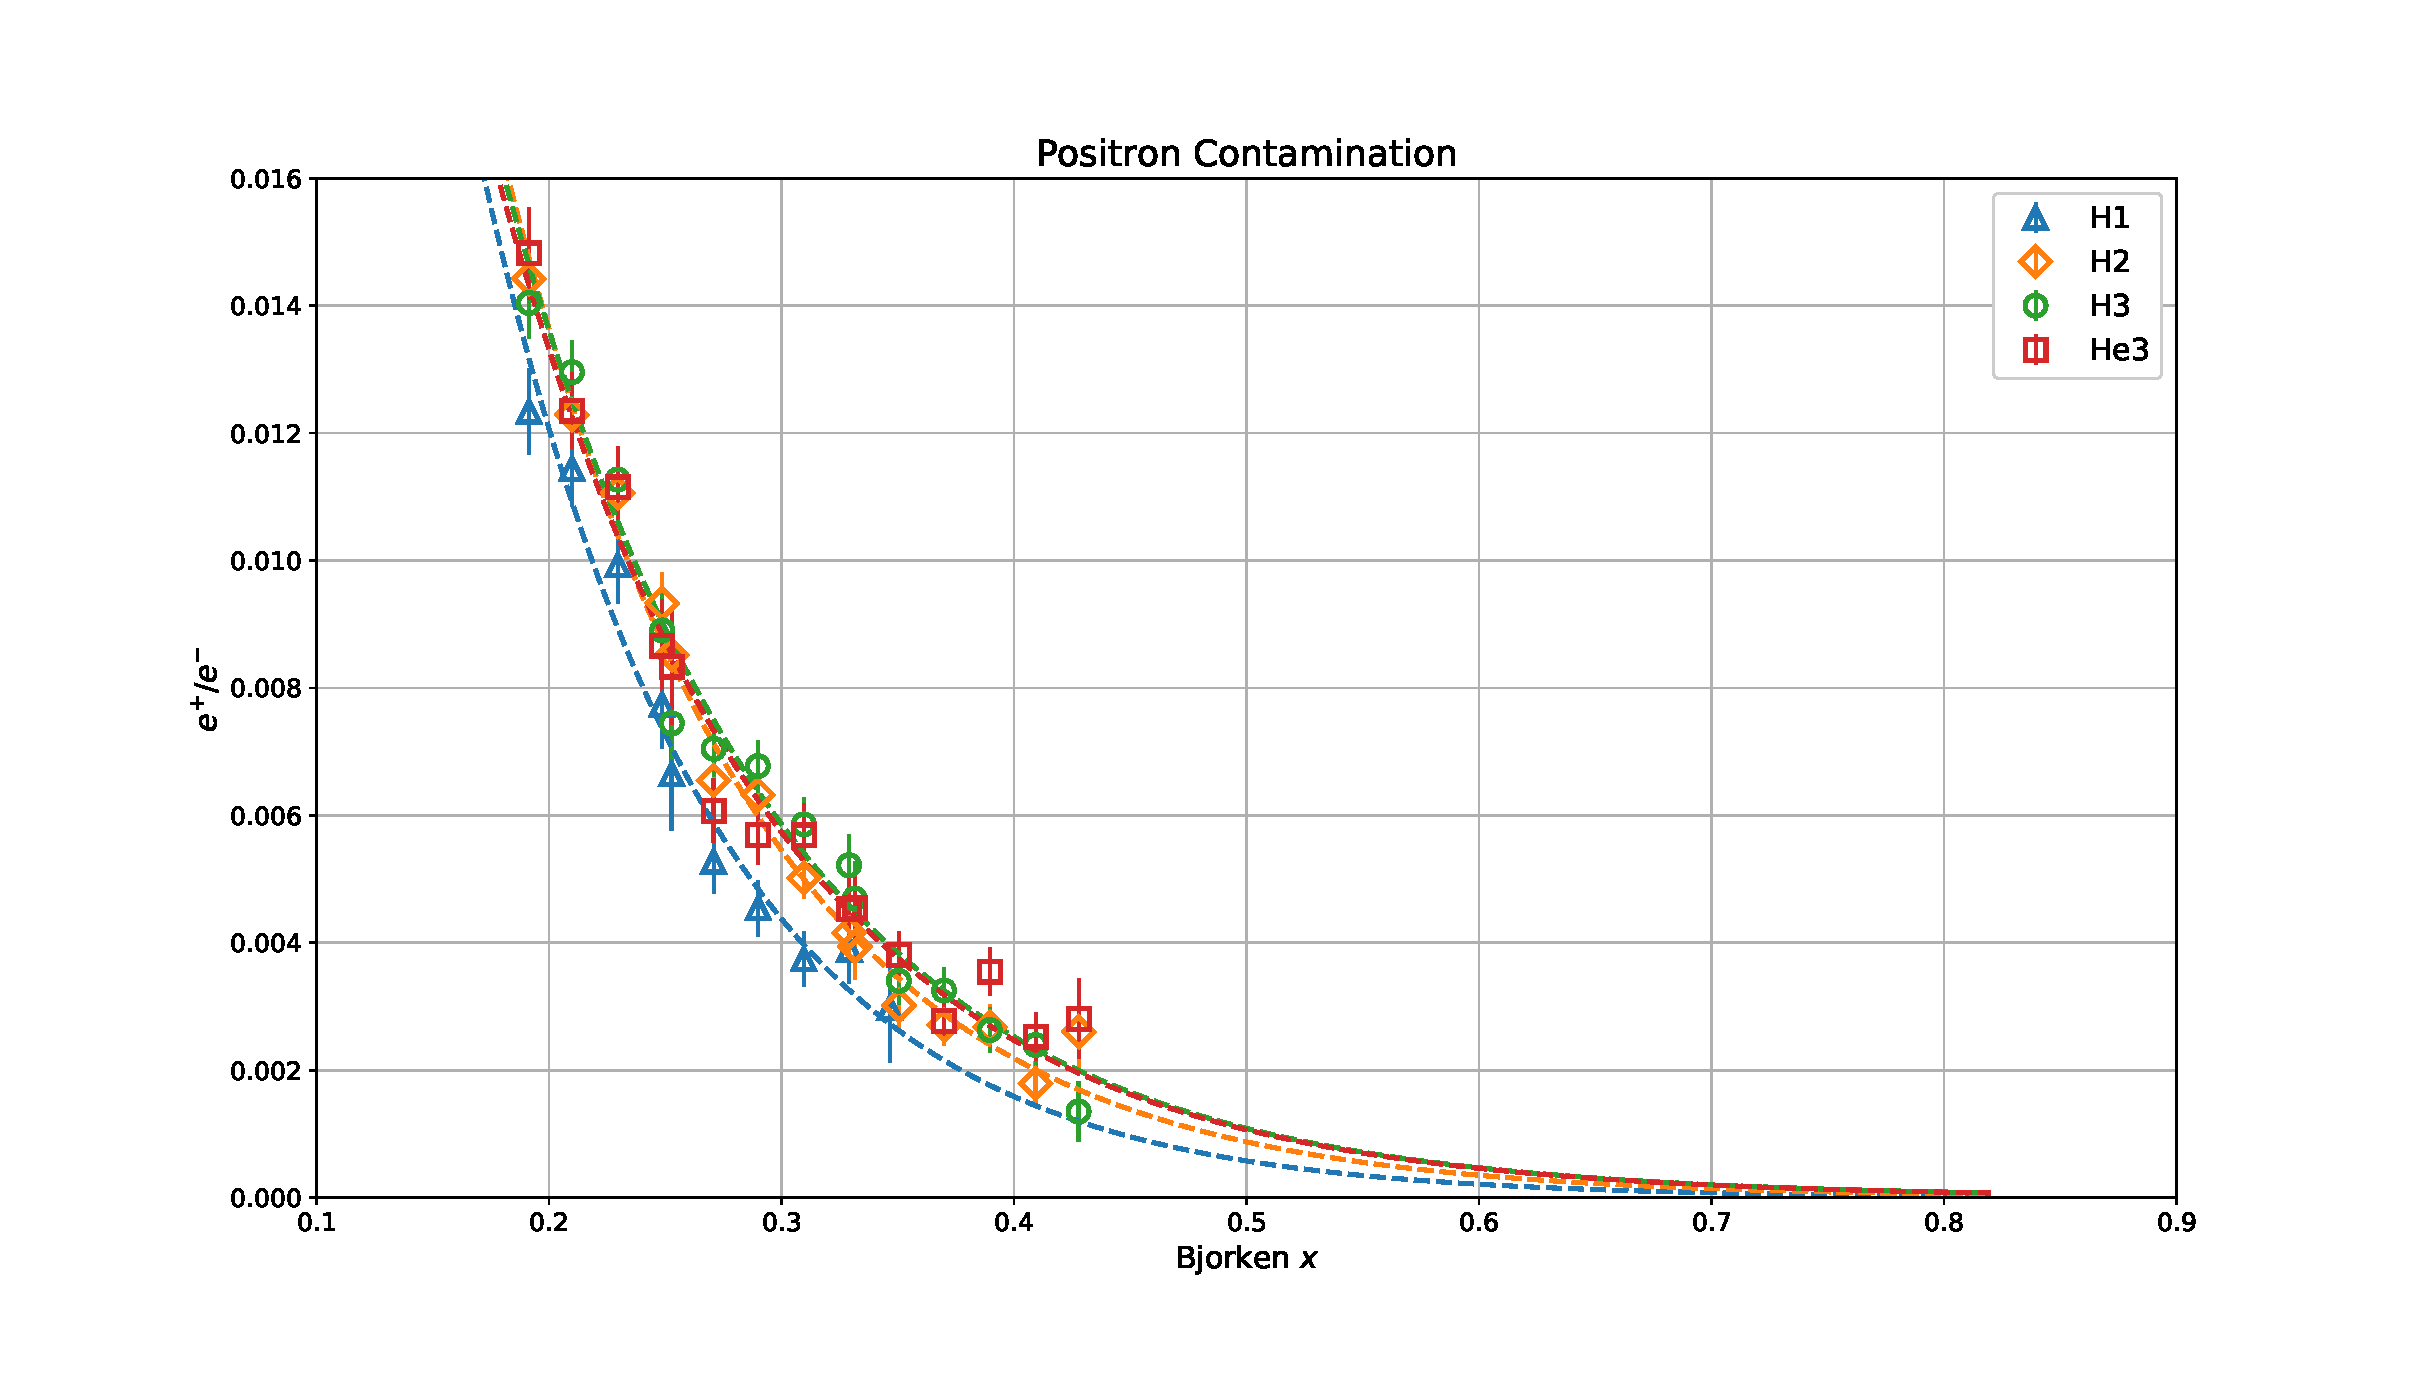
\includegraphics[width=\textwidth]{./analysis/fig/positrons.eps}
	\caption{Charge symmetric background correction}
	\label{fig:positrons}
\end{figure}

\subsection{Computer Deadtime Correction}

Our DAQ unable to continuously record data. While we can probabilistically determine the mean time spacing between events, in the real world events can deviate greatly from these means. Sometimes events will occur that are too close in time for our DAQ to record as the computer has not completed recording the previous event. Deadtime is a function of event rate; when events happen more rapidly, there is a higher chance that events will occur too closely in time to be recorded.

When deadtime is low and the number of recorded events is high, it is a reasonable assumption that the events recorded will accurately reflect the distribution of events in the ``zero-deadtime limit''. In this case correcting for the deadtime is simply done by scaling the number of events by the ``livetime'' of the experiment.

The computer livetime was measured using the Trigger Supervisor and scalers in each HRS. The trigger signals generated from detector signals are copied and sent to both the Trigger Supervisor and a scaler unit. The Trigger Supervisor is subject to the computer deadtime event loss discussed here. The scaler unit, on the other hand, simply increments a register when a trigger signal is received. The ratio of these the number of events recorded by these two systems gives a measure of the livetime of the measurement. The livetime is defined on a run-by-run basis as:

\begin{equation}
DT = \frac{\Sigma \mathrm{Triggers_{TS}}}{\Sigma \mathrm{Triggers_{Scaler}}}
\end{equation}

In an ideal world, the deadtime will be identical for all runs within a kinematic. However, the deadtime is measured on a run-by-run basis and is applied as such in order to account for any deviations from this assumption. The average deadtime for each target in each kinematic is plotted in Figure \ref{fig:deadtime}.

\begin{figure}
	\includegraphics[width=\textwidth]{./analysis/fig/deadtime.eps}
	\caption{Deadtime per kinematic}
	\label{fig:deadtime}
\end{figure}

\subsection{Radiative Corrections}

The Deep Inelastic Cross Sections being studied are the Born approximation of a single-photon exchange. The measurement however, contains contributions from higher order processes that will increase the measured cross section. Using a model, the contributions can be corrected for and removed from the measurement.

The experiment used a software package called $\texttt{T2\_EXTERNALS}$ that calculates both the Born cross section and the radiated cross section for a given target at a kinematic set $(E,E^{\prime} ,\theta )$.

\subsection{Isoscalar Corrections}

\subsection{Bin Centering Corrections}

The cross-section over the width of a bin is not constant. This means that the measurement does not correspond with the true cross section at the center of the bin. Using a model that matches the shape of our data well, the location of the measurement within the bin can be calculated. This is done by calculating the expectation value of the model within that bin and determining the $x$ value corresponding to this value. The expectation value is given by
\begin{equation}
	\langle f_{\rm measured}\rangle = \frac{1}{\Delta x}\int_{x_{\rm low}}^{x_{\rm high}} f\left( x \right) dx,
\end{equation}
where $f$ is a function representing the chosen model. In practice, the $x$ value does not need to be calculated if the data will be reported at the bin center. Rather, the correction is simply the ratio of the model at the bin center. This is written as
\begin{equation}
	\sigma_{\textrm{Bin Centered}} = \frac{f\left(x_{\textrm{Bin Center}}\right)}{\langle f_{\rm measured}\rangle} \sigma_{\rm measured}.
\end{equation}

This correction must be applied to both targets in the ratios. That is, the ratio must be multiplied by the correction to the numerator and divided by the correction to the denominator.\cite{wtsydp}

\subsection{Coulomb Corrections}

Corrections must be made for the effect of the charge of the target on the scattered electron. This interaction causes the $Q^2$ of the event to shift to an effective $Q^2$ value, $Q^2_{\rm eff}$. This conversion is done with the equation
\begin{equation}
	Q^2_{\rm eff} = Q^2 \left(1 + \frac{3Z\alpha\hbar c}{2RE}\right)^{2}.
\end{equation}
In this equation $R$ is the hard-sphere equivalent radius of the nucleus which is defined as $R=\left[\left(\nicefrac{5}{3}\right) \langle r^{2}\rangle\right]^{\nicefrac{1}{2}}$ where $\langle r^2\rangle$ is the root-mean-squared radius of the nucleus.\cite{coulomb}

Using $x=\frac{Q^2}{2M\nu}$, it is clear that a shift in $Q^2$ will result in a proportional shift in $x$. Using a model cross-section, the cross section is calculated at both the nominal $x$ and at $x_{\rm eff}$. As the results have been bin centered, this calculation uses a nominal $x$ at the center of the bin. This will lead to the correction
\begin{equation}
	\sigma_{\textrm{Coulomb Corrected}} = \sigma_{\rm data} \frac{\sigma_{\rm model}\left(x_{\rm eff}\right)}{\sigma_{\rm model}\left(x\right)}.
\end{equation}

This correction must be applied to both targets in the ratios that are calculated.
\subsection{Particle Identification}


\chapter{\bf{The Experiment}}    % Chapter  2
\setcounter{figure}{0}
\setcounter{table}{0}
\setcounter{equation}{0}
\section{The Measurement}
\subsection{What are we measuring}
\subsection{How are we measuring it}
\subsection{Run Plan}

\section{The Apparatus}
\subsection{Hall A HRS Spectrometers}
\subsection{CEBAF Accelerator}

% \chapter{\bf{Chapter 2 Title}    % Chapter  2
%Introductory paragraph of Chapter 2.......
%
%\section{First section Title}
%
%First section text......
%
%
%
%\subsection{First Subsection Title}
%
%
%The cross section for elastic electron scattering from the spin one-half
%$^3$H  nucleus is given, in the one-photon exchange approximation, by:
%\beqn
%{  {d\sigma} \over {d\Omega} } (E,\Theta)  =
%{  {(Z\alpha)^2 E^\prime} \over {4 E^3  \sin^4 \left( {\Theta \over 2} \right)}  }
%\left[ A(Q^2) \cos^2 \left( {\Theta \over 2} \right) +
%B(Q^2) \sin^2 \left( {\Theta \over 2} \right) \right],
%\label{morefequ}
%\eeqn
%where $Z$ is the nuclear charge, $\alpha$ is the fine-structure constant,
%$E$ and $E'$ are the incident and scattered electron energies,
%$\Theta$ is the electron scattering angle, $Q^2 = 4 E E' \sin^2 (\Theta/2)$ is
%minus the squared four-momentum transfer,
%and $A(Q^2)$ and $B(Q^2)$ are the $^3$H elastic structure functions, given in
%terms of the charge and magnetic form factors as:
%\beqn
%{   A(Q^2) = {   { F^2_C(Q^2) +
%(1+\kappa)^2 \tau F^2_M(Q^2) } \over {1 + \tau} }    },
%\label{more1}
%\eeqn
%\beqn
%{ B(Q^2) =  2 \tau (1+\kappa)^2 F^2_M(Q^2) },
%\label{more2}
%\eeqn
%where
%$\tau=Q^2/4M^2$ with $M$ being the mass of the target nucleus, and
%$\kappa$ is the anomalous magnetic moment of the nucleus.
%
%Here is a reference ~\cite{mara} which needs to be defined in the bibliography.tex file first.
%
%
%Here comes a Figure....
%
% \begin{figure}[!htbp]
%  \begin{center}
%    \includegraphics[angle=90, scale=0.65]{./chap2-exp/fig/tritium_past.eps}
%  \end{center}
%  \caption[Tritium Magnetic Form Factor Past Data]{
%    \footnotesize Tritium Mag. Form Factor past data.
%  }
%  \label{fig:TritiumM}
%\end{figure}
%
%Use the label name to refer to  Figure  ~\ref{fig:TritiumM}.
%
%
%\subsection{Second Subsection  Title}
%
%Subsection text..........
%
%
%
%\subsubsection{First Subsubsection}
%
%This is a subsubsection.
%
%
%
%\subsubsection{Second Subsubsection}
%
%This another  subsubsection.

\setcounter{figure}{0}
\setcounter{table}{0}
\setcounter{equation}{0}
\subsection{Raster}
%Put this in order they appear in beamline?
\section{Beamline Components}

The Hall A Beamline has several measurement devices that allow the experimenter to fully understand the beam that is being delivered to the hall. For positioning, there are the Beam Position Monitors and the Harp. For beamspot sizing, there is the raster. For current and charge measurements, there are the Beam Current Monitors.

\subsection{Beam Position Monitors}

The Beam Position Monitors (BPMs) are a pair of measurement devices that consist of four sensing wires. By calibrating the signal received from each wire, the experimenter can reconstruct the position of the beam as it passed the BPM. Using both BPMs in conjunction allows the experimenter to determine the beam trajectory and where the electrons are incident on the target.

The BPMs are calibrated using a Harp fork. The Harp consists of three wires that are introduced sequentially into the path of the beam using a stepper motor. When the beam is incident on a wire, a charge is induced. By determining when each wire is struck by the beam, the experimenter can very accurately determine the position of the beam. This is an invasive measurement.

\subsection{Raster}
\begin{figure}
	\includegraphics[width=\linewidth]{./chap2-exp/fig/raster_pic.jpg}
	\caption{The Hall A raster consists of four dipole magnets on the beamline}
	\label{fig:raster}
\end{figure}

The raster is a beamline apparatus in Hall A for spreading the beam onto the target, rather than being at a single point. This is done to prevent localized heating of the target. The raster consists of four dipole magnets, two for steering in the x-direction and two for steering in the y-direction.

Each raster magnet is powered by a triangle wave of different frequencies to minimize harmonics. The horizontal rasters are set to 24.5 kHz and the vertical rasters are set to 25 kHz. When running properly, the x-direction magnets will be synced and the y-direction magnets will be synced. This syncing ensures that the magnets are always working together to create the desired beam spread.

\begin{figure}
	\includegraphics[width=\linewidth]{./chap2-exp/fig/raster_sync.png}
	\caption{The X and Y raster pairs are each synced to produce the maximum kick. The X and Y directions are uncorrelated so that the beam travels uniformly over the target.}
	\label{fig:raster}
\end{figure}

\subsection{Beam Current Monitors}


\chapter{\bf{Analysis}}    % Chapter  3
\setcounter{figure}{0}
\setcounter{table}{0}
\setcounter{equation}{0}
\section{Yield Calculation}

The MARATHON experiment measured cross section ratios. This method allows us to cancel many systematics that would otherwise plague a full cross section analysis. By taking data for each target at the same kinematics, acceptance effects are identical. This data taking technique means that with reasonable acceptance cuts, a ratio of target yields is wholly equivalent to the ratio of cross sections.

To calculate the yield we use a simple equation:

\begin{equation}
	\text{Yield} = \frac{\text{Counts}}{\text{Scattering Centers} \cdot \text{Livetime}} \cdot \text{Corrections}
\end{equation}

The yield is binned in Bjorken $x$. This chapter will explain the cuts and corrections that go into this calculation.

\section{Calibration}
\subsection{Raster Calibration}
\input{./chap3-analysis/raster_calib2.tex}


\section{Analysis}
\section{Corrections}

When analyzing the data, there are several corrections that need to be made. These are due to various physical or systematic effects that took place during the experiment. These effects have been studied in order to determine a ``correction factor'' that can be applied to the data.

\subsection{Target Boiling}
\label{sec:boiling}

When the beam is incident on the target, it deposits heat into the gas. This causes a density fluctuation of the gas referred to as ``target boiling''. The target does not actually boil, however that is the standard nomenclature for a density fluctuation in a gas target. When the density of the target changes, it changes the effective target thickness as seen by the beam. When the target thickness changes, there is a changed number of scattering centers which will lead to a change in the number of electrons recorded. Specifically, heating will decrease the target density which will decrease the number of scattered electrons.

The density changes are a function of the current on the target. Each run is taken at a single current so that the correction can be applied run by run. The correction is approximately linear for small deviations in current. A study of the effect during beam ramping found that the density settles very quickly. This means that so long as we cut events that occur with the beam off, it is unnecessary to take into account the beam ramping when correcting for this effect.

To determine the correction, a dedicated set of runs was taken with the Left HRS spectrometer at $16.8\degree$ and 3.1 GeV. At this kinematic, several data runs were recorded with varying current between them. Each of these runs were analyzed with the standard data cuts to determine the yield. This allows for the yield to be determined as a function of beam current.

Now that the yields have been determined as a function of beam current, they can be plotted and fit. The data is fit with a quadratic polynomial. This fit is constrained to require no correction (a correction factor of 1) at zero current. This is because the density must be the nominal fill density when there is no beam heating. During analysis the average current is calculated for a run (ignoring beam trips). The average current is then used to calculate the target density correction with the fit function. The correction is then applied on a run-by-run basis by multiplying the number of scattering centers by this correction factor (or equivalently dividing the yield by the correction factor). Figure \ref{fig:boilcor} shows the correction factors for each target.\cite{boiling}

\begin{figure}
	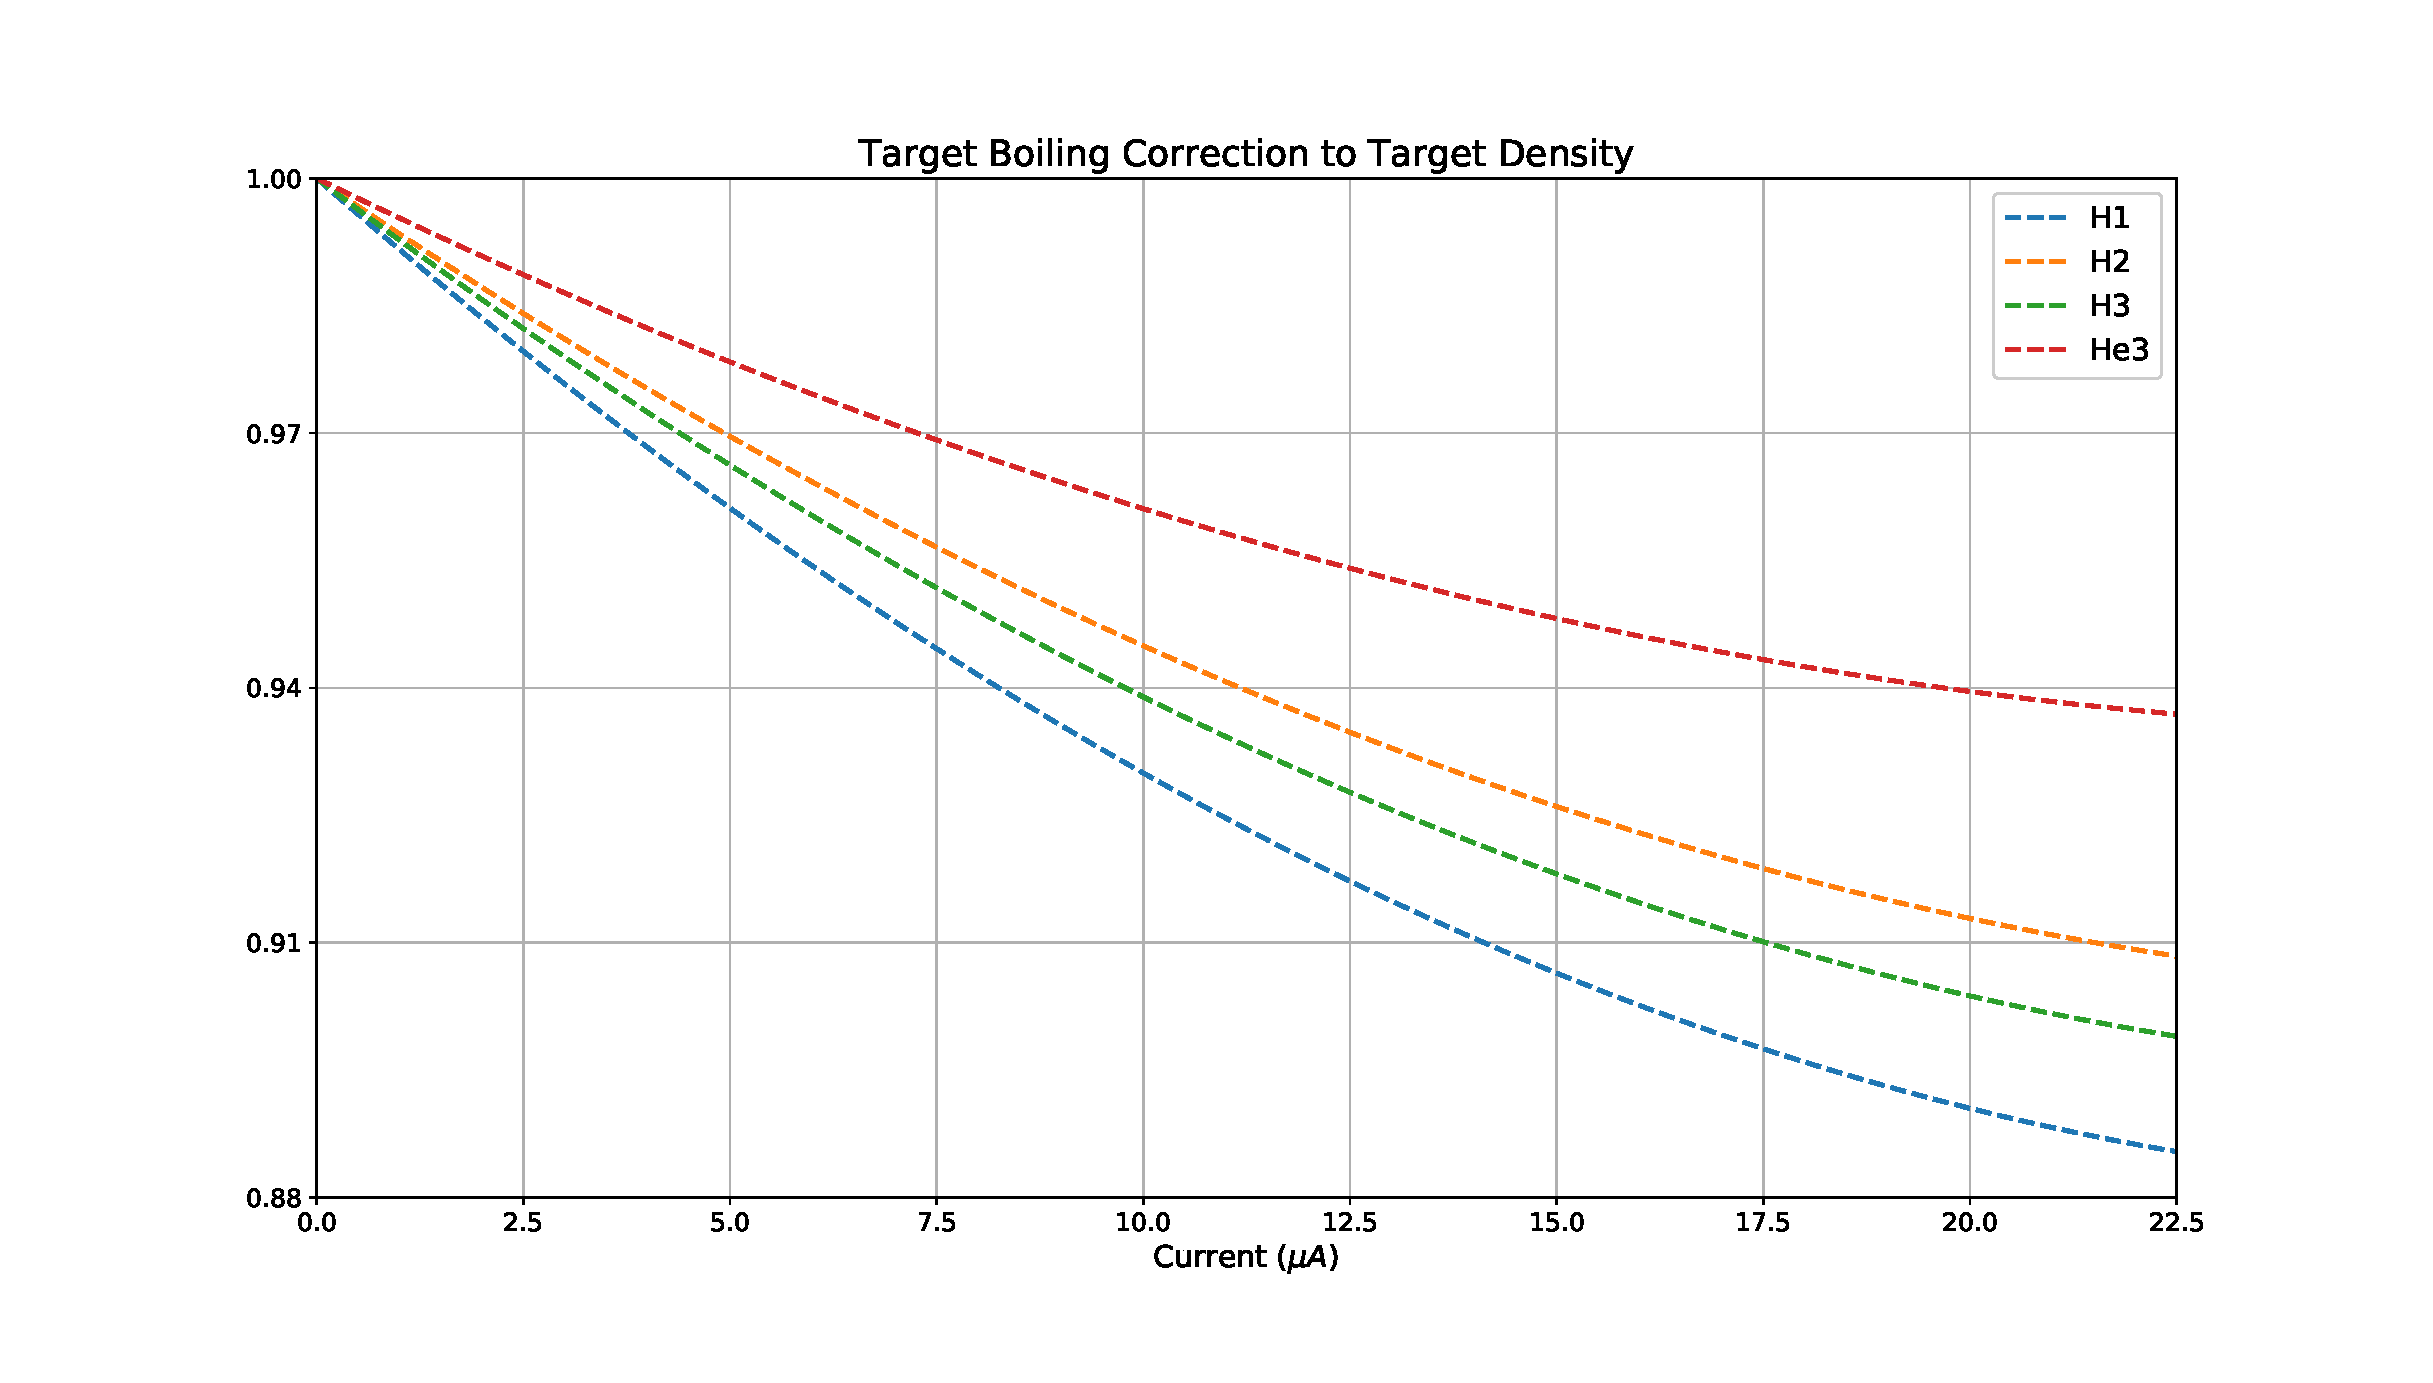
\includegraphics[width=\textwidth]{./analysis/fig/boil_cor.eps}
	\caption{Beam heating effects are manifested as a multiplicative correction to the target density}
	\label{fig:boilcor}
\end{figure}

%\begin{figure}
%	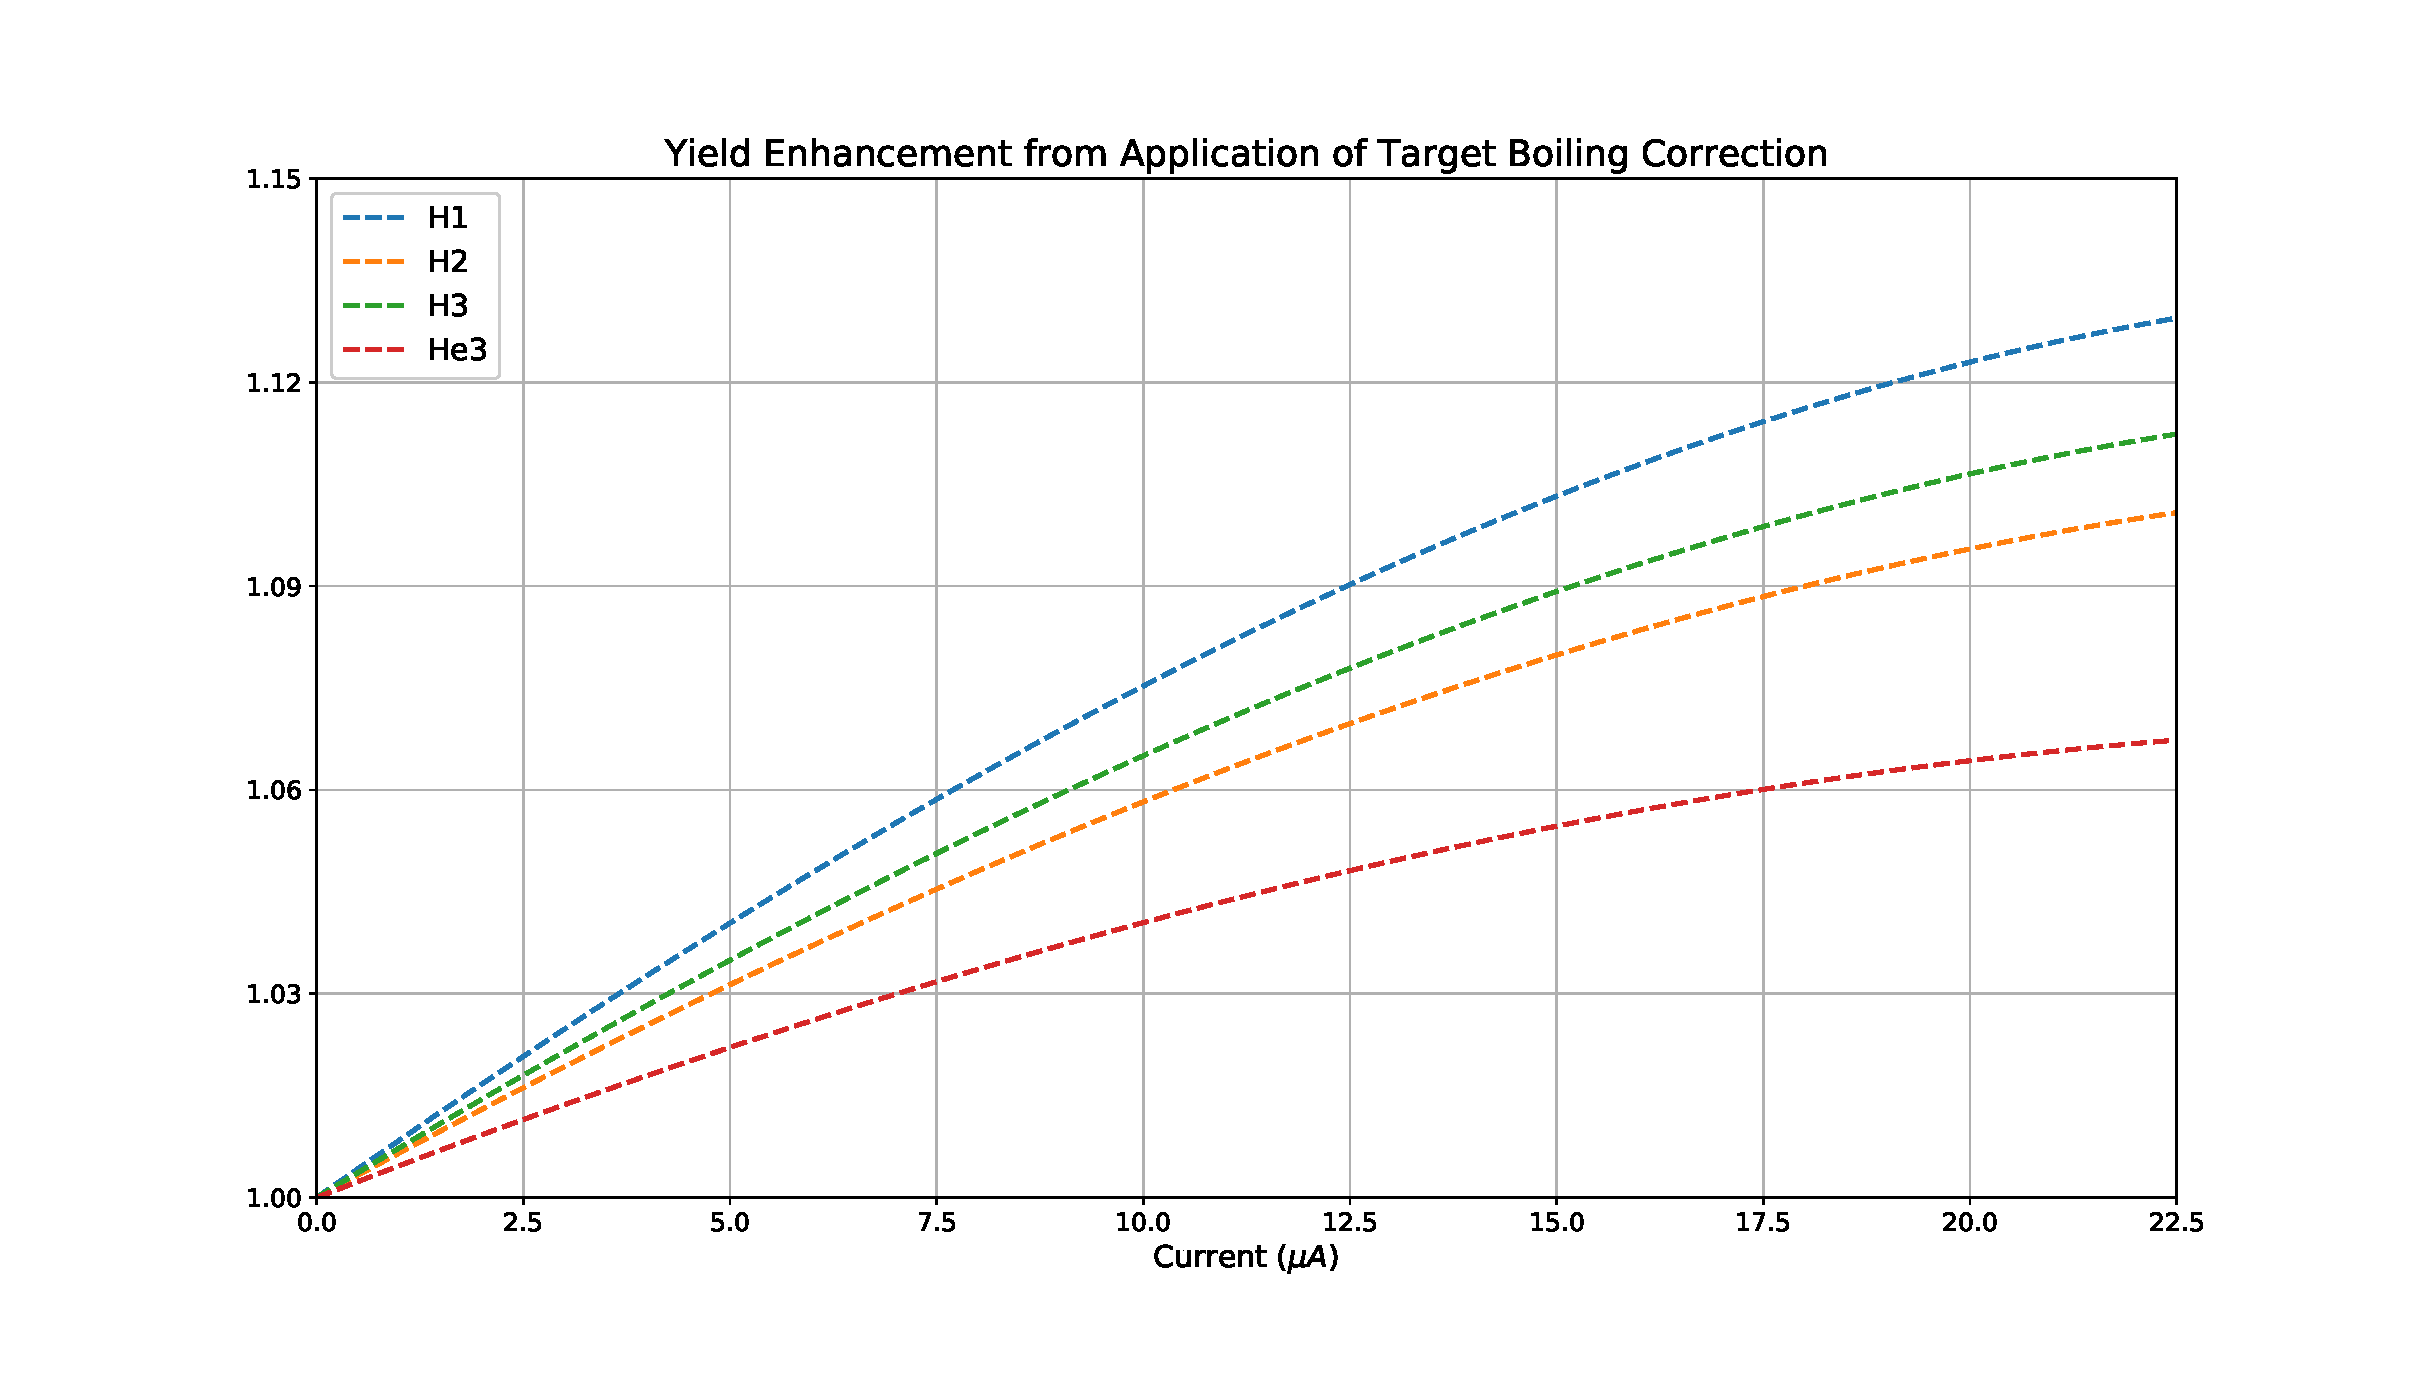
\includegraphics[width=\textwidth]{./analysis/fig/boil_yield_cor.eps}
%	\caption{Target density corrections cause a multiplicative enhancement to the yield}
%	\label{fig:boilyieldcor}
%\end{figure}

\subsection{Target Endcap Contamination}
\label{sec:ecc}

The gas targets used in this experiment are housed in aluminum cells as described in Section \ref{sec:gas_cell}. The thickness of the aluminum greatly exceeds the thickness of the gas and will contribute background that can survive the cuts placed on the data. By quantifying this contribution, the events that originate from the cell endcaps can be subtracted from the final results.

To determine this contribution, the empty cell is used. The empty cell, being an exact replica of the gas target cells with a vacuum inside, allows us to approximately isolate the contribution of the cell walls to the data. The empty cell and the target being studied are compared by calculating the yields on a kinematic-by-kinematic basis and normalizing them by charge and endcap thickness.

The normalization to the endcaps for each target must be done in two parts. This is because each endcap is not the same thickness. When calculating the yield for a target, it is assumed that any contamination upstream (downstream) of the center of the target must originate from the upstream (downstream) endcap. The two halves are then combined to arrive at the endcap thickness normalized yield. This yield calculation only has livetime corrections applied. All cuts are applied except for target length, which is adjusted to only include events upstream (downstream) of the center of the target.

The data for the target being studied and the normalized empty target are then binned in Bjorken $x$. Dividing the empty cell data by the gas target data then gives an approximation of the fractional contribution of the cell walls to the electron data. As this correction is applied to the final results, the contamination corrections for the targets are divided by each other to create the correction to the target ratios. These results are then fit with the functional form $1\pm e^{Ax+B}$. The choice of adding or subtracting the exponential is done by determining if the correction is greater or smaller than 1. The fit function and the covariance matrix of the fit are used to apply the correction to the final results as well as determine the uncertainty contribution of this correction.

\subsection{Charge Symmetric Background Subtraction}

As an inclusive scattering experiment, we are particularly susceptible to background from charge symmetric processes from the target. That is events which involved the production of both an electron and a positron, rather than the electron simply scattering. To study this, the polarity of the LHRS was reversed so that positively charge particles are directed into the detectors rather than negatively charged particles. With this setting, a number of runs were taken in kinematics 0 through 5. These runs were taken with all targets, just as the electron data was taken. This allows for a measurement of the positron yield which corresponds to a measure of the charge symmetric background.

This measurement allows us to determine the proportion of electrons that originated from pair production. Applying the same cuts and as the electron data allows us to determine the charge normalized positron yield. Unlike in the electron analysis, it was noted that there was significant pion contamination in the positron data. This pion contamination had to be subtracted in order to get an accurate calculation of the positron yield. This is achieved by fitting the main pion peak and the subtracting the tail of the fit which survives the cuts applied from the positron data.

The charge normalized positron yields over these kinematics are then combined (using the same methods as the electron yield) and binned in Bjorken $x$. This was then divided by the charge normalized electron yield. This is a fractional measure of the charge normalized background contamination. The ratio is then fit with an exponential of the form $e^{Ax + B}$, where $A$ and $B$ are the fit parameters. These fits are shown in in Figure \ref{fig:positrons}.

This correction is applied to the final yield ratio results. Both the numerator and denominator must have the charge symmetric background subtracted. Each target yield in the ratio is scaled by $1 - \left(\textrm{Charge Symmetric Background Fit}\right)$. For each bin, the fit is calculated at the bin center.

\begin{figure}
	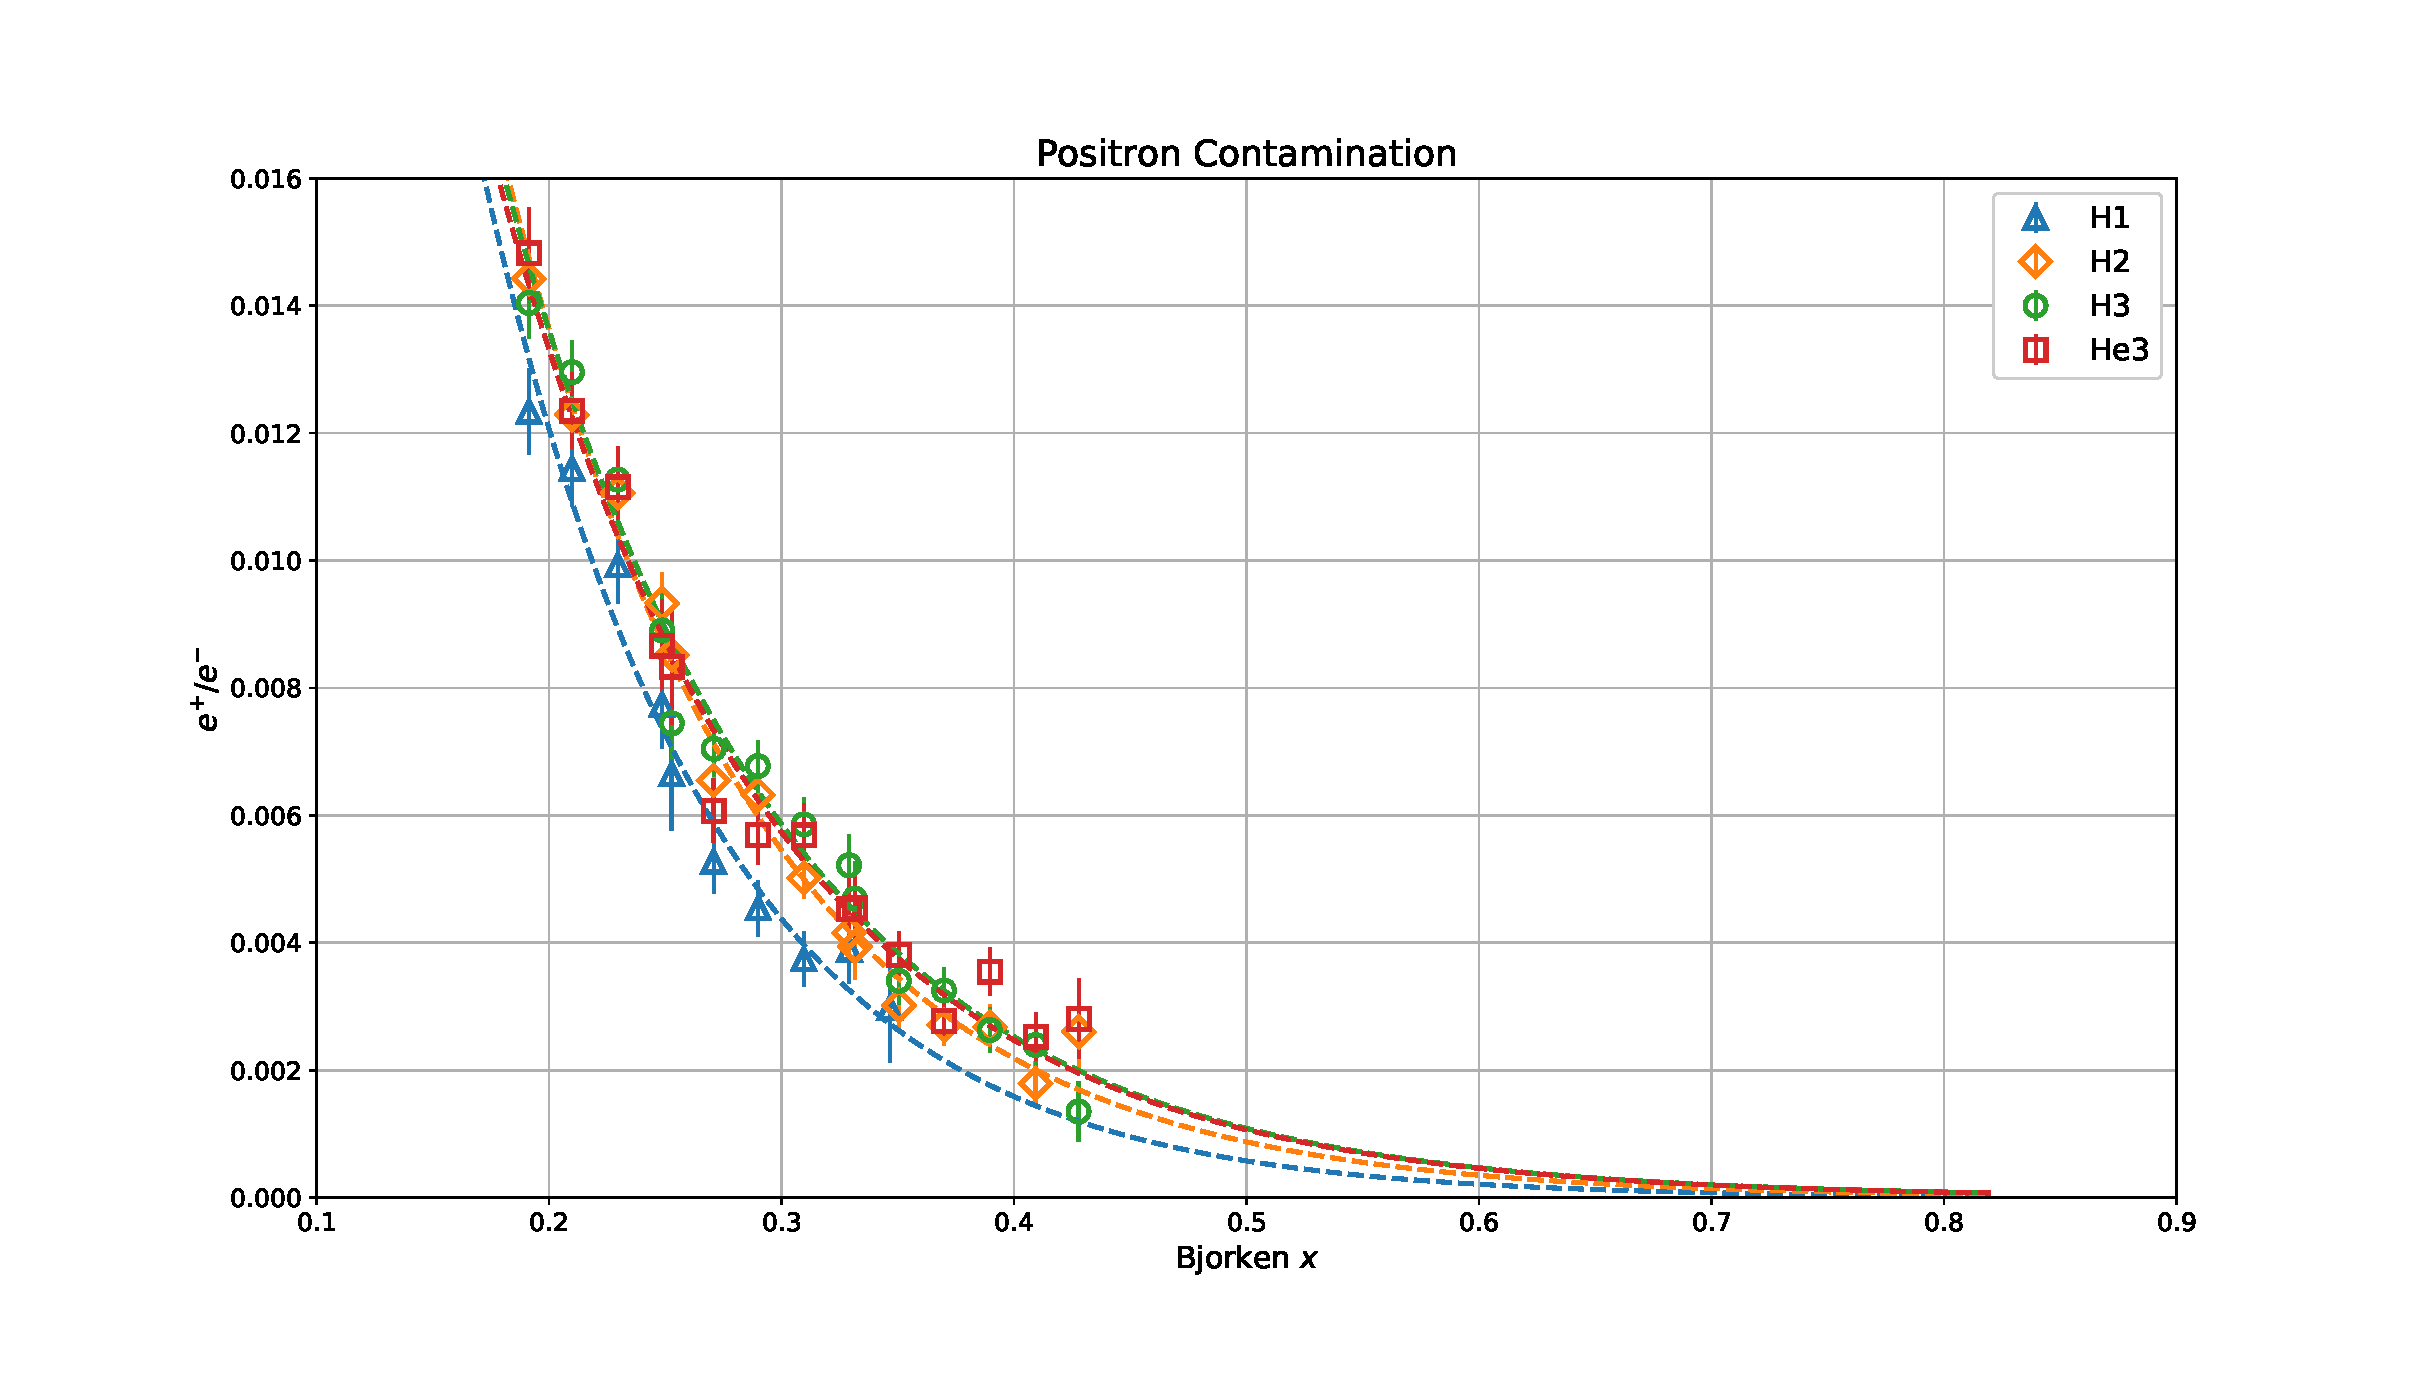
\includegraphics[width=\textwidth]{./analysis/fig/positrons.eps}
	\caption{Charge symmetric background correction}
	\label{fig:positrons}
\end{figure}

\subsection{Computer Deadtime Correction}

Our DAQ unable to continuously record data. While we can probabilistically determine the mean time spacing between events, in the real world events can deviate greatly from these means. Sometimes events will occur that are too close in time for our DAQ to record as the computer has not completed recording the previous event. Deadtime is a function of event rate; when events happen more rapidly, there is a higher chance that events will occur too closely in time to be recorded.

When deadtime is low and the number of recorded events is high, it is a reasonable assumption that the events recorded will accurately reflect the distribution of events in the ``zero-deadtime limit''. In this case correcting for the deadtime is simply done by scaling the number of events by the ``livetime'' of the experiment.

The computer livetime was measured using the Trigger Supervisor and scalers in each HRS. The trigger signals generated from detector signals are copied and sent to both the Trigger Supervisor and a scaler unit. The Trigger Supervisor is subject to the computer deadtime event loss discussed here. The scaler unit, on the other hand, simply increments a register when a trigger signal is received. The ratio of these the number of events recorded by these two systems gives a measure of the livetime of the measurement. The livetime is defined on a run-by-run basis as:

\begin{equation}
DT = \frac{\Sigma \mathrm{Triggers_{TS}}}{\Sigma \mathrm{Triggers_{Scaler}}}
\end{equation}

In an ideal world, the deadtime will be identical for all runs within a kinematic. However, the deadtime is measured on a run-by-run basis and is applied as such in order to account for any deviations from this assumption. The average deadtime for each target in each kinematic is plotted in Figure \ref{fig:deadtime}.

\begin{figure}
	\includegraphics[width=\textwidth]{./analysis/fig/deadtime.eps}
	\caption{Deadtime per kinematic}
	\label{fig:deadtime}
\end{figure}

\subsection{Radiative Corrections}

The Deep Inelastic Cross Sections being studied are the Born approximation of a single-photon exchange. The measurement however, contains contributions from higher order processes that will increase the measured cross section. Using a model, the contributions can be corrected for and removed from the measurement.

The experiment used a software package called $\texttt{T2\_EXTERNALS}$ that calculates both the Born cross section and the radiated cross section for a given target at a kinematic set $(E,E^{\prime} ,\theta )$.

\subsection{Isoscalar Corrections}

\subsection{Bin Centering Corrections}

The cross-section over the width of a bin is not constant. This means that the measurement does not correspond with the true cross section at the center of the bin. Using a model that matches the shape of our data well, the location of the measurement within the bin can be calculated. This is done by calculating the expectation value of the model within that bin and determining the $x$ value corresponding to this value. The expectation value is given by
\begin{equation}
	\langle f_{\rm measured}\rangle = \frac{1}{\Delta x}\int_{x_{\rm low}}^{x_{\rm high}} f\left( x \right) dx,
\end{equation}
where $f$ is a function representing the chosen model. In practice, the $x$ value does not need to be calculated if the data will be reported at the bin center. Rather, the correction is simply the ratio of the model at the bin center. This is written as
\begin{equation}
	\sigma_{\textrm{Bin Centered}} = \frac{f\left(x_{\textrm{Bin Center}}\right)}{\langle f_{\rm measured}\rangle} \sigma_{\rm measured}.
\end{equation}

This correction must be applied to both targets in the ratios. That is, the ratio must be multiplied by the correction to the numerator and divided by the correction to the denominator.\cite{wtsydp}

\subsection{Coulomb Corrections}

Corrections must be made for the effect of the charge of the target on the scattered electron. This interaction causes the $Q^2$ of the event to shift to an effective $Q^2$ value, $Q^2_{\rm eff}$. This conversion is done with the equation
\begin{equation}
	Q^2_{\rm eff} = Q^2 \left(1 + \frac{3Z\alpha\hbar c}{2RE}\right)^{2}.
\end{equation}
In this equation $R$ is the hard-sphere equivalent radius of the nucleus which is defined as $R=\left[\left(\nicefrac{5}{3}\right) \langle r^{2}\rangle\right]^{\nicefrac{1}{2}}$ where $\langle r^2\rangle$ is the root-mean-squared radius of the nucleus.\cite{coulomb}

Using $x=\frac{Q^2}{2M\nu}$, it is clear that a shift in $Q^2$ will result in a proportional shift in $x$. Using a model cross-section, the cross section is calculated at both the nominal $x$ and at $x_{\rm eff}$. As the results have been bin centered, this calculation uses a nominal $x$ at the center of the bin. This will lead to the correction
\begin{equation}
	\sigma_{\textrm{Coulomb Corrected}} = \sigma_{\rm data} \frac{\sigma_{\rm model}\left(x_{\rm eff}\right)}{\sigma_{\rm model}\left(x\right)}.
\end{equation}

This correction must be applied to both targets in the ratios that are calculated.
\subsection{Particle Identification}


\chapter{\bf{Results}}    % Chapter  4
\setcounter{figure}{0}
\setcounter{table}{0}
\setcounter{equation}{0}
%\section{Title of First section}
%
%
%\subsection{First subsection}
%
%Here is a Table....
%
%\begin{table}[ht!]
%\caption{Forward Electron Scattering Run Plan}
%\begin{center}
%\begin{tabular}{cccccccc}
%%\multicolumn {7} {c}  {\bf TABLE 4} \\
%\multicolumn {7} {c}  {\bf FORWARD ELECTRON SCATTERING RUN PLAN } \\
%\multicolumn {7} {c}  { } \\ \hline
%$Q^2$  &  $F_C$  & $F_M$ &Cross Section & Time  & Counts & $\Delta F_C$ \\
% (fm$^{-2}$)  &  &  & (cm$^2$/sr) & (hr)  &  & ($\pm\%$) \\ \hline
%    &                     &                     &                           &     &     \\
%12.90 & 3.0$\times 10^{-4}$ & 8.0$\times 10^{-3}$ & 2.7$\times 10^{-34}$ & 1.2 & 12240 & NM  \\
%15.50 & 3.0$\times 10^{-3}$ & 3.4$\times 10^{-3}$ & 5.9$\times 10^{-35}$ & 4.8 & 10800 & 13 \\
%17.50 & 3.5$\times 10^{-3}$ & 1.8$\times 10^{-3}$ & 3.0$\times 10^{-35}$ & 1.2 & 1380  & 9.5 \\
%20.00 & 3.3$\times 10^{-3}$ & 7.0$\times 10^{-4}$ & 1.5$\times 10^{-35}$ & 2.4 & 1360  & 4.1 \\
%22.80 & 2.8$\times 10^{-3}$ & 6.0$\times 10^{-5}$ & 1.4$\times 10^{-35}$ & 1.2 & 630   & 5.4 \\
%26.00 & 2.2$\times 10^{-3}$ & 3.0$\times 10^{-4}$ & 6.4$\times 10^{-36}$ & 4.8 & 1175  & 3.1 \\
%28.00 & 1.8$\times 10^{-3}$ & 4.7$\times 10^{-4}$ & 4.4$\times 10^{-36}$ & 2.4 & 395   & 5.2 \\
%31.50 & 1.3$\times 10^{-3}$ & 5.0$\times 10^{-4}$ & 2.2$\times 10^{-36}$ & 12  & 990   & 11 \\
%35.00 & 9.0$\times 10^{-4}$ & 4.2$\times 10^{-4}$ & 9.9$\times 10^{-37}$ & 9.6 & 360   & 17 \\
%39.25 & 5.5$\times 10^{-4}$ & 3.0$\times 10^{-4}$ & 3.5$\times 10^{-37}$ & 12  & 160   & 25 \\
%43.00 & 3.2$\times 10^{-4}$ & 1.9$\times 10^{-4}$ & 1.1$\times 10^{-37}$ & 19  & 83    & 35 \\
%47.50 & 2.0$\times 10^{-4}$ & 1.1$\times 10^{-4}$ & 3.4$\times 10^{-38}$ & 12  & 16    & NM \\
%Total      &                  &                     &                      & 83  &      &    \\
%           &                  &                     &                      &     &      &  \\ \hline
%\end{tabular}
%\end{center}
%%\caption{Run plan scenario with cross section
%%and counting rate estimates for the forward electron scattering measurements, using the
%%Left HRS system to detect scattered electrons and the BigBite spectrometer to detect
%%recoil triton nuclei in coincidence. (NM means not measurable).}
%\label{table:frp}
%\end{table}
%
%Here is a second Table....
%
%\begin{table}[ht!]
%\caption{Backward Electron Scattering Run Plan}
%%\caption{Backward Electron Scattering Run Plan}
%\begin{center}
%\begin{tabular}{cccccccc}
%%\multicolumn {7} {c}  {\bf TABLE 4} \\
%\multicolumn {7} {c}  {\bf BACKWARD ELECTRON SCATTERING RUN PLAN } \\
%\multicolumn {7} {c}  { } \\ \hline
%$Q^2$  &  $F_C$  & $F_M$ &Cross Section & Time  & Counts & $\Delta F_M$ \\
% (fm$^{-2}$) &  &  & (cm$^2$/sr) & (hr)  &  & ($\pm\%$) \\ \hline
%    &                     &                     &                           &     &     \\
%12.90 & 3.0$\times 10^{-4}$ & 8.0$\times 10^{-3}$ & 9.7$\times 10^{-36}$ & 0.6 & 1080 & 5.2  \\
%15.50 & 3.0$\times 10^{-3}$ & 3.4$\times 10^{-3}$ & 1.7$\times 10^{-36}$ & 2.4 & 885 & 5.6 \\
%17.50 & 3.5$\times 10^{-3}$ & 1.8$\times 10^{-3}$ & 5.8$\times 10^{-37}$ & 0.6 & 86  & 4.6 \\
%20.00 & 3.3$\times 10^{-3}$ & 7.0$\times 10^{-4}$ & 1.7$\times 10^{-37}$ & 4.8 & 226  & 25 \\
%22.80 & 2.8$\times 10^{-3}$ & 6.0$\times 10^{-5}$ & 4.5$\times 10^{-38}$ & 0.6 & 10   & NM \\
%26.00 & 2.2$\times 10^{-3}$ & 3.0$\times 10^{-4}$ & 1.5$\times 10^{-38}$ & 8.5 & 50  & 26 \\
%28.00 & 1.8$\times 10^{-3}$ & 4.7$\times 10^{-4}$ & 1.5$\times 10^{-38}$ & 3.6 & 22   & 15 \\
%31.50 & 1.3$\times 10^{-3}$ & 5.0$\times 10^{-4}$ & 3.7$\times 10^{-38}$ & 4.8  & 48   & 21 \\
%35.00 & 9.0$\times 10^{-4}$ & 4.2$\times 10^{-4}$ & 1.8$\times 10^{-38}$ & 6.0 & 30   & 19 \\
%39.25 & 5.5$\times 10^{-4}$ & 3.0$\times 10^{-4}$ & 6.5$\times 10^{-39}$ & 8.5 & 19   & 18 \\
%43.00 & 3.2$\times 10^{-4}$ & 1.9$\times 10^{-4}$ & 2.1$\times 10^{-39}$ & 15  & 12    & 19 \\
%47.50 & 2.0$\times 10^{-4}$ & 1.1$\times 10^{-4}$ & 5.5$\times 10^{-40}$ & 17  & 4 & 27 \\
%Total      &                  &                     &                      & 72  &      &    \\
%           &                  &                     &                      &     &      &  \\ \hline
%\end{tabular}
%\end{center}
%%\caption{Run plan scenario with cross section
%%and counting rate estimates for the backward electron scattering measurements, using {\it both}
%%HRS systems to detect recoil tritons.
%%The run plan assumes for $Q^2 \ge 2.5$~ (GeV/{\it c})$^2$ a form factor behavior
%% (NM means not measurable).}
%\label{table:brp}
%\end{table}
%
%\subsection{Second subsection}
%
%\subsection{Third subsection}
%


%----------------------------------------------------------------------------


\appendix
\chapter{Title of Appendix A}
\setcounter{figure}{0}
\setcounter{table}{0}
\setcounter{equation}{0}
%\section{Title of section 1 of Appendix A}
%
%This will be Appendix A.
%\section{Title of section 2 of Appendix A}
%
%Some paragraphs ......\\
%
%
%More paragraphs ...


%----------------------------------------------------------------------------


%\input{diss.bbl}
\begin{thebibliography}{100}
%\begin{thebibliography}{99}


\vskip-0.6in
\bibitem{mara} {\it Measurement of the $F_2^n/F_2^p$ and $d/u$ ratios and $A=3$ EMC
effect in deep inelastic scattering off the tritium and helium mirror nuclei},
JLab Proposal PR-12-10-103, J.~Arrington et al., The JLab MARATHON Collaboration, 2010.
\bibitem{CA97} C.~E.~Carlson, J.~R.~Hiller and R.~J.~Holt, Annu. Rev. Nucl.
               Part. Sci. {\bf 47}, 395 (1997).
\bibitem{AL99} L.~C.~Alexa {\it et al.}, Phys. Rev. Lett. {\bf 82},
               1374 (1999); and references therein.
\bibitem{CA13} A.~Camsonne {\it et al.}, {\it Measurement of the $^4$He charge
               form factor at large momentum transfers at Jefferson Lab}, to be
               submitted to Phys. Rev. Lett., May 2013.
\bibitem{KA86} A.~T.~Katramatou, SLAC Report SLAC-NPAS-TN-86-08 (1986).      
\bibitem{PE86} G.~G.~Petratos, SLAC Report NPAS-TN-86-07 (1986).
\bibitem{KA88} A.~T.~Katramatou {\it et al.},
               Nucl. Instrum. Meth. {\bf A267}, 448 (1988).
\bibitem{RITH} K. Rith. 1997. \textit{Lectures on QCD: Applications}. Berlin, Heidelberg: Springer Berlin Heidelberg. \textit{Quark-Gluon Structure of the Nucleon}; p. 250-346.
\bibitem{HaM} F. Halzen, A. Martin. 1984. \textit{Quarks and Leptons: An Introductory Course in Modern Particle Physics}. Wiley.
               
%@Inbook{Rith1997,
%author="Rith, K.",
%editor="Lenz, Frieder
%and Grie{\ss}hammer, Harald
%and Stoll, Dieter",
%title="Quark-gluon structure of the nucleon",
%bookTitle="Lectures on QCD: Applications",
%year="1997",
%publisher="Springer Berlin Heidelberg",
%address="Berlin, Heidelberg",
%pages="250--346",
%isbn="978-3-540-46967-4",
%doi="10.1007/BFb0105861",
%url="http://dx.doi.org/10.1007/BFb0105861"
%}

         
               
%\end{thebibliography}




\end{thebibliography}
\bibliographystyle{unsrt}
\bibliography{bibliography}

%%% need file ksudiss.sty and report.sty
%% remove leqno to get equation numbers on the right side!
%%\documentstyle[leqno,12pt]{ksudiss}
\documentclass[12pt,leqno]{ksudiss}
\usepackage{verbatim,epsfig,amstext,amsmath,amssymb,float,afterpage,graphicx,graphics, epstopdf, gensymb,tabulary,nicefrac}

\title{Super Awesome MARATHON Thesis}
\author{Tyler Hague}
\namedegreedate{Tyler Hague}
\pages{}
\advisor{MK MP}

\degrees{B.S., Abilene Christian University, 2012\\
     M.S/ Ph.D.,  Kent State University, TBD}
%\figurespagefalse  % need to put % in front of \ to get figure index
%\tablespagefalse   % need to put % in front of \ to get table index
\newcommand{\cdate}{November, 2016}  %month, year need to be changed
\makeindex   % - uncomment if index needed
%% these are some local definition - use only if needed

\newcommand{\Notequiv}{/\kern-.6em\hbox{$\equiv$}}
\newcommand{\Ceals}{\rm I\kern-.5emC}
\newcommand{\nsubset}{/\kern-.6em\hbox{$\subset$}}
\newcommand{\dis}{\displaystyle}
\newcommand{\nin}{\backslash \kern-.5em\in}
\newcommand{\Index}[1]{#1\index{#1}}
%\newcommand{\dedx}{\mbox{$\langle dE/dx \rangle$}\index{dedx@$dE/dx$}}
\newcommand{\pt}{p_{\rm T}}
\newcommand{\mt}{m_{\rm T}}
\renewcommand{\thefigure}{\thechapter.\arabic{figure}}
\renewcommand{\thetable}{\thechapter.\arabic{table}}
\renewcommand{\theequation}{\thechapter.\arabic{equation}}

\newcommand{\beqn}{\begin{equation}}
\newcommand{\eeqn}{\end{equation}}
%% end of local definitions


%----------------------------------------------------------------------------


\begin{document}

\restylefloat{table}
\restylefloat{figure}

%\abstract
%\input{abstract_colloq.tex}


%---------------------------------------------------------------------------
\abstract

This is the abstract file abstract.tex\\

My research field is experimental nuclear physics.  My work was  ------


We present the details of the  analysis, the obtained distributions, and their discussion.

MARATHON is a Deep Inelastic Scattering experiment in Jefferson Lab's Hall A. The experiment utilized Deuterium, Helium-3, and Tritium targets to extract the $F_2^n/F_2^p$ structure function ratio and R. \textbf{Need to give an explanation of R. Talk about EMC and why we're looking at these things. Mention uniqueness of having Tritium target}

\frontmatter 
\submitdate{March 2015}


%----------------------------------------------------------------------------


\prefacesection{Acknowledgments}
This is the acknowledgements text.

%----------------------------------------------------------------------------


\startthesis
%\psdraft

\chapter{\bf{Introduction}}
\setcounter{figure}{0}
\setcounter{table}{0}
\setcounter{equation}{0}
%Prior to \textbf{EMC EFFECT STUFF} it was taken for granted that quark distributions were independent of the surrounding nucleus. The European Muon Collaboration (EMC) found this not to be the case. They found that quark distributions are different in a nucleus than in a nucleon. The ratio of the Iron to Deuterium $F_2$ structure functions was found to greatly deviate from unity.
%
%EMC EMC EMC. $A=3$ nuclear structure data is critical to understanding the nature of the EMC effect.
%
%The MARATHON experiment studied the cross section ratios of the He3/H2, H3/H2, H3/He3. This data aims to provide a more complete understanding of the EMC effect and nuclear structure. In this thesis, I will describe the analysis of the He3 EMC effect. The next two chapters will provide an overview of electron-nucleon Deep Inelastic Scattering and the EMC effect. Chapter 4 will describe the experimental setup used in Hall A of Thomas Jefferson National Accelerator Facility (JLab). Chapter 5 will go over the analysis of the cross section ratio. Finally, Chapter 6 will present the results of my analysis.

%%%%%%

A pioneering experiment at Stanford Linear Accelerator Center (SLAC) \cite{SLAC_DIS} showed that, at sufficiently high momentum transfer, lepton scattering is sensitive to the partonic structure of the nucleon. This led to a renaissance of scattering experiments, all vying to better our understanding of nuclear structure and the constituent parts that make up the nucleus. High momentum transfer scattering, dubbed Deep Inelastic Scattering (DIS), has proven to be an invaluable tool for the study of nuclear physics.

One puzzle still unsolved, born out of the use of DIS to study the nuclear structure functions, is that of the EMC effect. The European Muon Collaboration, the namesake of the EMC effect, studied the ratio of the per nucleon cross-sections of Iron (corrected for neutron excess) to Deuterium in an effort to understand their experimental systematics \cite{emc_FE}. What was found was clear evidence for nucleon modification within the nucleus. Where they expected a measurement of unity, the ratio exhibited a downward slope in the region of the data. This is the EMC effect.

Since then, many experiments have contributed data sets to the study of the EMC effect. These data have shown correlations between the strength of the EMC effect and various nuclear quantities, such as mass number $A$, nuclear density, and short range correlations within the nucleus. The available measurements have primarily focused on heavy nuclei, with the exception of the JLab E03-103 experiment which focused on light nuclei.

The MARATHON experiment ran in Hall A of Thomas Jefferson National Accelerator Facility (JLab) using a $10.59\ \text{GeV}$ electron beam from the CEBAF accelerator. One of the primary goals for MARATHON was to measure the EMC effect in the $A=3$ mirror nuclei, $^3$He and $^3$H \cite{proposal}. The measurement of the $A=3$ EMC effects are considered critical to a more complete understanding of the EMC effect. This thesis will present the study of the $^3$He EMC effect from the MARATHON data. Chapter \ref{chap:scattering} will give an overview of electron scattering with a focus on Deep Inelastic Scattering. Chapter \ref{chap:emc} will discuss the history of the EMC effect, as well as a selection of models that aim to describe it. Chapter \ref{chap:setup} describes the experimental setup of the MARATHON experiment at JLab. Chapter \ref{chap:analysis} shows the methods used to analyze the data acquired from the experiment. Finally, Chapter \ref{chap:results} presents the results of this study, as well as a look into how the measured strength of the $^3$He EMC effect fits in with correlations that are useful for understanding the source of this effect.

\chapter{\bf{Electron Scattering and Nuclear Structure}}             % Chapter  1
\setcounter{figure}{0}
\setcounter{table}{0}
\setcounter{equation}{0}
\section{Yield Calculation}

The MARATHON experiment measured cross section ratios. This method allows us to cancel many systematics that would otherwise plague a full cross section analysis. By taking data for each target at the same kinematics, acceptance effects are identical. This data taking technique means that with reasonable acceptance cuts, a ratio of target yields is wholly equivalent to the ratio of cross sections.

To calculate the yield we use a simple equation:

\begin{equation}
	\text{Yield} = \frac{\text{Counts}}{\text{Scattering Centers} \cdot \text{Livetime}} \cdot \text{Corrections}
\end{equation}

The yield is binned in Bjorken $x$. This chapter will explain the cuts and corrections that go into this calculation.

\section{Calibration}
\input{./chap3-analysis/calib.tex}

\section{Analysis}
\input{./chap3-analysis/corrections.tex}
\subsection{Particle Identification}


\chapter{\bf{The EMC Effect}}             % Chapter  1
\setcounter{figure}{0}
\setcounter{table}{0}
\setcounter{equation}{0}
\section{Yield Calculation}

The MARATHON experiment measured cross section ratios. This method allows us to cancel many systematics that would otherwise plague a full cross section analysis. By taking data for each target at the same kinematics, acceptance effects are identical. This data taking technique means that with reasonable acceptance cuts, a ratio of target yields is wholly equivalent to the ratio of cross sections.

To calculate the yield we use a simple equation:

\begin{equation}
	\text{Yield} = \frac{\text{Counts}}{\text{Scattering Centers} \cdot \text{Livetime}} \cdot \text{Corrections}
\end{equation}

The yield is binned in Bjorken $x$. This chapter will explain the cuts and corrections that go into this calculation.

\section{Calibration}
\input{./chap3-analysis/calib.tex}

\section{Analysis}
\input{./chap3-analysis/corrections.tex}
\subsection{Particle Identification}


\chapter{\bf{The Experiment}}    % Chapter  2
\setcounter{figure}{0}
\setcounter{table}{0}
\setcounter{equation}{0}
\section{The Measurement}
\subsection{What are we measuring}
\subsection{How are we measuring it}
\subsection{Run Plan}

\section{The Apparatus}
\subsection{Hall A HRS Spectrometers}
\subsection{CEBAF Accelerator}

% \chapter{\bf{Chapter 2 Title}    % Chapter  2
%Introductory paragraph of Chapter 2.......
%
%\section{First section Title}
%
%First section text......
%
%
%
%\subsection{First Subsection Title}
%
%
%The cross section for elastic electron scattering from the spin one-half
%$^3$H  nucleus is given, in the one-photon exchange approximation, by:
%\beqn
%{  {d\sigma} \over {d\Omega} } (E,\Theta)  =
%{  {(Z\alpha)^2 E^\prime} \over {4 E^3  \sin^4 \left( {\Theta \over 2} \right)}  }
%\left[ A(Q^2) \cos^2 \left( {\Theta \over 2} \right) +
%B(Q^2) \sin^2 \left( {\Theta \over 2} \right) \right],
%\label{morefequ}
%\eeqn
%where $Z$ is the nuclear charge, $\alpha$ is the fine-structure constant,
%$E$ and $E'$ are the incident and scattered electron energies,
%$\Theta$ is the electron scattering angle, $Q^2 = 4 E E' \sin^2 (\Theta/2)$ is
%minus the squared four-momentum transfer,
%and $A(Q^2)$ and $B(Q^2)$ are the $^3$H elastic structure functions, given in
%terms of the charge and magnetic form factors as:
%\beqn
%{   A(Q^2) = {   { F^2_C(Q^2) +
%(1+\kappa)^2 \tau F^2_M(Q^2) } \over {1 + \tau} }    },
%\label{more1}
%\eeqn
%\beqn
%{ B(Q^2) =  2 \tau (1+\kappa)^2 F^2_M(Q^2) },
%\label{more2}
%\eeqn
%where
%$\tau=Q^2/4M^2$ with $M$ being the mass of the target nucleus, and
%$\kappa$ is the anomalous magnetic moment of the nucleus.
%
%Here is a reference ~\cite{mara} which needs to be defined in the bibliography.tex file first.
%
%
%Here comes a Figure....
%
% \begin{figure}[!htbp]
%  \begin{center}
%    \includegraphics[angle=90, scale=0.65]{./chap2-exp/fig/tritium_past.eps}
%  \end{center}
%  \caption[Tritium Magnetic Form Factor Past Data]{
%    \footnotesize Tritium Mag. Form Factor past data.
%  }
%  \label{fig:TritiumM}
%\end{figure}
%
%Use the label name to refer to  Figure  ~\ref{fig:TritiumM}.
%
%
%\subsection{Second Subsection  Title}
%
%Subsection text..........
%
%
%
%\subsubsection{First Subsubsection}
%
%This is a subsubsection.
%
%
%
%\subsubsection{Second Subsubsection}
%
%This another  subsubsection.

\setcounter{figure}{0}
\setcounter{table}{0}
\setcounter{equation}{0}
\subsection{Raster}
\input{./chap2-exp/raster.tex}


\chapter{\bf{Analysis}}    % Chapter  3
\setcounter{figure}{0}
\setcounter{table}{0}
\setcounter{equation}{0}
\section{Yield Calculation}

The MARATHON experiment measured cross section ratios. This method allows us to cancel many systematics that would otherwise plague a full cross section analysis. By taking data for each target at the same kinematics, acceptance effects are identical. This data taking technique means that with reasonable acceptance cuts, a ratio of target yields is wholly equivalent to the ratio of cross sections.

To calculate the yield we use a simple equation:

\begin{equation}
	\text{Yield} = \frac{\text{Counts}}{\text{Scattering Centers} \cdot \text{Livetime}} \cdot \text{Corrections}
\end{equation}

The yield is binned in Bjorken $x$. This chapter will explain the cuts and corrections that go into this calculation.

\section{Calibration}
\input{./chap3-analysis/calib.tex}

\section{Analysis}
\input{./chap3-analysis/corrections.tex}
\subsection{Particle Identification}


\chapter{\bf{Results}}    % Chapter  4
\setcounter{figure}{0}
\setcounter{table}{0}
\setcounter{equation}{0}
%\section{Title of First section}
%
%
%\subsection{First subsection}
%
%Here is a Table....
%
%\begin{table}[ht!]
%\caption{Forward Electron Scattering Run Plan}
%\begin{center}
%\begin{tabular}{cccccccc}
%%\multicolumn {7} {c}  {\bf TABLE 4} \\
%\multicolumn {7} {c}  {\bf FORWARD ELECTRON SCATTERING RUN PLAN } \\
%\multicolumn {7} {c}  { } \\ \hline
%$Q^2$  &  $F_C$  & $F_M$ &Cross Section & Time  & Counts & $\Delta F_C$ \\
% (fm$^{-2}$)  &  &  & (cm$^2$/sr) & (hr)  &  & ($\pm\%$) \\ \hline
%    &                     &                     &                           &     &     \\
%12.90 & 3.0$\times 10^{-4}$ & 8.0$\times 10^{-3}$ & 2.7$\times 10^{-34}$ & 1.2 & 12240 & NM  \\
%15.50 & 3.0$\times 10^{-3}$ & 3.4$\times 10^{-3}$ & 5.9$\times 10^{-35}$ & 4.8 & 10800 & 13 \\
%17.50 & 3.5$\times 10^{-3}$ & 1.8$\times 10^{-3}$ & 3.0$\times 10^{-35}$ & 1.2 & 1380  & 9.5 \\
%20.00 & 3.3$\times 10^{-3}$ & 7.0$\times 10^{-4}$ & 1.5$\times 10^{-35}$ & 2.4 & 1360  & 4.1 \\
%22.80 & 2.8$\times 10^{-3}$ & 6.0$\times 10^{-5}$ & 1.4$\times 10^{-35}$ & 1.2 & 630   & 5.4 \\
%26.00 & 2.2$\times 10^{-3}$ & 3.0$\times 10^{-4}$ & 6.4$\times 10^{-36}$ & 4.8 & 1175  & 3.1 \\
%28.00 & 1.8$\times 10^{-3}$ & 4.7$\times 10^{-4}$ & 4.4$\times 10^{-36}$ & 2.4 & 395   & 5.2 \\
%31.50 & 1.3$\times 10^{-3}$ & 5.0$\times 10^{-4}$ & 2.2$\times 10^{-36}$ & 12  & 990   & 11 \\
%35.00 & 9.0$\times 10^{-4}$ & 4.2$\times 10^{-4}$ & 9.9$\times 10^{-37}$ & 9.6 & 360   & 17 \\
%39.25 & 5.5$\times 10^{-4}$ & 3.0$\times 10^{-4}$ & 3.5$\times 10^{-37}$ & 12  & 160   & 25 \\
%43.00 & 3.2$\times 10^{-4}$ & 1.9$\times 10^{-4}$ & 1.1$\times 10^{-37}$ & 19  & 83    & 35 \\
%47.50 & 2.0$\times 10^{-4}$ & 1.1$\times 10^{-4}$ & 3.4$\times 10^{-38}$ & 12  & 16    & NM \\
%Total      &                  &                     &                      & 83  &      &    \\
%           &                  &                     &                      &     &      &  \\ \hline
%\end{tabular}
%\end{center}
%%\caption{Run plan scenario with cross section
%%and counting rate estimates for the forward electron scattering measurements, using the
%%Left HRS system to detect scattered electrons and the BigBite spectrometer to detect
%%recoil triton nuclei in coincidence. (NM means not measurable).}
%\label{table:frp}
%\end{table}
%
%Here is a second Table....
%
%\begin{table}[ht!]
%\caption{Backward Electron Scattering Run Plan}
%%\caption{Backward Electron Scattering Run Plan}
%\begin{center}
%\begin{tabular}{cccccccc}
%%\multicolumn {7} {c}  {\bf TABLE 4} \\
%\multicolumn {7} {c}  {\bf BACKWARD ELECTRON SCATTERING RUN PLAN } \\
%\multicolumn {7} {c}  { } \\ \hline
%$Q^2$  &  $F_C$  & $F_M$ &Cross Section & Time  & Counts & $\Delta F_M$ \\
% (fm$^{-2}$) &  &  & (cm$^2$/sr) & (hr)  &  & ($\pm\%$) \\ \hline
%    &                     &                     &                           &     &     \\
%12.90 & 3.0$\times 10^{-4}$ & 8.0$\times 10^{-3}$ & 9.7$\times 10^{-36}$ & 0.6 & 1080 & 5.2  \\
%15.50 & 3.0$\times 10^{-3}$ & 3.4$\times 10^{-3}$ & 1.7$\times 10^{-36}$ & 2.4 & 885 & 5.6 \\
%17.50 & 3.5$\times 10^{-3}$ & 1.8$\times 10^{-3}$ & 5.8$\times 10^{-37}$ & 0.6 & 86  & 4.6 \\
%20.00 & 3.3$\times 10^{-3}$ & 7.0$\times 10^{-4}$ & 1.7$\times 10^{-37}$ & 4.8 & 226  & 25 \\
%22.80 & 2.8$\times 10^{-3}$ & 6.0$\times 10^{-5}$ & 4.5$\times 10^{-38}$ & 0.6 & 10   & NM \\
%26.00 & 2.2$\times 10^{-3}$ & 3.0$\times 10^{-4}$ & 1.5$\times 10^{-38}$ & 8.5 & 50  & 26 \\
%28.00 & 1.8$\times 10^{-3}$ & 4.7$\times 10^{-4}$ & 1.5$\times 10^{-38}$ & 3.6 & 22   & 15 \\
%31.50 & 1.3$\times 10^{-3}$ & 5.0$\times 10^{-4}$ & 3.7$\times 10^{-38}$ & 4.8  & 48   & 21 \\
%35.00 & 9.0$\times 10^{-4}$ & 4.2$\times 10^{-4}$ & 1.8$\times 10^{-38}$ & 6.0 & 30   & 19 \\
%39.25 & 5.5$\times 10^{-4}$ & 3.0$\times 10^{-4}$ & 6.5$\times 10^{-39}$ & 8.5 & 19   & 18 \\
%43.00 & 3.2$\times 10^{-4}$ & 1.9$\times 10^{-4}$ & 2.1$\times 10^{-39}$ & 15  & 12    & 19 \\
%47.50 & 2.0$\times 10^{-4}$ & 1.1$\times 10^{-4}$ & 5.5$\times 10^{-40}$ & 17  & 4 & 27 \\
%Total      &                  &                     &                      & 72  &      &    \\
%           &                  &                     &                      &     &      &  \\ \hline
%\end{tabular}
%\end{center}
%%\caption{Run plan scenario with cross section
%%and counting rate estimates for the backward electron scattering measurements, using {\it both}
%%HRS systems to detect recoil tritons.
%%The run plan assumes for $Q^2 \ge 2.5$~ (GeV/{\it c})$^2$ a form factor behavior
%% (NM means not measurable).}
%\label{table:brp}
%\end{table}
%
%\subsection{Second subsection}
%
%\subsection{Third subsection}
%


%----------------------------------------------------------------------------


\appendix
\chapter{Title of Appendix A}
\setcounter{figure}{0}
\setcounter{table}{0}
\setcounter{equation}{0}
%\section{Title of section 1 of Appendix A}
%
%This will be Appendix A.
%\section{Title of section 2 of Appendix A}
%
%Some paragraphs ......\\
%
%
%More paragraphs ...


%----------------------------------------------------------------------------


%\input{diss.bbl}
\begin{thebibliography}{100}
%\begin{thebibliography}{99}


\vskip-0.6in
\bibitem{mara} {\it Measurement of the $F_2^n/F_2^p$ and $d/u$ ratios and $A=3$ EMC
effect in deep inelastic scattering off the tritium and helium mirror nuclei},
JLab Proposal PR-12-10-103, J.~Arrington et al., The JLab MARATHON Collaboration, 2010.
\bibitem{CA97} C.~E.~Carlson, J.~R.~Hiller and R.~J.~Holt, Annu. Rev. Nucl.
               Part. Sci. {\bf 47}, 395 (1997).
\bibitem{AL99} L.~C.~Alexa {\it et al.}, Phys. Rev. Lett. {\bf 82},
               1374 (1999); and references therein.
\bibitem{CA13} A.~Camsonne {\it et al.}, {\it Measurement of the $^4$He charge
               form factor at large momentum transfers at Jefferson Lab}, to be
               submitted to Phys. Rev. Lett., May 2013.
\bibitem{KA86} A.~T.~Katramatou, SLAC Report SLAC-NPAS-TN-86-08 (1986).      
\bibitem{PE86} G.~G.~Petratos, SLAC Report NPAS-TN-86-07 (1986).
\bibitem{KA88} A.~T.~Katramatou {\it et al.},
               Nucl. Instrum. Meth. {\bf A267}, 448 (1988).
\bibitem{RITH} K. Rith. 1997. \textit{Lectures on QCD: Applications}. Berlin, Heidelberg: Springer Berlin Heidelberg. \textit{Quark-Gluon Structure of the Nucleon}; p. 250-346.
\bibitem{HaM} F. Halzen, A. Martin. 1984. \textit{Quarks and Leptons: An Introductory Course in Modern Particle Physics}. Wiley.
               
%@Inbook{Rith1997,
%author="Rith, K.",
%editor="Lenz, Frieder
%and Grie{\ss}hammer, Harald
%and Stoll, Dieter",
%title="Quark-gluon structure of the nucleon",
%bookTitle="Lectures on QCD: Applications",
%year="1997",
%publisher="Springer Berlin Heidelberg",
%address="Berlin, Heidelberg",
%pages="250--346",
%isbn="978-3-540-46967-4",
%doi="10.1007/BFb0105861",
%url="http://dx.doi.org/10.1007/BFb0105861"
%}

         
               
%\end{thebibliography}




\end{thebibliography}
\bibliographystyle{unsrt}
\bibliography{bibliography}

%%% need file ksudiss.sty and report.sty
%% remove leqno to get equation numbers on the right side!
%%\documentstyle[leqno,12pt]{ksudiss}
\documentclass[12pt,leqno]{ksudiss}
\usepackage{verbatim,epsfig,amstext,amsmath,amssymb,float,afterpage,graphicx,graphics, epstopdf, gensymb,tabulary,nicefrac}

\title{Super Awesome MARATHON Thesis}
\author{Tyler Hague}
\namedegreedate{Tyler Hague}
\pages{}
\advisor{MK MP}

\degrees{B.S., Abilene Christian University, 2012\\
     M.S/ Ph.D.,  Kent State University, TBD}
%\figurespagefalse  % need to put % in front of \ to get figure index
%\tablespagefalse   % need to put % in front of \ to get table index
\newcommand{\cdate}{November, 2016}  %month, year need to be changed
\makeindex   % - uncomment if index needed
%% these are some local definition - use only if needed

\newcommand{\Notequiv}{/\kern-.6em\hbox{$\equiv$}}
\newcommand{\Ceals}{\rm I\kern-.5emC}
\newcommand{\nsubset}{/\kern-.6em\hbox{$\subset$}}
\newcommand{\dis}{\displaystyle}
\newcommand{\nin}{\backslash \kern-.5em\in}
\newcommand{\Index}[1]{#1\index{#1}}
%\newcommand{\dedx}{\mbox{$\langle dE/dx \rangle$}\index{dedx@$dE/dx$}}
\newcommand{\pt}{p_{\rm T}}
\newcommand{\mt}{m_{\rm T}}
\renewcommand{\thefigure}{\thechapter.\arabic{figure}}
\renewcommand{\thetable}{\thechapter.\arabic{table}}
\renewcommand{\theequation}{\thechapter.\arabic{equation}}

\newcommand{\beqn}{\begin{equation}}
\newcommand{\eeqn}{\end{equation}}
%% end of local definitions


%----------------------------------------------------------------------------


\begin{document}

\restylefloat{table}
\restylefloat{figure}

%\abstract
%\input{abstract_colloq.tex}


%---------------------------------------------------------------------------
\abstract
\input{abstract.tex}

\frontmatter 
\submitdate{March 2015}


%----------------------------------------------------------------------------


\prefacesection{Acknowledgments}
\input{acknowledgements.tex}

%----------------------------------------------------------------------------


\startthesis
%\psdraft

\chapter{\bf{Introduction}}
\setcounter{figure}{0}
\setcounter{table}{0}
\setcounter{equation}{0}
\input{Intro/main.tex}

\chapter{\bf{Electron Scattering and Nuclear Structure}}             % Chapter  1
\setcounter{figure}{0}
\setcounter{table}{0}
\setcounter{equation}{0}
\input{chap1-intro/main.tex}

\chapter{\bf{The EMC Effect}}             % Chapter  1
\setcounter{figure}{0}
\setcounter{table}{0}
\setcounter{equation}{0}
\input{EMC/main.tex}

\chapter{\bf{The Experiment}}    % Chapter  2
\setcounter{figure}{0}
\setcounter{table}{0}
\setcounter{equation}{0}
\input{chap2-exp/main.tex}

\chapter{\bf{Analysis}}    % Chapter  3
\setcounter{figure}{0}
\setcounter{table}{0}
\setcounter{equation}{0}
\input{chap3-analysis/main.tex}

\chapter{\bf{Results}}    % Chapter  4
\setcounter{figure}{0}
\setcounter{table}{0}
\setcounter{equation}{0}
\input{chap4-results/main.tex}

%----------------------------------------------------------------------------


\appendix
\chapter{Title of Appendix A}
\setcounter{figure}{0}
\setcounter{table}{0}
\setcounter{equation}{0}
\input{app1/sections.tex}

%----------------------------------------------------------------------------


%\input{diss.bbl}
\begin{thebibliography}{100}
\input{bibliography.tex}
\end{thebibliography}
\bibliographystyle{unsrt}
\bibliography{bibliography}

%\input{rawdiss.ind}

\end{document}


\end{document}


\end{document}


\end{document}
